\documentclass[review]{elsarticle}
\usepackage{hyperref}
\usepackage{lineno}
%\modulolinenumbers[5]
%\documentclass[journal]{IEEEtran}
%\documentclass[twoside]{article}
%\usepackage{ecj,palatino,latexsym,natbib}
\usepackage{cite}
\usepackage{graphicx}
\usepackage{epstopdf}
\DeclareGraphicsExtensions{.pdf,.png,.jpg,.eps,.svg}
\usepackage[cmex10]{amsmath}
\usepackage{algorithm}
\usepackage{algorithmic}
\usepackage{longtable}
%\usepackage{array}
%\usepackage{fixltx2e}
%\usepackage{stfloats}
%\usepackage{dblfloatfix}
%\usepackage{url}
%correct bad hyphenation here
\hyphenation{op-tical net-works semi-conduc-tor}
\usepackage{mathchars}
\usepackage{epsfig}
\usepackage{subfigure}
\usepackage{tikz}
\usetikzlibrary{shapes,arrows}
\usepackage{multirow}
\usepackage{booktabs}
\usepackage[normalem]{ulem}
%\usepackage{hyperref}
\usepackage{footmisc}
\usepackage{verbatim}
\usepackage{array}
\usepackage{float}
\usepackage{adjustbox}

\usepackage{caption} 
%\captionsetup[table]{skip=10pt}

\usepackage[font={small}]{caption}
\usepackage[margin=2.5cm]{geometry}% by courtesy of Mico

%
%%gap between table equation paragraph
\setlength{\abovedisplayskip}{-2pt} \setlength{\abovedisplayshortskip}{-2pt}
\setlength{\belowdisplayskip}{3pt} \setlength{\belowdisplayshortskip}{3pt}

%
\setlength{\textfloatsep}{10pt plus 1.0pt minus 5.0pt}
\setlength{\floatsep}{10pt plus 1.0pt minus 5.0pt}
\setlength{\intextsep}{10pt plus 1.0pt minus 5.0pt}
\setlength{\dbltextfloatsep}{10pt plus 1.0pt minus 5.0pt}
\setlength{\dblfloatsep}{10pt plus 1.0pt minus 5.0pt}

%command
\newcommand{\ipc}{{\sf ipc}}
\newcommand{\Prob}{\bbbp}
\newcommand{\Real}{\bbbr}
\newcommand{\real}{\Real}
\newcommand{\Int}{\bbbz}
\newcommand{\Nat}{\bbbn}
\newcommand{\NN}{{\sf I\kern-0.14emN}}   % Natural numbers
\newcommand{\ZZ}{{\sf Z\kern-0.45emZ}}   % Integers
\newcommand{\QQQ}{{\sf C\kern-0.48emQ}}   % Rational numbers
\newcommand{\RR}{{\sf I\kern-0.14emR}}   % Real numbers
\newcommand{\KK}{{\cal K}}
\newcommand{\OO}{{\cal O}}
\newcommand{\AAA}{{\bf A}}
\newcommand{\HH}{{\bf H}}
\newcommand{\II}{{\bf I}}
\newcommand{\LL}{{\bf L}}
\newcommand{\PP}{{\bf P}}
\newcommand{\PPprime}{{\bf P'}}
\newcommand{\QQ}{{\bf Q}}
\newcommand{\UU}{{\bf U}}
\newcommand{\UUprime}{{\bf U'}}
\newcommand{\zzero}{{\bf 0}}
\newcommand{\ppi}{\mbox{\boldmath $\pi$}}
\newcommand{\aalph}{\mbox{\boldmath $\alpha$}}
\newcommand{\bb}{{\bf b}}
\newcommand{\ee}{{\bf e}}
\newcommand{\mmu}{\mbox{\boldmath $\mu$}}
\newcommand{\vv}{{\bf v}}
\newcommand{\xx}{{\bf x}}
\newcommand{\yy}{{\bf y}}
\newcommand{\zz}{{\bf z}}
\newcommand{\oomeg}{\mbox{\boldmath $\omega$}}
\newcommand{\res}{{\bf res}}
\newcommand{\cchi}{{\mbox{\raisebox{.4ex}{$\chi$}}}}
%\newcommand{\cchi}{{\cal X}}
%\newcommand{\cchi}{\mbox{\Large $\chi$}}

% Logical operators and symbols
\newcommand{\imply}{\Rightarrow}
\newcommand{\bimply}{\Leftrightarrow}
\newcommand{\union}{\cup}
\newcommand{\intersect}{\cap}
\newcommand{\boolor}{\vee}
\newcommand{\booland}{\wedge}
\newcommand{\boolimply}{\imply}
\newcommand{\boolbimply}{\bimply}
\newcommand{\boolnot}{\neg}
\newcommand{\boolsat}{\!\models}
\newcommand{\boolnsat}{\!\not\models}


\newcommand{\op}[1]{\mathrm{#1}}
\newcommand{\s}[1]{\ensuremath{\mathcal #1}}

% Properly styled differentiation and integration operators
\newcommand{\diff}[1]{\mathrm{\frac{d}{d\mathit{#1}}}}
\newcommand{\diffII}[1]{\mathrm{\frac{d^2}{d\mathit{#1}^2}}}
\newcommand{\intg}[4]{\int_{#3}^{#4} #1 \, \mathrm{d}#2}
\newcommand{\intgd}[4]{\int\!\!\!\!\int_{#4} #1 \, \mathrm{d}#2 \, \mathrm{d}#3}

% Large () brackets on different lines of an eqnarray environment
\newcommand{\Leftbrace}[1]{\left(\raisebox{0mm}[#1][#1]{}\right.}
\newcommand{\Rightbrace}[1]{\left.\raisebox{0mm}[#1][#1]{}\right)}

% Funky symobols for footnotes
\newcommand{\symbolfootnote}{\renewcommand{\thefootnote}{\fnsymbol{footnote}}}
% now add \symbolfootnote to the beginning of the document...

\newcommand{\normallinespacing}{\renewcommand{\baselinestretch}{1.5} \normalsize}
\newcommand{\mediumlinespacing}{\renewcommand{\baselinestretch}{1.2} \normalsize}
\newcommand{\narrowlinespacing}{\renewcommand{\baselinestretch}{1.0} \normalsize}
\newcommand{\bump}{\noalign{\vspace*{\doublerulesep}}}
\newcommand{\cell}{\multicolumn{1}{}{}}
\newcommand{\spann}{\mbox{span}}
\newcommand{\diagg}{\mbox{diag}}
\newcommand{\modd}{\mbox{mod}}
\newcommand{\minn}{\mbox{min}}
\newcommand{\andd}{\mbox{and}}
\newcommand{\forr}{\mbox{for}}
\newcommand{\EE}{\mbox{E}}
\newcommand{\argmin}{\operatornamewithlimits{argmin}}
\newcommand{\argmax}{\operatornamewithlimits{argmax}}

\newcommand{\deff}{\stackrel{\mathrm{def}}{=}}
\newcommand{\syncc}{~\stackrel{\textstyle \rhd\kern-0.57em\lhd}{\scriptstyle L}~}

\def\coop{\mbox{\large $\rhd\!\!\!\lhd$}}
\newcommand{\sync}[1]{\raisebox{-1.0ex}{$\;\stackrel{\coop}{\scriptscriptstyle
#1}\,$}}

\newtheorem{definition}{Definition}[section]
\newtheorem{theorem}{Theorem}[section]


\newcommand{\fig}[3]{
 \begin{figure*} %[!thb]
 \begin{center}
 \scalebox{#3}{\includegraphics{figs/#1.png}}
 \caption{\label{#1}#2}
 \end{center}
 \end{figure*}
}


\newcommand{\figpdf}[3]{
 \begin{figure*} %[!thb]
 \begin{center}
 \scalebox{#3}{\includegraphics{figs/pdf/#1.pdf}}
 \caption{\label{#1}#2}
 \end{center}
 \end{figure*}
}

\newcommand{\figEPS}[3]{
 \begin{figure*} %[!thb]
 \begin{center}
 \scalebox{#3}{\includegraphics{figs/#1.eps}}
 \caption{\label{#1}#2}
 \end{center}
 \end{figure*}
}


% % % % % % % %


\newcommand{\inp}[1]{\textbf{Input:} #1}
\newcommand{\la}{\leftarrow}
\newcommand\fnurl[2]{%
  \href{#2}{#1}\footnote{\url{#2}}%
}


\makeatletter
\newcommand{\thickhline}{%
	\noalign {\ifnum 0=`}\fi \hrule height 1pt
	\futurelet \reserved@a \@xhline
}
\newcolumntype{"}{@{\hskip\tabcolsep\vrule width 1pt\hskip\tabcolsep}}
\makeatother

\newcommand{\thickcline}[1]{%
	\@thickcline #1\@nil%
}

\def\@thickcline#1-#2\@nil{%
	\omit
	\@multicnt#1%
	\advance\@multispan\m@ne
	\ifnum\@multicnt=\@ne\@firstofone{&\omit}\fi
	\@multicnt#2%
	\advance\@multicnt-#1%
	\advance\@multispan\@ne
	\leaders\hrule\@height1pt\hfill
	\cr
	\noalign{\vskip-1pt}%
}

\renewcommand{\baselinestretch}{1.0} 
\setlength{\parskip}{1em}

\journal{Swarm and Evolutionary Computation}

%%%%%%%%%%%%%%%%%%%%%%%
%% Elsevier bibliography styles
%%%%%%%%%%%%%%%%%%%%%%%
%% To change the style, put a % in front of the second line of the current style and
%% remove the % from the second line of the style you would like to use.
%%%%%%%%%%%%%%%%%%%%%%%

%% Numbered
%\bibliographystyle{model1-num-names}

%% Numbered without titles
%\bibliographystyle{model1a-num-names}

%% Harvard
%\bibliographystyle{model2-names.bst}\biboptions{authoryear}

%% Vancouver numbered
%\usepackage{numcompress}\bibliographystyle{model3-num-names}

%% Vancouver name/year
%\usepackage{numcompress}\bibliographystyle{model4-names}\biboptions{authoryear}

%% APA style
%\bibliographystyle{model5-names}\biboptions{authoryear}

%% AMA style
%\usepackage{numcompress}\bibliographystyle{model6-num-names}

%% `Elsevier LaTeX' style

\bibliographystyle{elsarticle-num}
\biboptions{numbers,sort&compress}
%%%%%%%%%%%%%%%%%%%%%%%

\begin{document}

\begin{frontmatter}

\title{Evolutionary Algorithm Using Adaptive Fuzzy Dominance and Reference Point for Many-Objective Optimization}
%\tnotetext[mytitlenote]{Fully documented templates are available in the elsarticle package on \href{http://www.ctan.org/tex-archive/macros/latex/contrib/elsarticle}{CTAN}.}

%% Group authors per affiliation:
\author{Siddhartha Shankar Das, Md. Monirul Islam, \textit{Member IEEE}%\fnref{myfootnote}
}
\address{Department of Computer Science and Engineering, Bangladesh University of Engineering And Technology (BUET), Dhaka Bangladesh}

\author{Naheed Anjum Arafat}
\address{School of Computing, National University of Singapore~(NUS), Singapore}

%\fntext[myfootnote]{Since 1880.}

%%% or include affiliations in footnotes:
%\author[mymainaddress,mysecondaryaddress]{Elsevier Inc}
%\ead[url]{www.elsevier.com}
%
%\author[mysecondaryaddress]{Global Customer Service\corref{mycorrespondingauthor}}
%\cortext[mycorrespondingauthor]{Corresponding author}
%\ead{support@elsevier.com}
%
%\address[mymainaddress]{1600 John F Kennedy Boulevard, Philadelphia}
%\address[mysecondaryaddress]{360 Park Avenue South, New York}

\begin{abstract}
Many-objective optimization is very important for numerous practical applications. It, however,  poses a great challenge to the Pareto dominance based  evolutionary algorithms. In this paper, a fuzzy dominance based evolutionary algorithm is proposed for many-objective optimization.  The essence of the proposed algorithm is that it adaptively determines the fuzzy membership function for each objective of a given many-objective optimization problem. Furthermore, it emphasizes both convergence and diversity of all the evolved solutions in the same way by using one selection criterion. This is why  our algorithm employs the reference points for clustering the evolved solutions and selects the best ones from different clusters in a round-robin fashion. The proposed algorithm has been tested extensively on a number of benchmark problems in evolutionary computing, including eight Waking-Fish-Group~(WFG)  and three Deb-Thiele-Laumanns-Zitzler (DTLZ) problems having 2 to 25 objectives. The experimental results show that the proposed algorithm is able to solve many-objective optimization problems efficiently, and it is compared favorably with the other evolutionary algorithms devised for such problems. A parametric study is also provided to understand the influence of a key parameter of the proposed algorithm.
\end{abstract}

\begin{keyword}
Many-objective optimization, Evolutionary algorithm, Pareto dominance, Fuzzy dominance, Reference point
\end{keyword}

\end{frontmatter}

%\linenumbers

\section{Introduction}
\label{sec:introduction}

Handling an optimization problem with a large number of objectives (more than three), also known as many-objective optimization problem (MaOP), using multi-objective evolutionary algorithm (EMO) has been one of the major research topics in recent years. Although Pareto dominance based EMO algorithms can efficiently solve optimization problems with two/three objectives, they face several difficulties in solving MaOPs~\citep{deb2014evolutionary}, \citep{ishibuchi2010many}.
The reduction of selection pressure is the main difficulty faced by such algorithms. %This happens when a selection scheme fails to discriminate solutions due to the increase of non-dominated solutions. 
Another prominent problem is the conflict between convergence and diversity, which also aggravates with the increase 
of objectives~\citep{yang2013grid}.


%A good number of modified dominance concepts and different ranking schemes have been introduced to improve selection pressure. Some of these concepts are subspace dominance comparison~\citep{jaimes2011adaptive}, dominance area control~\citep{dominanceareacontrol}, path control strategy~\citep{epcs}, grid dominance~\citep{yang2013grid}, $\theta$-dominance~\citep{thetadominance7080938}, fuzzy dominance~\citep{he2014fuzzy}. 
There are also several studies that deal with improving diversity maintenance among the solutions of an evolving population. Adra and Fleming ~\citep{adraflemingdiversity} employ a diversity management operator to adjust diversity requirement in the mating and environmental selection of an EMO algorithm. 
Wang {\it et al.}~\citep{handingdiversity} propose a new diversity measure which can be used for enhancing diversity in MaOPs.
In~\citep{sdealgorithm}, Li {\it et al.} propose a general modification of density estimation, termed shift-based density estimation (SDE), to make Pareto-based algorithms suitable for MaOPs. A knee point driven approach~\citep{kneaalgorithm} prefers knee point among non-dominated solutions for maintaining diversity. Deb and Jain ~\citep{deb2014evolutionary} propose NSGA-III in which
they employ reference point based clustering for ensuring diversity. In~\citep{coellotwoapproach}, Mario {\it et al.} use hierarchical clustering in decision space for diversity management. 


%Pareto based EMO algorithms usually employ Pareto dominance relation as a primary selection criterion and the solutions' density in the objective space as a secondary selection criterion. The former criterion favors non-dominated solutions over dominated ones but the later one encourages diversity among solutions. Pareto based EMO algorithms only apply the secondary criterion when the solutions are incomparable using the primary criterion~\citep{deb2002fast}. Thus the selection pressure of these algorithms can be improved by modifying dominance concept and/or diversity maintenance mechanism. 
%
%A good number of modified dominance concepts and different ranking schemes have been introduced to improve selection pressure. Some of these concepts are subspace dominance comparison~\citep{jaimes2011adaptive}, dominance area control~\citep{dominanceareacontrol}, grid dominance~\citep{yang2013grid}, $\theta$-dominance~\citep{thetadominance7080938}, fuzzy dominance~\citep{he2014fuzzy}. 

%There are several studies that deal with improving diversity maintenance. These mechanisms are called  active diversity promotion~\citep{purshouse2007evolutionary}. The growing interests stemmed from the issues that some approaches (e.g. crowding distance~\citep{deb2002fast}) prefers dominance resistant solutions (solutions having higher improvement in at least one objective but poor in others) and some approaches can maintain diversity well in objective space but with poor proximity to global Pareto front.

%There are several studies that deal with improving diversity maintenance. For example, Adra and Fleming~\citep{adraflemingdiversity} employ a diversity management operator to adjust diversity requirement in the mating and environmental selection of an EMO algorithm. 
%In~\citep{sdealgorithm}, Li {\it et al.} develop a general modification of density estimation, termed shift-based density estimation (SDE), to make Pareto-based algorithms suitable for MaOPs. Unlike traditional density estimation, SDE considers both distribution and convergence information of solutions.
%A knee point driven approach~\citep{kneaalgorithm}, on the other hand, prefers knee point among non-dominated solutions for maintaining diversity.
%Deb and Jain proposed NSGA-III~\citep{deb2014evolutionary}, an improved version of established NSGA-II~\citep{deb2002fast}, where they replaced the Crowding Distance operator with clustering approach using a set of well-distributed Reference Points to guide individuals searching for different directions. 
%In~\citep{coellotwoapproach}, Mario {\it et al.} use hierarchical clustering in decision space for diversity management. %\textbf{The growing interests stemmed from the issues that some approaches (e.g. crowding distance~\citep{deb2002fast}) prefer dominance resistant solutions (solutions having higher improvement in at least one objective but poor in others) and some approaches can maintain diversity well in objective space but with poor proximity to global Pareto front.}

As an alternative, two types of non-Pareto based approaches have been found to be promising in the EMO literature. They are decomposition based approaches and indicator based approaches. The former approach first decomposes an MOP into a number of single objective optimization sub-problems and then solves them simultaneously. Multi-objective evolutionary algorithm based on decomposition (MOEA/D)~\citep{zhang2007moea} is the most typical implementation of this class. 
This algorithm and its variants~\citep{li2009multiobjective,zhang2009performance,moeadsas} have been quite successful in solving various MaOPs.
Another decomposition based algorithm RVEA~\citep{referencevectorguided} uses reference vectors to decompose solutions into different sub-problems. 
In~\citep{piceag}, a preference inspired coevolutionary algorithms, PICEAg, is proposed based on a concept of co-evolving a population of candidate solutions with a set of goals.

%As an alternative, non-Pareto based approaches are also used in solving MaOPs.  Two types of such approaches have been found to be promising in the EMO literature. They are decomposition based approaches and indicator based approaches.  The former approach first decomposes an MOP into a number of single objective optimization sub-problems and then solves them simultaneously by evolving a population of solutions.  The objective of each sub-problem can be a linear or nonlinear weighted aggregation of all the individual objectives of the MOP. Multi-objective evolutionary algorithm
%based on decomposition (MOEA/D)~\citep{zhang2007moea} is the most typical implementation of this class. This algorithm and its variants~\citep{li2009multiobjective,zhang2009performance} have been quite successful in solving various MaOPs. Another decomposition based algorithm RVEA (reference vector guided evolutionary algorithm)~\citep{referencevectorguided} uses reference vectors to decompose solutions into different sub-problems. %The solutions are associated with reference vectors based on cosine similarity measure. 
%The salient feature of RVEA is that it dynamically adjusts the distribution of the reference vectors according to the scales of the objective functions. In~\citep{piceag}, a preference inspired co-evolutionary algorithms, PICEAg, is proposed based on a concept
%of co-evolving a population of candidate solutions with a set of goals.
%
%The basic REVA works nicely for continuous and regular shaped Pareto surfaces, but fails to provide uniformity in irregular surfaces. To handle such surfaces, a separate variant of basic REVA is proposed in which reference vector with no associated solution is replaced by another reference vector generated within the minimum and maximum objective values.


The main idea of indicator based approaches is to use a single performance indicator to optimize a desired property of an evolving population. Among the different indicators, hypervolume~\citep{zitzler1999multiobjective} is the only quality measure known to be Pareto-compliant and is ever used in multiobjective search. However, one prominent problem of hypervolume based algorithms is their extreme computational overhead. Bader and Zitzler~\citep{bader2011hype} proposed a hypervolume estimation (HypE) algorithm  to reduce computational burden. Recently, a two-archive algorithm~(Two\_Arch) for MaOP~\citep{xinyao6883177} has been proposed by combining the indicator and Pareto based approaches in one algorithm.

%The main idea of indicator based approaches is to use a single performance indicator to optimize a desired property of an evolving population. Among the different indicators, hypervolume~\citep{zitzler1999multiobjective} or S-metric is the only quality measure known to be Pareto-compliant and is ever used in multi-objective search. 
%It has been known that maximizing the hypervolume indicator is equivalent to finding the Pareto front. 
%However, one prominent problem of hypervolume based algorithms is their extreme computational overhead. 
%Bader and Zitzler~\citep{bader2011hype} proposed a hypervolume estimation algorithm for multi-objective optimization (HypE) to reduce computational burden. Recently, a two-archive algorithm~(Two\_Arch) for many-objective optimization~\citep{xinyao6883177} has been proposed which combines the indicator and Pareto based approaches in one algorithm.

Despite the recent advancements in solving MaOPs, more effective EMOs are still needed. Among the non-Pareto based approaches, the notion of fuzzy concept has proven to be effective for MaOPs. Its strength comes from the fact that fuzzy concept can continuously differentiate solutions into different degrees of optimality beyond the classification of the original Pareto dominance.
Which is beneficial for MaOPs because solutions which were previously incomparable can be now compared and complete or partial order of solutions can be found. Moreover given the membership functions, the fuzzy procedure does not usually require any extra computational overhead even for a very large number of objectives. The simplicity inherent within the fuzzy dominance computation makes it an appealing candidate for solving MaOPs.
But fuzzy concepts have the issues of diversity loss and selection of appropriate parameters in different fuzzy steps. There are a few studies~\citep{he2014fuzzy,he2012new,koppen2005fuzzy,farina2004fuzzy,fuzzynasir} that utilize this concept in solving MaOPs using evolutionary algorithms and the field is still under-explored.

This paper proposes a fuzzy dominance based evolutionary algorithm ($F$-DEA) for efficiently solving MaOPs.  The proposed algorithm exploits the strength of fuzzy dominance in conjunction with clustering based active diversity promotion mechanism in order to efficiently solve MaOPs.
The novelty of $F$-DEA comes from the following new features,

\begin{itemize}
\item Diversity maintenance is the primary issue faced by any fuzzy based approaches. To maintain diversity among solutions, $F$-DEA employs reference points based clustering to select solutions for the next generation of an evolutionary process. To the best of our knowledge, $F$-DEA is the first algorithm that employs fuzzy dominance and reference point  synergistically.
Unlike existing reference point based approaches~\citep{deb2014evolutionary,thetadominance7080938,
	deb2006reference,piceag,referencevectorguided,epcs}, $F$-DEA uses preferred reference points based clustering to provide better cluster uniformity, remove dependency on population size and effectively handle irregular-shaped Pareto fronts.
%The reference points and evolved solutions are considered here as the clusters' centers and members, respectively. Existing works~(e.g.~\citep{deb2014evolutionary,thetadominance7080938,deb2006reference,piceag,referencevectorguided} ) generally utilize reference points in some way for assigning fitness to the solutions.

%\item  The preferred reference points based clustering provides better cluster uniformity, removes dependency on population size and effectively handles irregular-shaped Pareto fronts. %Also the preferred reference points size parameter gives control over convergence and diversity.

\item $F$-DEA introduces the anti-symmetric Sigmoid membership function with an aim of  ensuring proper discrimination ability of the membership function. Existing approaches either use domain knowledge~\citep{farina2004fuzzy} or approximation procedure~\citep{he2014fuzzy}.

\item To handle the scaling issue of objectives, $F$-DEA uses a separate membership function for each objective and estimates its parameter(s) adaptively. The estimation procedure handles the bias induced by isolated solutions.

\item The proposed algorithm emphasizes both convergence and diversity in the same way from  beginning to end of an evolutionary process. %These aspects relate to the consideration of both diversity and convergence  in the same selection process. 
Existing fuzzy based algorithms use fuzzy dominance  as a primary selection criterion and diversity measure  as a secondary one. This is  problematic in the sense that algorithms would rarely employ the secondary criterion as fuzzy dominance is capable of discriminating solutions.

%Existing Pareto or fuzzy based algorithms use dominance relation as a primary selection criterion and diversity measure  as a secondary selection criterion. This selection mechanism is problematic for a fuzzy based algorithm as such an algorithm would rarely employ the secondary criterion as its fuzzy dominance criterion is capable of discriminating solutions.

%We here argue that this selection mechanism is problematic for a fuzzy based algorithm with respect to maintaining diversity. It is  because such an algorithm would rarely employ the secondary criterion as its fuzzy dominance criterion is capable of discriminating solutions. To avoid this problem, some studies~(e.g.~\citep{he2014fuzzy}) use an extra parameter to balance between convergence and diversity but still fails to provide enough diversity in high-dimensional and non-regular Pareto~\citep{rectangleproblem}.

%\item $F$-DEA has been tested extensively on  different optimization scenarios, including eight Walking-Fish-Group  (WFG)~\citep{huband2006review} and five Deb-Thiele-Laumanns-Zitzler (DTLZ)~\citep{deb2005scalable} problems. For each problem instance, we consider 2-, 3-, 5-, 7-, 10-, 12-, 15-, 20- and 25-objective. Furthermore, we evaluate and compare the performances of our algorithm on three instances of Rectangle problem~\citep{rectangleproblem}. This raises the total number of tested problem instances to 120.
%\sout{Few algorithms have been tested on a similar range of benchmark problems.} 
\end{itemize}

%Other notable features of $F$-DEA can be summarized as follows.
%
%\begin{itemize}
%
%\item $F$-DEA introduces the anti-symmetric Sigmoid membership function with an aim of  ensuring proper discrimination 
%ability of the membership function. The common practice is to employ the left Gaussian membership function without
%considering the issue of discrimination ability~\citep{he2014fuzzy}.
%The notion of objective-wise adaptive fuzzy membership function, which is  independent of the scale of the objectives' value, has also
%been introduced in $F$-DEA. This is quite different from existing ones (e.g.~\citep{he2014fuzzy, farina2004fuzzy})  employing  a fixed and same membership function for all objectives of a given problem. The downside of such an approach lies in the difficulty of selecting the same appropriate parameter for the membership function which may not be easy in many practical scenarios. 
%Some studies employ user-defined parameters~(e.g.~\citep{farina2004fuzzy}) while others normalize (e.g.~\citep{he2014fuzzy}) objective difference as a way to tackle this issue. Defining parameters would require domain knowledge and normalization would cause loss of information.
%
%\item $F$-DEA employs reference points for constructing clusters the evolved solutions. The reference points and evolved solutions are considered here as the clusters' centers and members, respectively. Existing works~(e.g.~\citep{deb2014evolutionary,thetadominance7080938,deb2006reference,piceag,referencevectorguided} ) generally utilize reference points in some way for assigning fitness to the solutions. Also, unlike existing reference point based clustering methods, $F$-DEA applies preferred reference points based clustering for providing better cluster uniformity, removing dependency on population size and effectively handling irregular-shaped Pareto fronts.
%
%\item We emphasize both convergence and diversity in the same way from the beginning to the end of an evolutionary process. This is why our algorithm selects the solutions for the next generation by employing a cluster based selection scheme. The scheme selects the same (or nearly the same) number of best solutions from each of different clusters in a round robin fashion. 
%%The selected solutions of a particular cluster are better compared to the other solutions of the same cluster. They, however, differ from the solutions of the other clusters with respect to their locations in the objective space. 
%These aspects relate to the consideration of both diversity and convergence  in the same selection process. 
%Existing Pareto or fuzzy based algorithms use dominance relation as a primary selection criterion and diversity measure  as a secondary selection criterion. We here argue that this selection mechanism is problematic for a fuzzy based 
%algorithm with respect to maintaining diversity. It is  because such an algorithm would rarely employ the secondary criterion as its fuzzy dominance criterion is capable of discriminating solutions. To avoid this problem, some studies~(e.g.~\citep{he2014fuzzy}) use an extra parameter to balance between convergence and diversity but still fails to provide enough diversity in high-dimensional and non-regular Pareto~\citep{rectangleproblem}.
%
%
%\item $F$-DEA has been tested extensively on  different optimization scenarios, including eight Walking-Fish-Group  (WFG)~\citep{huband2006review} and five Deb-Thiele-Laumanns-Zitzler (DTLZ)~\citep{deb2005scalable} problems. For each problem instance, we consider 2-, 3-, 5-, 7-, 10-, 12-,
%15-, 20- and 25-objective. Furthermore, we evaluate and compare the performances of our algorithm on three instances of Rectangle problem~\citep{rectangleproblem}.
%This raises the total number of tested problem instances to 120. %\sout{Few algorithms have been tested on a similar range of benchmark problems.} 
%\end{itemize}

%$F$-DEA has been tested extensively on  different optimization scenarios, including eight Walking-Fish-Group  (WFG)~\citep{huband2006review} and five Deb-Thiele-Laumanns-Zitzler (DTLZ)~\citep{deb2005scalable} problems. For each problem instance, we consider 2-, 3-, 5-, 7-, 10-, 12-, 15-, 20- and 25-objective. Furthermore, we evaluate and compare the performances of our algorithm on three instances of Rectangle problem~\citep{rectangleproblem}. This raises the total number of tested problem instances to 120.
The rest of this paper is organized as follows. Section~\ref{sec:litrev} introduces the basic concepts of fuzzy in relation with EMO algorithms, issues arises therein and related works. 
We present the proposed $F$-DEA at length in Section~\ref{sec:ourapproach}. In Section~\ref{sec:expstudies}, several different kinds of algorithms for MaOPs are included in our experimental studies, comparisons, and discussions.
Finally, Section~\ref{sec:conclusion} concludes the paper
with a brief summary and a few remarks.

\section{Preliminaries and Related Work}
\label{sec:litrev}
%The loss of selection pressure occurs when a selection scheme fails to discriminate solutions based on their objective values. To overcome this problem, a myriad  of techniques have been proposed which are highlighted in the previous section. One such technique is the incorporation fuzzy concepts in fitness evaluation, which is also employed in the proposed $F$-DEA. 
%In this section, some related fuzzy based works, basic ideas of fuzzy logic, the issues of using such concepts in the existing methodologies and other related works of $F$-DEA are discussed.

%\subsection{Fuzzy Logic and Issues with existing approaches}
\subsection{Preliminaries}
The term fuzzy logic refers to a form of many-valued logic in which the output of a set of inputs may be any real value between $0$ and $1$. The application of this concept to solve a problem usually requires three steps: fuzzification, fuzzy inference and defuzzification. Fuzzification converts input data into membership degrees (values) using some functions, called membership functions. %The inference step combines the membership values to derive a fuzzy output. Finally, in the defuzzification step, the fuzzy output is converted back to a crisp output, if necessary.
%A variety of membership functions has been used in the literature. %These include triangular shaped, trapezoidal-shaped, Gaussian, bell-shaped, and Sigmoidal membership functions. 
%The choice of membership function, however, is dependent on the nature of applications. %As a membership function, the left Gaussian function, as depicted in Fig. 1, is usually employed in the EMO literature (e.g. ~\citep{he2014fuzzy,he2012new,farina2004fuzzy}).
%The term fuzzy logic was first introduced by Lotfi Zadeh (1965) through  his seminal work ``Fuzzy sets".  It refers to a form of many-valued logic in which the output of a set of inputs may be any real value between $0$ and $1$, beyond crisp value (say, true and false).  The application of fuzzy logic to solve a problem usually requires three steps: fuzzification, fuzzy inference and defuzzification. Fuzzification converts input data into membership degrees (values) using  some functions, called membership functions. 
%The inference step combines the  membership values to derive a fuzzy output. Finally, in the defuzzification step, the fuzzy output is converted back to a crisp output, if necessary.
%As the aim of applying fuzzy concept into EMO algorithms is to make the incomparable solutions to comparable ones, defuzzification is not necessary. 
%Let $F$ is a fuzzy set and $v$ is an element of any set $V$. We call $\gamma_F(v)$ as the membership value of $v$ in $F$, which quantifies the membership degree  of $v$ to  $F$. If $\gamma_F(v)$ is $0$ (or $1$), it  indicates $v$ is not a member (or fully a member) of $F$. The values between $0$ and $1$ characterize fuzzy members, representing $v$ belongs to $F$ only partially.
%The  membership function plays an important role to solve a problem using fuzzy logic. A variety of membership functions has been used in the literature. These include triangular-shaped, trapezoidal-shaped, Gaussian, bell-shaped, and Sigmoidal membership functions. 
%The choice of membership function, however, is dependent on the nature of applications. For example, the triangular-shaped or trapezoidal-shaped membership function is used for those applications that require significant variation within a short period of time, while the Gaussian or Sigmoid one is used for those applications that require high precision.
%The membership function plays an important role to solve a problem using fuzzy logic. A variety of membership functions has been used in the literature. These include triangular shaped, trapezoidal-shaped, Gaussian, bell-shaped, and Sigmoidal membership functions. The choice of membership function, however, is dependent on the nature of applications. As a membership function, the left Gaussian function, as depicted in Fig. 1, is usually employed in the EMO literature (e.g. ~\citep{he2014fuzzy,he2012new,farina2004fuzzy}).
%Pareto dominance based EMO algorithms compare two solutions ${\bf x}^a = x^a_1, x^a_2, \ldots, x^a_n$  and ${\bf x}^b = x^b_1,x^b_2, \ldots, x^b_n$  based on their objective vectors ${\bf f}({\bf x}^a) = f_1({\bf x}^a), f_2({\bf x}^a), \ldots, f_m({\bf x}^a)$ and ${\bf f}({\bf x}^b) = f_1({\bf x}^b), f_2({\bf x}^b), \ldots, f_m({\bf x}^b)$, respectively. In line with this, fuzzy based  EMO algorithms can utilize the difference of the objective vectors as the argument of the membership function i.e., $v = f_i({\bf x}^a) - f_i({\bf x}^b)$ or $v = f_i({\bf x}^b) - f_i({\bf x}^a)$.
As a membership function, the left Gaussian function, as depicted in Fig.~\ref{fig:leftgaussianupdated}, is usually employed in the EMO literature~(e.g.~\citep{he2014fuzzy}, ~\citep{farina2004fuzzy}). An interesting feature of this function is its monotonic decreasing nature. The analytic form of this function is 

\begin{equation} \label{eq:gaussianeqn}
\gamma_g(v)=\frac{1}{\sigma\sqrt{2\pi}}\mathrm{e}^{-\frac{(v-c)^2}{2\sigma^2}}.
\end{equation}

\begin{figure}[htbp] 
\centering 
   		
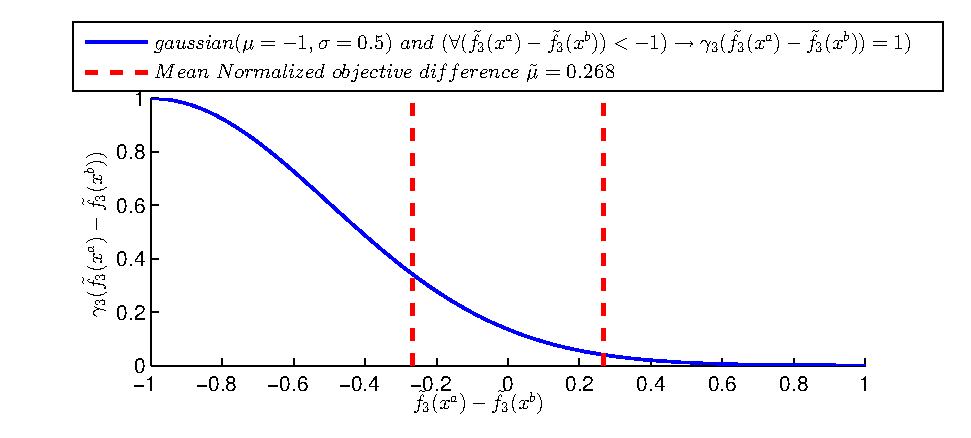
\includegraphics[width=3.3in,height=1.50in]{figures/relatedworks/Ngaussianfunctionwfg2_3.eps}

\caption{Left Gaussian Membership Function. This particular case shows the position of mean nomalized objective difference value ($\bar{\mu_3}$) for the third  objective of WFG2 problem obtained from the $250^{th}$ generation of a particular seed.}
\label{fig:leftgaussianupdated}
\end{figure}

It is seen from Eq.~(\ref{eq:gaussianeqn}) that the Gaussian function is defined by two parameters, $c$ and $\sigma$. 
While $c$ represents mean and it is set to $-1$, $\sigma$ defines the spread of the Gaussian function and  it is set to $0.5$ as a compromise. It has been indicated that setting $\sigma$ too large or too small leads to the inability to discriminate $v\in [-1, 0]$  
or $v \in [0, 1]$~\citep{he2014fuzzy}. Even setting $\sigma$ in this way may create uneven discrimination between the entire domain of $v\in [-1, 1]$. This can be attributed from Fig.~\ref{fig:leftgaussianupdated} that the discrimination ability of $\gamma_g(v)$ for $v\in [-1, 0]$ and for $v \in [0, 1]$ is not similar because the curve's nature in the said ranges are not identical.
Pareto dominance based EMO algorithms compare two solutions ${\bf x}^a = x^a_1, x^a_2, \ldots, x^a_n$  and ${\bf x}^b = x^b_1,x^b_2, \ldots, x^b_n$  based on their objective vectors ${\bf f}({\bf x}^a) = f_1({\bf x}^a), f_2({\bf x}^a), \ldots, f_m({\bf x}^a)$ and ${\bf f}({\bf x}^b) = f_1({\bf x}^b), f_2({\bf x}^b), \ldots, f_m({\bf x}^b)$, respectively. In line with this, fuzzy based  EMO algorithms utilize the difference of  objective vectors as the argument of the membership function i.e., $v = f_i({\bf x}^a) - f_i({\bf x}^b)$ or $v = f_i({\bf x}^b) - f_i({\bf x}^a)$.

An MaOP may or may not have an identical range of values for its each objective, 
$f_i$. To handle this issue, we may use a different membership function for each of 
different objectives i.e.,  a separate $\sigma$ for each objective. A similar concept is used in~\citep{farina2004fuzzy} where $\sigma$ is chosen manually.
 This will, however, require rich domain knowledge for each problem we like to solve.
Alternatively, we may normalize $v$ by the maximum difference among all pairs of solutions in that 
objective and can use the same membership function for all objectives. This alternative approach is used in some previous studies~(e.g.~\citep{he2014fuzzy}). The downside of normalization is the loss of information and influence of very large/small isolated value(s).

%Table~\ref{table:gaussianexample2} explains the aforementioned fact. In this particular scenario, there are two solutions $\textbf{x}^a$ and $\textbf{x}^b$ having objectives, $f_1$ and $f_2$. The objectives'
%differences with respect to these solutions i.e., $f_1({\bf x}^a) - f_1({\bf x}^b)$
%and $f_2({\bf x}^a) - f_2({\bf x}^b)$ are $-0.02$ and $0.08$, respectively.
%For a minimization problem, the negative and positive signs indicate that ${\bf x}^a$  and ${\bf x}^b$ are better with respect to its counterpart, respectively. Clearly, the improvement of ${\bf x}^a$ with respect to $f_1$  is less than that of ${\bf x}^b$ with 
%respect to $f_2$. Let the maximum objective difference of $f_1$ ($df_1^{max}$) is 0.3 and that of $f_2$ ($df_2^{max}$) is 1.5. The normalized objective differences for $\textbf{x}^a$ to $\textbf{x}^b$ in $f_1$ and $f_2$ are $-0.0667$ and $0.0533$, respectively. These differences indicate the relative improvement of $\textbf{x}^a$ over $\textbf{x}^b$ with respect to $f_1$ and $f_2$. 
%It is now evident that if the objective values are in different range we can have an improper impact on membership values through normalization.
%
%\begin{table}[!h]
%\centering
%\caption{Effect of normalization in the Gaussian member function}
%\label{table:gaussianexample2}
%\setlength{\tabcolsep}{2pt}
%\renewcommand{\arraystretch}{1.1}
%\begin{tabular}{lll}
%\thickhline
%\multicolumn{2}{l|}{Max. Abs. Obj. Difference of $f_1$ $(df_1^{max})$}              & 0.3            \\
%\multicolumn{2}{l|}{Max. Abs. Obj.  Difference of $f_2$ $(df_2^{max})$}              & 1.5            \\\thickhline
%\multicolumn{1}{l|}{Solution}               & $f_1(.)$   & $f_2(.)$   \\\thickhline
%\multicolumn{1}{l|}{$\textbf{x}^a$}                     & 0.2            & 0.2            \\
%\multicolumn{1}{l|}{$\textbf{x}^b$}                     & 0.22           & 0.12           \\\hline
%\multicolumn{1}{l|}{$ v_i = f_i(\textbf{x}^a)-f_i(\textbf{x}^b)$}         & -0.02          & 0.08           \\
%\multicolumn{1}{l|}{$\overline{v} = v/df_i^{max}$}   & -0.0667 & 0.0533  \\
%\multicolumn{1}{l|}{$\gamma_g(\overline{v})$}  & 0.1397   & 0.0867  \\\hline
%\multicolumn{1}{l|}{$ v = f_i(\textbf{x}^b)-f_i(\textbf{x}^a)$}         & 0.02           & -0.08          \\
%\multicolumn{1}{l|}{$\overline{v} = v/df_i^{max}$}   & 0.0667  & -0.0533 \\
%\multicolumn{1}{l|}{$\gamma_g(\overline{v})$} & 0.0819  & 0.1329   \\\thickhline
%%\multicolumn{2}{l|}{$dom(\textbf{x}^2,\textbf{x}^3)=\prod^{2}_{i=1}g_i(\overline{d}(f_i(\textbf{x}^2)-f_i(\textbf{x}^3)))$}                 & 0.0121  \\
%%\multicolumn{2}{l|}{$dom(\textbf{x}^3,\textbf{x}^2)=\prod^{2}_{i=1}g_i(\overline{d}(f_i(\textbf{x}^3)-f_i(\textbf{x}^2)))$}                 & 0.0109  \\
%%\multicolumn{2}{l|}{$\phi(\textbf{x}^2,\textbf{x}^3)=\frac{dom(\textbf{x}^2,\textbf{x}^3)}{dom(\textbf{x}^2,\textbf{x}^3)+dom(\textbf{x}^3,\textbf{x}^2)}$}                             & 0.5266   \\
%%\multicolumn{2}{l|}{$\phi(\textbf{x}^3,\textbf{x}^2)=\frac{dom(\textbf{x}^3,\textbf{x}^2)}{dom(\textbf{x}^2,\textbf{x}^3)+dom(\textbf{x}^3,\textbf{x}^2)}$}                             & 0.4733   \\\thickhline
%\end{tabular}
%\end{table}

%We have already raised two important issues of the membership function in the fuzzification step. They are uneven discrimination ability and normalization of the objective difference. 

In the inference step, to compute dominance of one solution with respect to other (e.g. $\textbf{x}^a$ over $\textbf{x}^b$), the fuzzy membership values of $m$-objective differences ($f_i({\bf x}^a)-f_i({\bf x}^b), i=1,2,\cdots,m$) are combined.                                                                                                                                                                 Irrespective of the type of membership function, any suitable fuzzy set theoretic operation can be used for 
combination~\citep{mendel1995fuzzy}. %Table~\ref{table:fuzzysetoperation} shows some typical inference operations. The fuzzy intersection set operation is generally used for a minimization problem. 
The most popular intersection set operation used in MaOPs is the product operation, also known as $t$-norm operation. 

\begin{comment}
%\vspace{-20pt}
\begin{table}[!h]
\centering
\caption{Some common fuzzy set operations to combine membership values in the inference step
of fuzzy logic}
\label{table:fuzzysetoperation}
\setlength{\tabcolsep}{2pt}
\renewcommand{\arraystretch}{1.1}
\begin{tabular}{c|c}
\thickhline
OR(Union) & And(Intersection) \\\thickhline
$Max(\{\gamma_1(v_1),\gamma_2(v_2)\})$          & $Min(\{\gamma_1(v_1),\gamma_2(v_2)\})$     \\
$\gamma_1(v_1)+\gamma_2(v_2)-\gamma_1(v_1)\times\gamma_2(v_2)$          & $\gamma_1(v_1)\times\gamma_2(v_2)$\\
$Min(\{1,\gamma_1(v_1)+\gamma_2(v_2)\})$          & $Max(\{0,\gamma_1(v_1)+\gamma_2(v_2)-1\})$     \\\thickhline
\end{tabular}
\end{table}
\end{comment}

%\vspace{-20pt}
The following equations show the fuzzy inference and relative dominance computation procedure of two $m$-objective solutions, $\textbf{x}^a$ and $\textbf{x}^b$.
\begin{align}
	 dom({\bf x}^a, {\bf x}^b) = \prod^{m}_{i=1} \gamma_i(f_i({\bf x}^a)-f_i({\bf x}^b))\label{eq:domi1}\\
	 dom({\bf x}^b, {\bf x}^a) = \prod^{m}_{i=1} \gamma_i(f_i({\bf x}^b)-f_i({\bf x}^a))\label{eq:domi2}
\end{align}

\begin{eqnarray}
\phi({\bf x}^a, {\bf x}^b)=\frac{dom({\bf x}^a, {\bf x}^b)}{dom({\bf x}^a, {\bf x}^b) + dom({\bf x}^b, {\bf x}^a)}\label{eq:re-domi1} \\
\phi({\bf x}^b, {\bf x}^a)=\frac{dom({\bf x}^b, {\bf x}^a)}{dom({\bf x}^a, {\bf x}^b) + dom({\bf x}^b, {\bf x}^a)}\label{eq:re-domi2}
\end{eqnarray}

\noindent where  $dom({\bf x}^i, {\bf x}^j)$ is  a scalar value and represents  how much $\textbf{x}^a$ dominates 
$\textbf{x}^b$. The term  $\phi({\bf x}^a, {\bf x}^b)$ indicates the relative dominance of ${\bf x}^a$ to ${\bf x}^b$. We consider ${\bf x}^a$ dominates ${\bf x}^b$ iff $dom({\bf x}^a, {\bf x}^b) > dom({\bf x}^b, {\bf x}^a)$ and non-dominated iff $dom({\bf x}^a, {\bf x}^b) = dom({\bf x}^b, {\bf x}^a)$.
It is evident from the above relations that if one solution is Pareto dominated then it  will also be fuzzy dominated and if two solutions are fuzzy non-dominated they are Pareto non-dominated. 
However, it is very unlikely that two different solutions will have a same fuzzy dominance value (fuzzy non-dominated) even though they are Pareto non-dominated. Because of the different objective differences, fuzzy dominance is able to discriminate two solutions even when they are Pareto non-dominated. Therefore Pareto dominance can be considered as a special case of fuzzy dominance.
  
In defuzzification step, the dominance impact of one solution with respect to other solutions can be combined, ranked 
or used instead of Pareto 
dominance~\citep{he2014fuzzy,he2012new,koppen2005fuzzy,farina2004fuzzy,fuzzynasir}. An important observation is that irrespective of a membership function and a set theoretic operation, we end up with only a scalar fuzzy value which does not tell anything about diversity. If the solutions are selected solely based on the fuzzy dominance values, the chosen solutions will be less diverse and will not able to cover the entire Pareto front of a given problem. This can be seen from the experimental evidences provided in a recent study~\citep{sdealgorithm}. Some existing approaches (e.g.~\citep{he2014fuzzy}, \citep{fuzzynasir}) use a threshold parameter to divide solutions into different fronts but still fails to provide enough diversity in high-dimensional and non-regular Pareto~\citep{rectangleproblem}.

%In summary, with respect to existing fuzzy works, three issues need to be addressed while using fuzzy dominance in an EMO algorithm. These include uneven discrimination ability of the membership function, normalization of the objective difference and loss of diversity during environmental selection. 


\subsection{Related Work}
There are a very few fuzzy based EMO algorithms in the literature. 
%In~\citep{he2014fuzzy,he2012new}, the authors utilized fuzzy dominance concept to continuously differentiate individuals of a population into different degrees of optimality beyond the classification of the original Pareto dominance. They used  the same left Gaussian function as a membership function for all objectives of a given MaOP. To maintain diversity, the authors used a user-defined parameter.  The fuzzy concept was incorporated into the designs of NSGA-II and SPEA2 as a case study.


%\citep{he2014fuzzy,he2012new,koppen2005fuzzy,farina2004fuzzy,fuzzynasir}

%Farina and Amato~\citep{farina2004fuzzy} proposed different fuzzy-based definitions of optimality and used preference information to incorporate human decision making. A parameter used and when its value is zero, the introduced definitions coincide with classical Pareto-optimality. If the value is increased (maximum one), then different subset of Pareto optimal solutions can be obtained corresponding to higher degrees of optimality.


In~\citep{farina2004fuzzy}, Farina and Amato proposed definitions of fuzzy-based optimality for multi-objective optimization. The main idea behind the given definitions is to introduce different degree of optimality. 
For each objective, the authors used a combination of three Gaussian functions as a non-adaptive membership function. The purpose of such a combined mechanism is to distinguish amongst better, equal and worse objective differences between two solutions. The proposed definitions have been applied on two simple multi-criteria decision making problems and two MOPs. 


%In~\citep{fuzzynasir}, Nasir et al. introduced a decomposition based fuzzy dominance algorithm (MOEA/DFD) where a fuzzy Pareto dominance concept is used to compare two solutions and used the scalar decomposition method only when one of the solutions fails to dominate the other in terms of a fuzzy dominance level.




%In~\citep{koppen2005fuzzy} Koppen and Garcia incorporated generic ranking scheme where the vector fitness values of a population can be replaced by the computed ranking values (representing the ``dominating strength`` of an individual against all other individuals in the population) and used to perform standard single-objective genetic operators. Based on that Fuzzy-Dominance Driven GA (FDD-GA), was proposed.

The work described in~\citep{koppen2005fuzzy} studied the fuzzyfication of Pareto dominance relation and its application to the design of an EMO algorithm. In fuzzyfication, the authors used a non-symmetric membership function. Solutions those have high performance in one objective but poor in others will be preferred in the given fuzzy dominance definition. As no additional diversity measure was used in~\citep{koppen2005fuzzy}, the evolving population will lose diversity.
To verify the usefulness of proposed EMO algorithm, an analytic study of the Pareto-Box problem was provided.

Nasir {\it et al.}~\citep{fuzzynasir} introduced a decomposition based fuzzy dominance algorithm (MOEA/DFD). For all objectives, the algorithm uses a general membership function of $Ae^{-x}$ with uneven discrimination power. As the same membership function is used for all objectives, scaling issues are not addressed here. In comparing solutions, MOEA/DFD employed fuzzy dominance when a solution's dominance level   is found greater than a particular threshold value. Otherwise, it used decomposition based weighted approach, which is able to handle diversity.
The performance of MOEA/DFD was evaluated on twelve benchmark problems having two-objective to five-objective.


In~\citep{he2014fuzzy,he2012new}, the authors utilized fuzzy dominance concept to continuously differentiate individuals of a population into different degrees of optimality. They used  the same left Gaussian function as a membership function for all objectives of a given MaOP. 
To handle the scaling issue, the objective differences are normalized by corresponding maximum objective difference value. The fuzzy concept was incorporated into NSGA-II and SPEA2 as a case study and termed them  FD-NSGA-II and FD-SPEA2. In FD-NSGAII, a threshold value is used to divide solutions into different fronts based on the fuzzy dominance value. However, the solutions in the last front are chosen based on crowding distance. As fuzzy dominance is capable of discriminating solutions, crowding distance will rarely be used. 
Moreover, crowding distance has already found to be ineffective on MaOPs~\citep{purshouse2007evolutionary,deb2014evolutionary,thetadominance7080938}.
In FD-SPEA2, the best $N$ solutions for next generation are taken based on fuzzy dominance values.
The performance of the proposed algorithm was evaluated on seven DTLZ problems and two WFG problems having 5-, 10- and 20-objective.


%The proposed framework described in the following section uses a preferred reference point based clustering along with adaptive Sigmoid membership function to deal with the issues commonly faced by other fuzzy based approaches. While the preferred reference point based clustering is used to deal with diversity promotion (section~\ref{subsec:clustering}), the adaptive membership function~(\ref{subsec:membershipFunction}) is employed to handle the objective scaling issue.

%\subsection{Related Reference Points and Clustering Approaches}
%
%
% The reference points and evolved solutions are considered in $F$-DEA as the clusters' centers and members, respectively. Existing works~(e.g.~\citep{deb2014evolutionary,thetadominance7080938,deb2006reference,piceag,referencevectorguided} ) generally utilize reference points in some way for assigning fitness to the solutions.
%
%Some previous non-fuzzy studies~\citep{thetadominance7080938,deb2014evolutionary,coellotwoapproach} also employ clustering in EMO algorithms.  
%
%The clustering procedure of $F$-DEA differs from NSGAIII~\citep{deb2014evolutionary} with two notable exceptions. Firstly, $F$-DEA employs preferred reference points based clustering to provide better cluster uniformity, remove dependency on population size and handle irregular shaped Pareto fronts.
% Secondly, $F$-DEA employs cosine similarity instead of Euclidean distance to find the solutions' association
%	with the generated reference points. It is suitable  because angle between a reference point and a candidate solution remains constant irrespective of exact distance from the ideal point, which handles the scaling issue of the generated reference points. The  $\theta$-dominance algorithm~\citep{thetadominance7080938} also uses reference points based clustering similar to NSGAIII with an exception in normalization procedure. In~\citep{coellotwoapproach},  clustering based elitist genetic algorithm (CEGA) uses  a bottom up hierarchical approach  in the decision variable space not in the objective space. %The basic notion of CEGA is that convergence with a poorly spread set of Pareto-optimal solutions is preferred than a well-spread set of solutions which are far from the Pareto-optimal surface. The procedure and notion of this clustering is different from the one we employ in $F$-DEA. The investigation of how different clustering approaches work in the context of $F$-DEA is outside the scope of this paper and would be the topic of a separate paper.
%
%The proposed framework described in the following section uses a preferred reference point based clustering approach along with adaptive Sigmoid membership function to deal with the issues commonly faced by other fuzzy based approaches. 


\section{Proposed Algorithm}
\label{sec:ourapproach}

%\textbf{Algorithm's key feature, novelty}

In order to avoid the detrimental effect of uneven discrimination and objective normalization, $F$-DEA employs a separate membership function for each objective and determines its parameters adaptively. 
%We here argue that it is better to use a separate membership function with adaptive parameters while solving MOPs using fuzzy based EMO algorithms. 
It also employs preferred reference points based clustering for ensuring diversity in its environmental selection.  
These features make the proposed algorithm different from others.

%\textbf{From the previous section we can realize that the fuzzy concept is particularly suitable for many objective problem as it can effectively offer comparability among non-dominated solutions for large number of objectives. The proposed $F$-DEA utilizes this notion and handles the issues faced by existing approaches. 

%Adopting only the fuzzy dominance relation is not sufficient for an evolutionary algorithm to solve MaOPs with good convergence and diversity. It is because no technique is embedded in such a dominance relation for ensuring diversity. This is also true for the Pareto dominance relation. The proposed $F$-DEA thus utilizes the concept of reference points in conjunction with fuzzy dominance for balancing between convergence and diversity while solving MaOPs. Unlike existing reference points based algorithms (e.g.~\citep{wang2013preference,deb2006reference,jin2002incorporation}), $F$-DEA employs reference points for constructing clusters using the solutions of an evolving population.

The algorithm  starts with a randomly generated parent population $P_t$ of $N$ solutions and a set of generated/supplied reference points $R^g/R^s$. It then creates an offspring population $Q_t$ of size $N$ by applying crossover and mutation. 
%All the solutions in the combined population $C_t$ (=$P_t \bigcup Q_t$) and the reference points  may reside at different regions of the $m$-dimensional objective space. 
Based on the positional information in the objective space, $F$-DEA finds $p$ preferred points ($p\le N$) and constructs clusters using the solutions as members  and the preferred points as centers.
It then adaptively constructs $m$ fuzzy membership functions i.e., one function for each objective 
and utilizes them to compute dominance degrees of the solutions. Finally, $F$-DEA assigns fitness to the solutions and selects the best ones from different clusters in a round-robin fashion to from a new population $P_{t+1}$ for the next generation.  
We summarize the steps of our method in Algorithm 1, which are explained further as follows.



%%%%%%%%%%%%%%%%Complete Algorithm%%%%%%%%%%%%%%%%%%%%%%%%

\begin{algorithm}[!h]
	
	\textbf{Input:} $R^g/R^s$ (generated reference points or supplied points), $P_t$ (parent population of $t$-th generation), $N$ (population size)\\
	\textbf{Output:} $P_{t+1}$
	
	\begin{algorithmic}[1]
		\STATE $Q_t \gets $ Recombination and Mutation on $P_t$
		\STATE $C_t \gets P_t \cup Q_t$				
		\STATE Select $p\le N$ preferred reference points:\\ $R^p \gets PreferredReferencePoint(C_t, R^g/R^s, p)$	
		\STATE Construct clusters using $R^p$:\\ $R^p(\{{\bf r}^j,X({\bf r}^j)|1\le j\le p\})$ \% ${\bf r}^j$: $j$-th reference point in $R^p$, $X({\bf r}^j)$: associated solution with ${\bf r}^j$
		\STATE Construct $m$ membership functions:\\$(\gamma_1,\gamma_2\cdots\gamma_m) \gets AdaptiveMembershipFunction(C_t)$		
		\STATE Assign fitness to solutions within individual cluster:\\ $FitnessAssignment(R^p,C_t,\gamma)$
		\STATE Sample solution from each cluster:\\ $P_{t+1}\gets SamplingSelection(R^p,N)$
		
	\end{algorithmic} 
	
	\caption{Generation $t$ of $F$-DEA}
	
	\label{alg:completeAlgorithm}
\end{algorithm}

%%%%%%%%%%%%%%%%%Preferred REference Point%%%%%%%%%%%%%%%%%

\begin{algorithm}[!h]
	
	\textbf{Input:} $R^g/R^s$, $C_t$ (combined population), $p$ (maximum size of preferred reference points)\\
	\textbf{Output:}  $R^p(\{{\bf r}^j,X({\bf r}^j)|1\le j\le p\})$ $($set of preferred reference points ${\bf r}^j$s with associated cluster of solutions $X({{\bf r}^j})s)$
	
	\begin{algorithmic}[1]
		
		\FOR{each solution ${\bf x} \in C_t$}
			\STATE Normalize $f({\bf x})$: $\tilde{f}({\bf x}) = \tilde{f}_1({\bf x}),\tilde{f}_2({\bf x}),\ldots\tilde{f}_m({\bf x})$
		\ENDFOR
		
		%STATE Normalize the objective values $({\bf f}^{nor}({\bf x}) = f_1^{nor}({\bf x}),  f_2^{nor}({\bf x}), \ldots f_m^{nor}({\bf x}))$ of each  solution ${\bf x} \in C_t$
		
		\STATE $R^{a} = \{\emptyset\}$ 
		%\STATE $E = \emptyset$
		
		\FOR{each solution ${\bf x} \in C_t$}
		\STATE $\mathbf{r}= {\mathbf{r^g}:\argmax_{\mathbf{r^g}\in R^g/R^s}({S(\mathbf{r^g},\tilde{\bf f}({\bf x})))}}$
		\IF{$\mathbf{r} \notin R^a$}
		\STATE $X(\mathbf{r}) =\{\bf x\}$
		\STATE $R^a = R^a \bigcup \{\mathbf{r}\}$
		\ELSE
		\STATE $X(\mathbf{r}) = X(\mathbf{r}) \bigcup \{\mathbf{x}\}$ 
		\ENDIF
		%\STATE $E= E \bigcup \{X^r\}$
		\ENDFOR
		
		
		\IF{$\left|R^{a}\right| > p$}
		\STATE Sort $R^a$: $MinMax(R^a)$
		\STATE $R^p$ = First $p$ points of $R^a$
		\STATE $R^r = (R^a-R^p)$
		\FOR{each ${\mathbf{r}^r \in R^r}$}
		\FOR{each solution ${\bf x} \in X({{\bf r}^r})$}
		\STATE $\mathbf{r}= {{{\bf r}^p}:\argmax_{{{\bf r}^p}\in R^p}({S({{\bf r}^p},\tilde{\bf f}({\bf x})))}}$
		\STATE $X({\bf r})$=$X({\bf r}) \bigcup \{\bf x\}$ 
		\ENDFOR
		
		\ENDFOR	
		
		\ELSE	
		\STATE $R^p$ = $R^a$	 	 	
		\ENDIF
		
	\end{algorithmic}
	\caption{$PreferredReferencePoint(C_t, R^g/R^s, p)$ }
	
	\label{alg:prefferedReferencePoint}
\end{algorithm}



%%%%%%%%%%%MinMax%%%%%%%%%%%%%%%%%%%%

\begin{algorithm}[!h]
	
	\textbf{Input:} $R$ (reference points)\\
	\textbf{Output:} $R^{st}$ (reference points sorted according to $MinMax$ distance)
	
	\begin{algorithmic}[1]
		
		\STATE $R^{st} = \emptyset$
		\STATE $R^m$ = A set of $m$ extreme points (one for each objective) chosen from $R$ 
		\STATE $R^{st} = R^{st} \bigcup R^m$
		\STATE ${R}^\prime = R-R^{st}$
		\FOR{\textbf{each} $\mathbf{r}$ in ${R}^\prime$}	
		\STATE Distance measure: $dist(\mathbf{r})=\displaystyle\min\limits_{\forall \mathbf{r}^{st} \in R^{st}}{d(\mathbf{r}, \mathbf{r}^{st})}$
		\ENDFOR
		
		\WHILE {${R}^\prime \neq \emptyset$}
		\STATE $\mathbf{r}^b =\mathbf{r}:\argmax_{\mathbf{r}\in R^\prime} dist(\mathbf{r})$
		\STATE $R^s=R^s \bigcup \{\mathbf{r}^b\}$
		\STATE ${R}^\prime = {R}^\prime-\{\mathbf{r}^b\}$	
		
		\FOR{\textbf{each} $\mathbf{r}$ in ${R}^\prime$}							
		\STATE Update: $dist(\mathbf{r})=\displaystyle\min{(dist(\mathbf{r}),d(\mathbf{r},\mathbf{r}^b))}$
		\ENDFOR
		
		\ENDWHILE	
		
	\end{algorithmic}
	\caption{$MinMax(R)$}
	
	\label{alg:MinMaxAlgo}
\end{algorithm}


%%%%%%%%%%%%%%%%Adaptive Membership Function%%%%%%%%%%%%%%%%%%%

%\begin{algorithm}[!h]
%	
%	\textbf{Input:} $C_t$\\
%	\textbf{Output:} $\gamma = \gamma_1, \gamma_2, \ldots \gamma_m$ (membership functions for $m$ objectives)
%	
%	\begin{algorithmic}[1]
%		\FOR{$i = 1 \ \text{to} \ m$}
%			\STATE Compute mean $\mu_i$ and variance $\sigma_i^2$ from the pair-wise objective value differences, $|f_i({\bf x}^a)-f_i({\bf x}^b)|$, of all solutions in $C_t$% using Eqs.~(\ref{eq:meanvalue}) and~(\ref{eq:varianevalue}).
%			\STATE Compute growth rate $\alpha_i$ from $\mu_i$ and $\sigma_i^2$ using Eq.~(\ref{eq:alpha})% 	\STATE Compute growth rate $\alpha_i$, from $\mu_i$ and $\sigma_i$ using  equation \ref{eq:alphaCalculation}
%			\STATE Construct the membership function $\gamma_i$ with $\mu_i$ and $\alpha_i$ as its parameters using Eq.~(\ref{eq:SigmoidFunction})
%		\ENDFOR
%		
%	\end{algorithmic}
%	\caption{$AdaptiveMembershipFunction(C_t)$}
%	
%	\label{alg:adaptivemembershipfunction}
%\end{algorithm}


%%%%%%%%%%%%%%%%%%%%Fuzzy domination degree%%%%%%%%%%%%%%%%%%%%


%\begin{algorithm}[!h]
%	\textbf{Input:} $\mathbf{x}^a,\ \mathbf{x}^b,\ \gamma$\\
%	\textbf{Output:} $[\phi(\mathbf{x}^a, \mathbf{x}^b),\phi(\mathbf{x}^b, \mathbf{x}^a)]$
%	(dominance degree of $\mathbf{x}^a$ over $\mathbf{x}^b$ and $\mathbf{x}^b$ over $\mathbf{x}^a$)
%	
%	\begin{algorithmic}[1]
%		\STATE Compute $dom(\mathbf{x}^a, \mathbf{x}^b), dom(\mathbf{x}^b, \mathbf{x}^a)$ using Eqn.\ref{eq:domi1}, \ref{eq:domi2}
%		\STATE Compute $\phi(\mathbf{x}^a, \mathbf{x}^b),\phi(\mathbf{x}^b, \mathbf{x}^a)$ using Eqn.\ref{eq:re-domi1}, \ref{eq:re-domi2}
%%		\STATE $dom(\mathbf{x}^a,\mathbf{x}^b)=dom(\mathbf{x}^b,\mathbf{x}^a)=1$
%%		\FOR{$i=1$ to $m$}
%%			\STATE $dom(\mathbf{x}^a,\mathbf{x}^b)=dom(\mathbf{x}^a,\mathbf{x}^b)\times\gamma_{i}(f_i({\bf x}^a)-f_i({\bf x}^b))$
%%			
%%			\STATE $dom(\mathbf{x}^b,\mathbf{x}^a)=dom(\mathbf{x}^b,\mathbf{x}^a)\times\gamma_{i}(f_i({\bf x}^b)-f_i({\bf x}^a))$
%%		\ENDFOR
%%		\STATE $\phi(\mathbf{x}^a,\mathbf{x}^b)=\frac{dom(\mathbf{x}^a,\mathbf{x}^b)}{dom(\mathbf{x}^a,\mathbf{x}^b)+dom(\mathbf{x}^b,\mathbf{x}^a)}$
%%		\STATE $\phi(\mathbf{x}^b,\mathbf{x}^a)=\frac{dom(\mathbf{x}^b,\mathbf{x}^a)}{dom(\mathbf{x}^a,\mathbf{x}^b)+dom(\mathbf{x}^b,\mathbf{x}^a)}$
%		
%		% \STATE \textbf{return} $[\phi(\mathbf{x}_a,\mathbf{x}_b),\phi(\mathbf{x}_b,\mathbf{x}_a)]$
		
%	\end{algorithmic}
%	\caption{$FuzzyDominance({\bf x}^a,{\bf x}^b,\gamma)$}
%	
%	\label{alg:FuzzyDominaceAlgo}
%\end{algorithm}



%%%%%%%%%%%%%Fitness Assignment%%%%%%%%%%%%%%%%

%\begin{algorithm}[!h]
%	
%	\textbf{Input:} $R^p,\ C_t,\ \gamma$\\
%	\textbf{Output:} Fitness values of all solutions in $C_t$
%	
%	\begin{algorithmic}[1]
%		\FOR{\textbf{each} $\bf r$ in $R^p$}
%		
%			\FOR{$a=1$ to $\left|{X(\mathbf{r})}\right|$}					
%
%				\STATE $\mathbf{x}^a = a^{th}$ solution of ${X(\mathbf{r})}$
%%				\STATE $fit(\mathbf{x}^a)=0$
%				\STATE $fit(\textbf{x}^a)=  \sum_{b=1, b\neq a}^{b=\left|X(\mathbf{r})\right|} \phi(\textbf{x}^b,\textbf{x}^a)$\\ $[\phi(\mathbf{x}^a,\mathbf{x}^b),\phi(\mathbf{x}^b,\mathbf{x}^a)] = FD(\mathbf{x}^a,\mathbf{x}^b,\gamma)]$
%				
%%				\FOR{$b=a+1$ to $\left|{X(\mathbf{r})}\right|$}
%%	
%%					\STATE $\mathbf{x}^b = b^{th}$ solution of ${X(\mathbf{r})}$
%%				
%%					\STATE $[\phi(\mathbf{x}^a,\mathbf{x}^b),\phi(\mathbf{x}^b,\mathbf{x}^a)] = FD(\mathbf{x}^a,\mathbf{x}^b,\gamma)$			
%%					\STATE $fit(\mathbf{x}^a)=fit(\mathbf{x}^a)+\phi(\mathbf{x}^b,\mathbf{x}^a)$ 					
%%					\STATE $fit(\mathbf{x}^b)=fit(\mathbf{x}^b)+\phi(\mathbf{x}^a,\mathbf{x}^b)$ 	
%%	
%%				\ENDFOR
%	
%			\ENDFOR
%		\ENDFOR
%		
%	\end{algorithmic}
%	\caption{$FitnessAssignment(R^p,C_t,\gamma)$}
%	
%	\label{alg:FitAssignAlgo}
%\end{algorithm}


%%%%%%%%%%%%%subsection{Sampling and Selection algorithm}%%%%%%%%%%%%


%\begin{algorithm}[!h]
%	\textbf{Input:} $R^p, N$\\
%	\textbf{Output:} $P_{t+1}$
%	\begin{algorithmic}[1]
%		\STATE Sort $R^p$: $MinMax (R^p)$
%		\STATE $j = 0$
%		\STATE $P_{t+1} = \emptyset$
%		\WHILE{$\left|P_{t+1}\right|<N$}
%		\STATE $j^{th}$ Reference Point: $\mathbf{r}^j = R^p(j)$
%		\IF{$\left|{X(\mathbf{r}^j)}\right|>0$}
%		\STATE $P_{t+1} = P_{t+1}\cup \{\mathbf{x}: fit(\mathbf{x})= \min_{\mathbf{x} \in {X(\mathbf{r}^j)}}{fit(\mathbf{x})} \}$
%		\STATE ${X(\mathbf{r}^j)}={X(\mathbf{r}^j)}-\{\mathbf{x}\}$
%		\ENDIF
%		\STATE $j = (j+1)\mod N$
%		\ENDWHILE
%		
%	\end{algorithmic}
%	\caption{$SamplingSelection(R^p,N)$}
%	
%	\label{alg:EnvSelectionAlgo}
%\end{algorithm}



\subsection{Reference Point Generation}
\label{subsec: globalReferencePoint}
A number of existing studies~\citep{deb2014evolutionary,thetadominance7080938,
deb2006reference,piceag,referencevectorguided,epcs} employ reference points for assigning fitness values. However, $F$-DEA uses 
such points for clustering the solutions with a hope of maintaining both convergence and diversity. There are two important 
considerations for generating the reference points. 
Firstly, the reference points are to be generated in such a way so that they are uniformly distributed over the $m$-dimensional objective space. 
%However, such a generation procedure may be problematic for an MOP with a degenerate Pareto front. The proposed $F$-DEA tries to alleviate this problem to some extent by using the information of the reference points' association with the existing solutions. 
Secondly, the generation procedure has to be scaleable and computationally efficient. Keeping these considerations in mind, $F$-DEA uses the Das and Dennis's procedure~\citep{das1998normal} like others~\citep{deb2014evolutionary,zhang2007moea,thetadominance7080938} for generating the reference points, which are  distributed uniformly along the $m$-dimensional hyper-plane. %, $\overline{W}^T\times\overline{B}=1$. Here, $\overline{W}$ is an $m$-dimensional unit hyper-plane and $\overline{B}$ is any point on the hyper-plane. 
The procedure generates a set of reference points, $R^g$, spanning the whole plane, each at $\delta = \frac{1}{\lambda}$ distance apart from the others. Analytically, $\left|R^g\right| = \binom{m+\lambda-1}{\lambda}$ reference points are generated where $\lambda$ denotes the number of divisions in each objective-coordinate.

The main problem of this generation procedure or others~\citep{zhang2007moea} is the exponential increase of reference points with the increase of objectives. A simple technique to handle this issue is to increase the population size with respect to $\left|R^g\right|$. This in turn  will increase evolution time. As an alternative, some studies (e.g.~\citep{thetadominance7080938,deb2014evolutionary}) generate a smaller number of reference points and impose this number as a constraint on the population size. $F$-DEA, on the other hand, first generates a large number reference points and then selects a set of  preferred points based on the population size. This alleviates the problem of imposing constraint on the population size.

%\subsection{Offspring Creation}
%\label{subsec:offSpringpop}

%{\bf At generation $t$, $F$-DEA creates an offspring population $Q_t$ of size $N$ using simulated binary crossover and polynomial  mutation. In doing so, it first creates a mating pool by applying \sout{binary} tournament selection on the parent population $P_t$. The crossover operator then produces an offspring from a pair of solutions of the mating pool. Finally, $F$-DEA refines offspring by applying mutation on  it.}


\subsection{Preferred Reference Point}
\label{subsec:prefereableReferencePoint}

All the generated reference points may not be equally important with respect to the existing solutions of an evolving population. 
The proposed $F$-DEA thus selects a set of preferred reference points, $R^p$. It first finds the 
active reference points from $R^g/R^s$ and then applies the {\it MinMax} procedure on them  
to choose $p$ diverse points. A reference point is called an active reference point if it maintains 
some associations with one (or more) solution(s). The upper bound of $p$ i.e., $|R^p|$
is $N$, the population size. The solutions of a population may reside in some (not all) regions of the 
$m$-dimensional objective 
space. In that case, $p$ will be less than $N$. Our algorithm
constructs $p$ clusters using the preferred points as their centers and the solutions of $C_t$ as their members. 
The procedure for selecting the preferred reference points and clusters is given in Algorithm~\ref{alg:prefferedReferencePoint}.
%{\Large We associate one solution in one cluster}

\subsubsection{Active Reference Point}
\label{subsubsec: activeReferencePoint}


As the values of the generated reference points lie in the range between 0 and 1, we adaptively 
normalize the objective values of the solutions to measure how close a solution is with respect to a particular reference point.
Following the adaptive normalization procedure of~\citep{deb2014evolutionary}, the $i$-th objective value, $f_i({\bf x}^a)$, of any solution ${\bf x}^a$ can be normalized as

\begin{equation} \label{eq:normalizedEquation}
	\tilde{f}_i({\bf x}^a) = \frac{f_i({\bf x}^a) - f_i^{min}({\bf x}^u)}{{\bf z}^i-f_i^{min}({\bf x}^u)} \ \ \ \forall i \in {1,2,\cdots, m}
\end{equation}

\noindent where $\tilde{f}_i({\bf x}^a)$ is the $i$-th normalized objective value of the solution ${\bf x}^a$. The symbol
$f_i^{min}({\bf x}^u)$ refers to the minimum value of the $i$-th objective with respect to all solutions in $C_t$ and 
the solution ${\bf x}^u$ has the minimum $i$-th objective value. The symbol ${\bf z}_i$ refers to the intercept computed 
from the $i$-th objective axis and a $m$-dimensional linear hyper-plane.
The  hyper-plane is constituted from $m$ solutions, where a solution ${\bf x}^h\in C_t$ makes the following achievement scalarizing function (ASF) minimum for an objective direction ${\bf w}_i$.

\begin{equation} \label{eq:achievementfunction}
	ASF({\bf x}^h, {\bf w}_i) = \max_{i=1}^{m} \frac{f({\bf x}^h)-f^{min}({\bf x}^u)}{{\bf w}_i} \ \ \ {\bf x}^h\in C_t
\end{equation}

\noindent Normalization using intercepts helps solutions to expand it's objective space.

The closeness of solutions indicates their associations with the reference points. We  utilize cosine similarity measure for this purpose. The cosine similarity measure, $S(\mathbf{r^j},\tilde{\bf f}({\bf x}^a))$, between the normalized fitness vector $\tilde{\bf f}({\bf x}^a) = \tilde{f}_1({\bf x}^a), \tilde{f}_2({\bf x}^a), \ldots \tilde{f}_m({\bf x}^a)$ of any solution ${\bf x}^a$ and the $m$-dimensional $j$-th reference point ${\bf r}^j$  can be computed as

\begin{equation} \label{eq:cosineSim}
	S(\mathbf{r^j},\tilde{\bf f}({\bf x}^a))=\frac{\tilde{\bf f}({\bf x}^a) . {\bf r}^j}{|\tilde{\bf f}({\bf x}^a)||{\bf r}^j|} \ \ \  \forall j \in {1, 2, \cdots, \left|R^g\right|}
\end{equation}

\noindent %Note that both $\tilde{\bf f}({\bf x}^a)$  and ${\bf r}^j$  have $m$ components.
As we generate a set of reference points, $R^g$, there will be $\left|R^g\right|$ similarity measures for 
${\bf x}^a$. The largest similarity measure obtained for any of the  reference points is considered as the active reference point that maintains the highest association with ${\bf x}^a$. %Computing Active Reference Points can be also considered as the clustering of solutions based on the Reference Points so the Active Reference Points can be called as the Cluster Points. 
While associating the solutions with the reference points, it is possible that some points may associate more than one solutions, some may associate one solution or some may associate no solution at all. %We present the procedure for computing active reference points  in Algorithm~\ref{alg:activeRefCalculation}.


\subsubsection{MinMax Measure}
\label{subsubsec:minMax}

The objective space size increases exponentially with an increasing number of objectives. It would be beneficial if we can cover 
the whole objective space by a reasonable number of active reference points in the least crowded manner. We devise a  procedure based on the \textit{MinMax} measure to select $p$ diverse active reference points, which $F$-DEA employs as the clusters' centers,  from the crowded ones~(Algorithm~\ref{alg:MinMaxAlgo}). 

The  procedure first selects  $m$ number of  most extreme active reference points i.e., one for each objective and then incrementally selects the other points. 
To select the other points,  it calculates the minimum Euclidean distance between the already selected points and the remaining  ones. The point with the maximum distance is selected as the next point and the minimum distance of the remaining points are updated based on the selected point. This procedure continues until all the points are selected.
In this way, we finally obtain a sorted list of active reference points
that are far apart from each other i.e., diverse. 
This procedure will be effective for disconnected, degenerated and other irregular shaped geometry because we are using the reference points only where solutions exist. Thus we are effectively maintaining cluster uniformity using the same number of reference points as other approaches but we are using them where it is needed.
%We could use other distance measure such as crowding distance. However, the crowding distances of several active reference points might be same  due to the way the Das and Dennis procedure~\citep{das1998normal} generates the reference points. It is not possible to select the diverse points based on crowding distance in such a scenario. Our {\it MinMax} measure avoids this sort of problem for which we use it  for selecting the diverse active reference points. 
It may possible to devise other techniques as well, which can be a future research topic. %{\bf Each selected point acts as the cluster center and its associated solutions as the cluster's members.} 
Fig.~\ref{fig:prefferedrefpointswfg2} demonstrates the process of selecting
the preferred reference points from a set of generated reference points.

 

%\input{clustermechanism}


%In this manner we obtain a sorted order of points $r_1, r_2,\cdots, r_{i-1}, r_i, r_{i+1},\cdots,r_{n}$ such that $\min_{l=1}^{i-1} d(r_i,r_l)>\forall_{j=i+1}^{n}(\min_{l=1}^{l=i-1}d(r_j,r_l))$

%Which means a point's minimum euclidean distance from the previous selected points is greater than the rest of the points. The algorithm for sorting points based on \textit{MinMax} distance is described in algorithm \ref{alg:incDistanceAlgo} 

\begin{figure*}[htbp] 
\centering    		
	\subfigure[$|R^g|=20$, Original Solutions $|C_t|=12$]
	{
		\label{fig:2trueandnormalizedsolutions}
		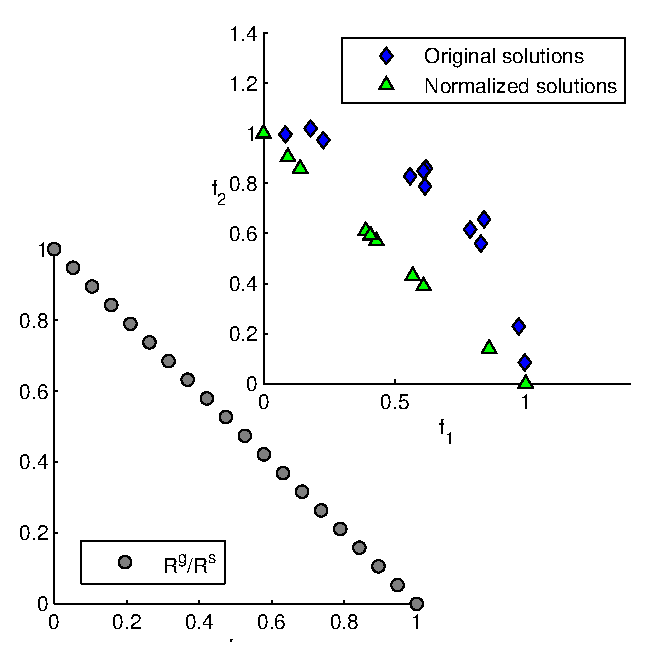
\includegraphics[width=1.50in]{figures/proposedalgorithm/sAlg1.eps}
	}
	~
	\subfigure[Active reference points $|R^a|=9$ (marked with vector line)]
	{
		\label{fig:2globalreferencepointstonormalize}
		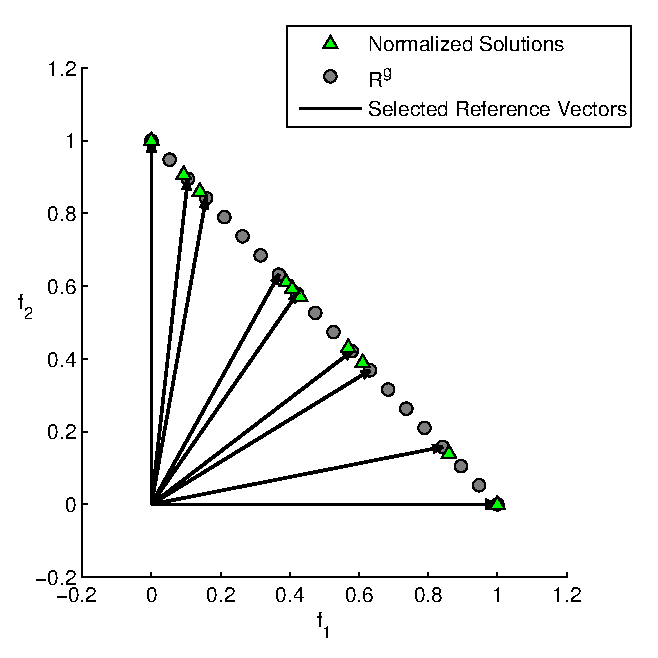
\includegraphics[width=1.50in]{figures/proposedalgorithm/sAlg2.eps}
	}	
	~	
	\subfigure[Selection of  a number of preferred reference points $(p = 6)$]
	{
		\label{fig:2minmaxreduction}
		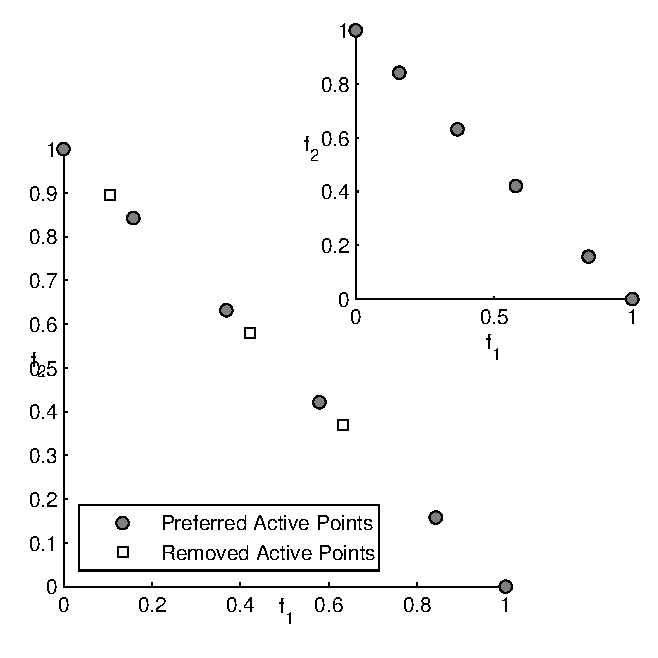
\includegraphics[width=1.50in]{figures/proposedalgorithm/sAlg3.eps}
	}	
\caption{Process of selecting
the preferred reference points from a set of generated reference points}
\label{fig:prefferedrefpointswfg2}
\end{figure*}

\subsection{Clustering}
\label{subsec:clustering}
The proposed algorithm constructs clusters where the preferred reference points and
solutions (data points) are used as the clusters' centers and members, respectively.
An important question may arise why we do not use a classical approach for clustering. The classical approach
usually partition a set of data points into a set of meaningful sub-classes with an aim of understanding the natural grouping/structure among them.
This is why the clusters' centers are determined from the existing data points. On the other hand, the aim of our clustering is to facilitate diversity in selecting solutions for the next generation. We thus use a set of preferred points, which are diverse and selected from a set of 
uniformly generated reference points, as the clusters' centers. Although the generation of uniform reference points may suffer in case of an irregular Pareto front, the use of the preferred reference points as the clusters' centers alleviates this problem to some extent. 

Fig.~\ref{fig:clusteringwfg2} shows the effect of preferred reference points based clustering and traditional $k$-means clustering. It is clear from the figure that $k$-means clustering with Euclidean distance measure won't work as it considers locally crowded regions to form clusters. Thus, the solutions that are Pareto dominated might be grouped together in 
the objective space. Although $k$-means clustering with cosine measure  handles the aforementioned issue, it does not consider and maintain uniformity in clusters. In contrast, the reference points based clustering we employ in $F$-DEA maintains clusters uniformity by employing a uniformly distributed reference points as the clusters' centers.

%The reference points and evolved solutions are considered in $F$-DEA as the clusters' centers and members, respectively. Existing works~(e.g.~\citep{deb2014evolutionary,thetadominance7080938,deb2006reference,piceag,referencevectorguided,epcs} generally utilize reference points in some way for assigning fitness to the solutions.
Some previous non-fuzzy EMO algorithms~\citep{deb2014evolutionary,thetadominance7080938,coellotwoapproach} also employ clustering in 
solving MaOPs. 
The clustering procedure of $F$-DEA differs from the one used in~\citep{deb2014evolutionary} with two notable exceptions. 
Firstly, $F$-DEA employs preferred reference points based clustering to provide better cluster uniformity, remove dependency on population size and handle irregular shaped Pareto fronts.
 Secondly, it uses cosine similarity instead of Euclidean distance to find the solutions' association with the generated reference points. It is suitable  because angle between a reference point and a candidate solution remains constant irrespective of exact distance from the ideal point, which handles the scaling issue of the generated reference points.
The  $\theta$-dominance algorithm~\citep{thetadominance7080938} also uses reference points based clustering similar 
to~\citep{deb2014evolutionary} with an exception in normalization procedure. CEGA~\citep{coellotwoapproach}, a clustering based elitist genetic algorithm, utilizes  a bottom up hierarchical approach  in the decision variable space not in the objective space. %The basic notion of CEGA is that convergence with a poorly spread set of Pareto-optimal solutions is preferred than a well-spread set of solutions which are far from the Pareto-optimal surface. The procedure and notion of this clustering is different from the one we employ in $F$-DEA. The investigation of how different clustering approaches work in the context of $F$-DEA is outside the scope of this paper and would be the topic of a separate paper.
%In RVEA~\citep{referencevectorguided}, reference vectors are used to decompose solutions into different sub-problems. Cosine similarity measure is used for association but unlike $F$-DEA vectors are dynamically adjusted on each generation according to the scales of the objective functions.
%The investigation of how different clustering approaches work in the context of $F$-DEA is outside the scope of this paper and would be the topic of a separate paper.


\begin{figure}[] 
\centering 
   		
	\subfigure[Preferred Reference points based clustering]
	{
		\label{fig:selectedreferencepointcluster}
		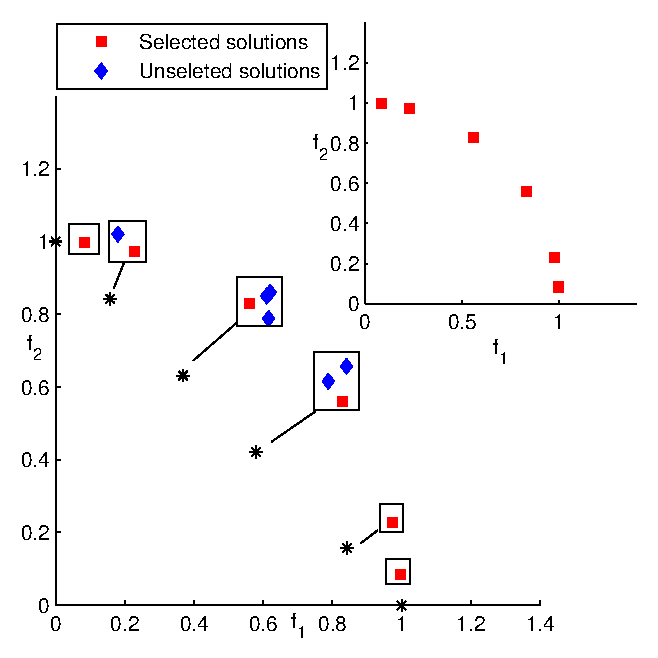
\includegraphics[width=1.4in]{figures/proposedalgorithm/sAlg4.eps}
	}	
	~		
	\subfigure[$k$-means clustering with Euclidean distance measure]
	{
		\label{fig:selectedkmeanseuclidcluster}
		\includegraphics[width=1.4in]{figures/proposedalgorithm/sAlg6.eps}
	}		
	~		
	\subfigure[$k$-means clustering with cosine similarity measure]
	{
		\label{fig:selectedkmeanscosinecluster}
		\includegraphics[width=1.4in]{figures/proposedalgorithm/sAlg7.eps}
	}		
	~
	\subfigure[No clustering i.e., all solutions in one cluster]
	{
		\label{fig:selectedwithoutcluster}
		\includegraphics[width=1.4in]{figures/proposedalgorithm/sAlg5.eps}
	}		
\caption{Solutions are grouped (rectangle box) by different clustering mechanisms. The red squared solutions are the selected solutions obtained by applying fuzzy fitness based environmental selection procedure within each cluster.}

\label{fig:clusteringwfg2}
\end{figure}



\subsection{Adaptive Membership Function}
\label{subsec:membershipFunction}



In this work, we for the first time use the Sigmoid membership function~(Fig.~\ref{fig:sigmoidfunction}) into a
fuzzy based EMO algorithm. This
function is not only monotonically decreasing but also anti-symmetric at mean. We set its growth parameter i.e.,
$\alpha$ in such a way so that it handles the extreme values to some extent 
and work in support of our clustering approach.
The Sigmoid membership function for the $i$-th objective can be defined as 

\begin{equation} \label{eq:SigmoidFunction}
	\gamma_i(f_i({\bf x}^a)-f_i({\bf x}^b))=\frac{1}{1+e^{-\alpha_i((f_i({\bf x}^a)-f_i({\bf x}^b)))}}
\end{equation}

\noindent where mean is set to zero for making the membership function anti-symmetric at that value.

An MOP may or may not have an identical range of values for each objective. To capture this notion, it is better to determine $\alpha_i$ adaptively. We calculate it for each objective at every generation of evolution. The mean objective difference ($\mu_i$) and mean objective  variance ($\sigma_i^2$)
are used to compute $\alpha_i$. We obtain $\mu_i$ and $\sigma_i^2$ using  absolute objective differences of all pairs of solutions.
%The absolute objective difference value between a pair of solutions are same in either order. If we have $n$ solutions then the number of all pair comparisons required is $(n^2-n)/2$. Hence, for the $i$-th objective, the mean $\mu_i$ and variance $\sigma_i^2$ can be defined as  
%
%\vspace{5pt}
%\begin{equation} \label{eq:meanvalue}
%\mu_i=  \frac {2} {(n^2 - n)}  \sum_{{\substack{a = 1}}}^n \sum_{b = a+1}^n  \left|f_i({\bf x}^a) - f_i({\bf x}^b)\right| \\
%\end{equation}
%
%%\noindent The variance of absolute objective differences, $\sigma_i^2$, can be defined as follows.
%
%\begin{eqnarray}\label{eq:varianevalue}
%\sigma_i^2=\frac {1} {\frac{(n^2-n)}{2}-1}\sum_{{\substack{a = 1}}}^n \sum_{b = a+1}^n  \left|\left|f_i({\bf x}^a) - f_i({\bf x}^b) \right|-\mu_i\right|^2
%\end{eqnarray} 
The growth parameter $\alpha_i$  has been defined in such a manner so that the membership value obtained from Eq.~(\ref{eq:SigmoidFunction}) is $0.99$ at
the point $(-\mu_i-\sigma_i)$. We compute  $\alpha_i$ as

\begin{equation} \label{eq:alpha}
	\alpha_i = \frac{\ln{p}-\ln(1-p)}{q_i}
\end{equation}
where $p=0.99$ and $q_i = -\mu_i - \sigma_i$. The way we define $\alpha_i$ is advantageous in three aspects.
% As we define $\alpha_i$ is defined using mean and variance of the objective differences among all pairs of solutions, there are three advantages in such a definition. 
\begin{itemize}
\item Firstly, as $\alpha_i$ is defined based on mean and variance  
instead of maximum or minimum objective difference, inappropriate normalization effect of a significantly large/small objective difference
mentioned in Section~\ref{sec:litrev} will be minimized to some degree.

\item Secondly, if the objectives are in different scales, the corresponding mean and variance of the objective differences will be different
which in turn will produce different $\alpha_i$s i.e., different membership functions.

\item Thirdly, as we cluster the solutions,  all objective differences  in the same cluster
will be small. It ensures that most of the objective differences  will lie in the range between
$-\mu_i-\sigma_i$ and $\mu_i+\sigma_i$. The shape of  membership function indicates that the solutions are evenly discriminable within this range. 
\end{itemize}
In short, the anti-symmetric property and $\alpha_i$'s definition resolve the issues of uneven discrimination ability, objective difference normalization and objective scaling.




\begin{figure}[htbp] 
\centering 
	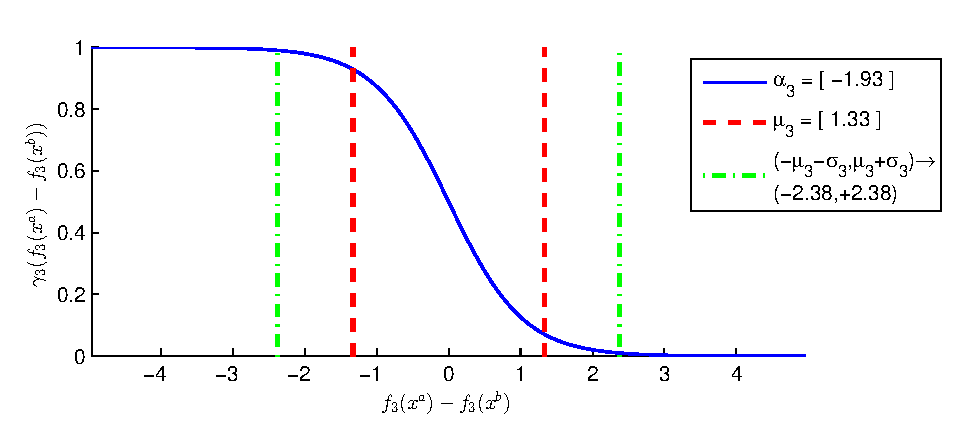
\includegraphics[width=3.3in,height=1.50in]{figures/proposedalgorithm/Nsigmoidfunctionwfg2_3.eps}	
\caption{Sigmoid Membership Function.
This particular case shows the position of mean objective difference value ($\mu_3$) for the third  objective of WFG2 problem obtained from the $250^{th}$ generation of a particular seed.}
\label{fig:sigmoidfunction}
\end{figure}


\subsection{Fuzzy Dominance and Fitness Assignment}
The essence of our fuzzy dominance computation and fitness assignment
is that they are local. We utilize the solutions in the same cluster 
for computing their dominance degrees and assigning their fitness scores. An advantage
of this approach is that there is an opportunity to employ parallelism for 
such computation and assignment. %Parallelism is suitable when evaluation of objective  functions is computationally expensive.
We employ the membership function represented by Eq.~(\ref{eq:SigmoidFunction}) to compute membership
values which in turn are used for obtaining fuzzy dominance among 
all pairs of solutions in each cluster. We use Eqs. (\ref{eq:domi1}) and (\ref{eq:domi2})
for obtaining fuzzy dominance.
 %Eqs. (\ref{eq:domi1}) and (\ref{eq:domi2}) are used for computing dominance degrees. 
%Algorithm~\ref{alg:FuzzyDominaceAlgo} shows the whole procedure of such computations.

%\textbf{The relative fuzzy dominance values, $\phi({\bf x}^a, {\bf x}^b)$ and $\phi({\bf x}^b, {\bf x}^a)$, just express the two product values in the same scale and can effectively differentiate solutions in terms of overall objective wise improvement and provide selection pressure.
%They can be expressed as}
%
%\begin{eqnarray}
%\phi({\bf x}^a, {\bf x}^b)=\frac{dom({\bf x}^a, {\bf x}^b)}{dom({\bf x}^a, {\bf x}^b) + dom({\bf x}^b, {\bf x}^a)} \\
%\phi({\bf x}^b, {\bf x}^a)=\frac{dom({\bf x}^b, {\bf x}^a)}{dom({\bf x}^a, {\bf x}^b) + dom({\bf x}^b, {\bf x}^a)}
%\end{eqnarray}

For assigning fitness to a solution of any cluster, we first compute the relative dominance degrees, $\phi$s, using Eqs. (\ref{eq:re-domi1}) and~(\ref{eq:re-domi2}). Note that the relative dominance degree of any solution $\textbf{x}^a$  in a particular cluster is considered only with respect to all other solutions in that cluster. 
We then add all these degrees and assign it as the solution's fitness 
as represented by~Eq.~(\ref{eq:fitassign}). 

%We then add all these degrees and assign it as the solution's fitness. 
%{\Large We can remove Algorithm 5 and 6}.
%We present this procedure in Algorithm~\ref{alg:FitAssignAlgo}.

\begin{equation} \label{eq:fitassign}
fit(\textbf{x}^a)=  \sum_{b=1, b\neq a}^{b=n} \phi(\textbf{x}^b,\textbf{x}^a)\\
\end{equation}

\noindent Here $n$ is the number of solutions in any cluster. If a solution is least dominated by other solutions of the same
cluster, then its fitness value will be smallest and it will be selected for the next generation.

%
%In absence of clustering, the fuzzy dominance scheme will rank all solutions based on their scalar values. 
%It ensures convergence as the objective wise improvement with respect to all 
%solutions are combined to get such a rank. It, however, will not ensure uniformity in selecting solutions rather
%it introduces bias in selection. For example,  the corner solutions will be preferred for concave surfaces
%while the center ones will be preferred for convex surfaces. Here clustering approach comes into aid for maintaining uniformity among solutions. This issue is further clarified in the following subsection.

\subsection{Environmental Selection}
As mentioned before, $F$-DEA constructs clusters using the evolved solutions as their members and the preferred reference points as their centers. 
 The aim of our environmental selection procedure is to choose solutions for the next generation by considering not only their convergence but also their diversity. 
To achieve these goals, $F$-DEA first sorts the clusters by applying the {\it MinMax} procedure based on the clusters' centers.
This is done to give priority on the distant clusters. The algorithm
then selects the solutions from the sorted clusters in a round robin fashion. For a minimization problem,  a solution having a minimum 
dominance score compared to the remaining  ones of the same cluster is considered for selection. 
%{\bf We use minimum dominance degree to choose solutions}.
It means the selected solution is least dominated by the remaining ones of the same cluster. Giving preference to the distant clusters and selecting the least dominated solutions from them indicates $F$-DEA's emphasis on both diversity and convergence in its environmental selection. 
%Algorithm~\ref{alg:EnvSelectionAlgo} outlines the selection procedure.

To visualize the essence of our reference points based clustering, Fig.~\ref{fig:clusteringwfg2} shows the effect of  reference points based clustering, no clustering, $k$-means clustering with Euclidean distance and  $k$-means clustering with cosine similarity measure. It is evident from this figure that reference points based clustering is able to maintain well both convergence and diversity in selecting solutions for the next generation. In contrast, when no clustering is employed, fuzzy dominance ranks all solutions based on their scalar values and the corner solutions are selected in concave surface due to bias introduced by fuzzy dominance~(Fig.~\ref{fig:selectedwithoutcluster}). 
Diversity maintenance of $k$-means clustering with Euclidean distance (Fig.~\ref{fig:selectedkmeanseuclidcluster}) is better than no clustering (Fig.~\ref{fig:selectedwithoutcluster}) but worse than $k$-means clustering with cosine similarity measure~(Fig.~\ref{fig:selectedkmeanscosinecluster}). To get a further insight of how much contribution we get from reference points based clustering and fuzzy dominance over Pareto dominance, detail experimentation has been conducted and presented in Section~\ref{subsec:impactofrefdominance}.

%\begin{figure*}[htbp] 
%\centering 
%   		
%	\subfigure[Selected solutions using Reference points based clustering]
%	{
%		\label{fig:selectedreferencepointcluster}
%		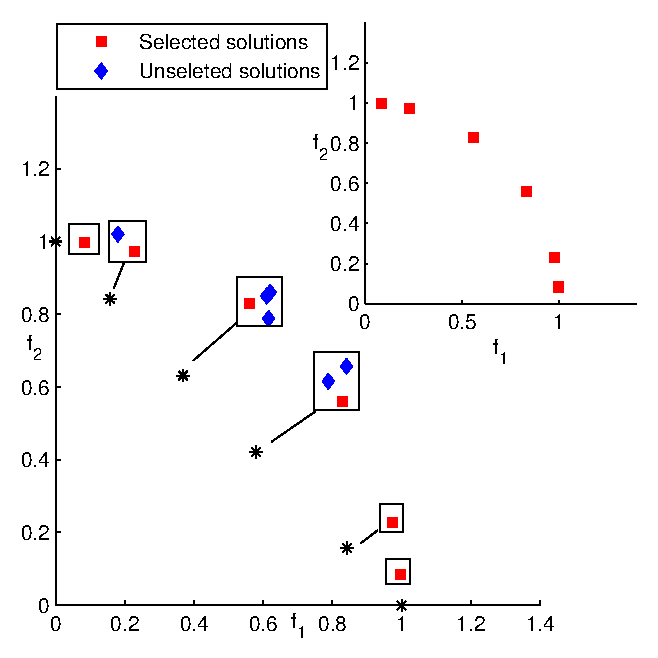
\includegraphics[width=1.50in]{figures/proposedalgorithm/sAlg4.eps}
%	}	
%	~
%	\subfigure[Selected solutions without using any clustering approach]
%	{
%		\label{fig:selectedwithoutcluster}
%		\includegraphics[width=1.50in]{figs/AnalysisFig/writing/sAlg5.eps}
%	}	
%	~		
%	\subfigure[Selected solutions using $k$-means clustering with Euclidean distance measure]
%	{
%		\label{fig:selectedkmeanseuclidcluster}
%		\includegraphics[width=1.50in]{figs/AnalysisFig/writing/sAlg6.eps}
%	}		
%	~		
%	\subfigure[Selected solutions using $k$-means $k$-means clustering with cosine distance measure]
%	{
%		\label{fig:selectedkmeanscosinecluster}
%		\includegraphics[width=1.50in]{figs/AnalysisFig/writing/sAlg7.eps}
%	}		
%	
%\caption{Selected solutions using different selection schemes}
%\label{fig:clusteringwfg2}
%\end{figure*}

\subsection{Computational Complexity}

The basic $F$-DEA algorithm contains seven lines (Algorithm~\ref{alg:completeAlgorithm}). As the first two lines are common in an evolutionary algorithm, the remaining five lines that call five procedures
%~(Algorithms~\ref{alg:prefferedReferencePoint} - \ref{alg:EnvSelectionAlgo})
 actually determine $F$-DEA's complexity.
Algorithm~\ref{alg:prefferedReferencePoint} finds  $p$ preferred reference points from $\left|R^g/R^s\right|$ generated/supplied points and constructs clusters using such points. The overall computation including adaptive normalization (O($mN$)) can be performed with $max(O(mN\left|R^g\right|/\left|R^s\right|,O(mN^2))$ operations.  
The construction of adaptive membership function using mean $\mu$ and  variance $\sigma^2$ requires O$(mN^2)$ operations.%~(Algorithm~\ref{alg:adaptivemembershipfunction})
To calculate $\mu$ and $\sigma^2$ in a single pass, we use the Knuth's running-mean-variance approximation process~\citep{Knuth:1997:ACP:270146}. 
Let the maximum number of solutions in a cluster is $\chi$. As there can be  $p$ different clusters, the time complexity of fitness assignment is at most $O(mp\chi^2)$, including the selection of best solutions
%~(Algorithm~\ref{alg:EnvSelectionAlgo})
  that requires  $max(O(mp^2),O(p\chi))$ or $O(mN^2)$ in the worst case.
%From above analysis, it is clear that $F$-DEA will perform very fast and the only computation burden lies on the active reference points calculation. 
Thus the overall time complexity of $F$-DEA is  $max(O(mN \left|R^g/R^s\right|),O(mN^2))$.
%Parallelism can be used during active reference points calculation and fitness assignment procedures as each cluster is independent with respect to others. In future, we tend to configure this algorithm in a distributed system for complicated problems.

\section{Experimental Studies}
\label{sec:expstudies}

We perform a series of experiments to investigate and compare the optimization capability of our algorithm. Two well known benchmark test suites   WFG~\citep{huband2006review} and 
DTLZ~\citep{deb2005scalable} are utilized for this purpose. The WFG problems are  truly non-linear, non-separable and  multimodal, and they do not have an identical range of values for each objective~\citep{huband2006review}. These characteristics make the WFG problems more challenging than DTLZ ones. To investigate the performance on degenerate problems,
we also include the Rectangle problem~\citep{rectangleproblem} for experimentation.
%In this section, we present experimental details, results, and comparisons with other work.

\subsection{Benchmark Problems}
\label{subsec:testproblems}
%The evaluation and comparison of our method is based on several benchmark problems taken from the WFG and DTLZ test suites. 
The WFG test suite contains nine problems and we choose eight of them for experimentation. We exclude the WFG3 problem because it has a non-degenerate part~\citep{wfgdegenrate} which might create erroneous result during performance evaluation.
To reduce experimentation burden, we choose three  (DTLZ1, DTLZ3 and DTLZ7) out of seven problems of From the DTLZ suite. We  omit
the DTLZ2, DTLZ4 problems from comparative studies as they are relatively easy problems and the DTLZ5, DTLZ6 problems due to their ambiguity in Pareto fronts beyond 3-objective~\citep{huband2006review}.
%Table \ref{table:problems} shows characteristics of the WFG and DTLZ problems.
%We also choose three instances of Rectangle problem.
%Due to page limitation, the experimental results of DTLZ and Rectangle Problems are included as supplementary Materials.

The problems in WFG and DTLZ test suites can be scaled to any number of objectives and decision variables. We consider the number of objectives $m\in\{2, 3, 5, 7, 10, 12, 15, 20, 25\}$. As per recommendation from the WFG Toolkit\footnote{http://www.wfg.csse.uwa.edu.au/toolkit/README.txt}, we set the distance related parameter $l = 20$, the position related parameter $k = 4$  for $m=2$, $k = 2 \times (m-1)$ for  $3 \leq m \leq 10$, and $k = (m-1)$ for  $m >10$.  The number of decision variables, $n$, is set equal to $l + k$. We also follow the suggestions of~\citep{deb2005scalable,deb2014evolutionary} in setting $n$ and $k$ of DTLZ problems. We set $n$ equal to $m + k - 1$ for all DTLZ problems we consider in this work. We set $k = 5$ for DTLZ1, $k = 10$ for DTLZ3 and $k = 20$ for DTLZ7. %{\bf In this study, WFGX-Y refers to the problem WFGX with Y objective. The similar notation is used for the DTLZ problems.}

%
%\begin{table}[]
%	\centering
%	\caption{\textsc{Characteristics of different WFG and DTLZ test Problems.}}
%	\label{table:problems}
%	\begin{tabular}{|c|c|}
%		\thickhline
%		Problem & Features \\ \thickhline
%		WFG1 & Separable, Uni-modal, Biased, Mixed, Scaled \\ \hline
%		WFG2 & \begin{tabular}[c]{@{}c@{}}Nonseparable, Multi-modal\\ Convex, Disconnected, Scaled\end{tabular} \\ \hline
%		%WFG3 & \begin{tabular}[c]{@{}c@{}}Nonseparable, Uni-modal\\ Linear, Degenerate, Scaled\end{tabular} \\ \hline
%		WFG4 & Separable, Multi-modal, Concave, Scaled \\ \hline
%		WFG5 & Separable, Deceptive, Concave, Scaled \\ \hline
%		WFG6 & Nonseparable, Uni-modal, Concave, Scaled \\ \hline
%		WFG7 & Separable, Uni-modal, Biased, Concave, Scaled \\ \hline
%		WFG8 & Nonseparable, Uni-modal, Biased Concave, Scaled \\ \hline
%		WFG9 & \begin{tabular}[c]{@{}c@{}}Nonseparable, Multi-modal, Deceptive\\  Biased, Concave, Scaled\end{tabular} \\ \hline
%		DTLZ1 & Separable, Multi-modal, Linear \\ \hline
%		DTLZ2 & Separable, Uni-modal, Concave \\ \hline
%		DTLZ3 & Separable, Multi-modal, Concave \\ \hline
%		DTLZ4 & Separable, Uni-modal, Biased, Concave \\ \hline
%		DTLZ7 & Multi-modal, Disconnected \\ \thickhline
%	\end{tabular}
%\end{table}

\subsection{Performance metrics}
\label{subsec:peformancemetrics}

The performance of any evolutionary  algorithm for an MOP is usually measured from two aspects: convergence and diversity. Inverse generalization distance (IGD)~\citep{zitzler2003performance} and hypervolume (HV)~\citep{zitzler1999multiobjective} are two performance metrics that capture in one scalar both convergence and diversity. 
To calculate IGD, a well uniform sample set of true Pareto front is required. It is, however, challenging to get such a set for an increasing number of objectives~\citep{xinyao6883177}. %Deb and Jain~\citep{deb2014evolutionary} recently introduced a direct procedure for calculating IGD based on the reference points, where for each reference direction we can exactly locate the intersecting point of a known true Pareto front. 

%The other performance metric HV is suitable for algorithms that search the Pareto front in the sparsely distributed objective space.
The other performance metric HV has nicer mathematical properties  and is the only quality measure known to be strictly Pareto-compliant~\citep{zitzler2003performance}.
These good features make HV a fair indicator for comparing different algorithms. For a non-dominated solution set $A$ obtained in final generation by an algorithm, HV is calculated with respect to a reference point {\bf r}.
%HV of $A$ with respect to {\bf r} is the volume of region dominated by $A$ and bounded by {\bf r}.
%
%\begin{equation}
%HV(A,{\bf r}) = volume(\bigcup\limits_{f\in A}[f_1,r_1]\times\cdots\times[f_m,r_m])
%\label{eq:hv}
%\end{equation}
%\noindent The choice of {\bf r} is crucial in computing HV and 
\noindent It has been known that choosing {\bf r} slightly larger than the nadir point, ${\bf z}^{nad}$, is suitable~\citep{ishibuchi2010many}. In our experiments, we set {\bf r} to $1.1{\bf z}^{nad}$, which can be analytically obtained or approximated~\citep{huband2006review}. 
%The Pareto front of WFG4-WFG9 is part of a hyper-ellipse with radii $R_i=2\times i$ ( $i = 1, 2,\cdots,m$) and has a regular geometry~\citep{piceag,huband2006review}. It of DTLZ1-DTLZ4 also has a regular shape. As the Pareto fronts of WFG1 (mixed), WFG2 (disconnected) and DTLZ7 (disconnected) do not have a regular geometry, we obtain ${\bf z}^{nad}$ for these problems by an using an approximation procedure. 
Following \citep{wagner2007pareto}, the points which do not dominate {\bf r} are discarded in computing HV. 
%For the problems having Pareto fronts with differently scaled objective values, we first normalize the objective values of the points in $A$ and the reference point ${\bf r}$ using ${\bf z}^{nad}$ and ${\bf z}^{*}$ before computing HV. Here  ${\bf z}^{*}$  indicates the optimal objective value, which is $0$ for all adopted problems we consider in this study. Thus the computed HV for an $m$-objective problem would be between $0$ and $1.1^m - V_m$, where $V_m$ is hypervolume of the region enclosed by the normalized Pareto front and coordinate axes. 
We use exact HV calculation for problems with objective less than $5$ and the Monte Carlo based fast HV approximation algorithm~\citep{bader2011hype} with $10,00,000$ sampling points for others. %The large number of sampling points is considered here to ensure accuracy in computing HV. 

In experimental studies, we have used HV, IGD and visualization figures to evaluate performances of the algorithms.

\subsection{ Other Algorithms in Comparison}

There exists a few fuzzy dominance based EMO algorithms in the literature. FD-NSGAII~\citep{he2014fuzzy} is one such algorithm, which has been found
better than other similar algorithms. We thus select  FD-NSGAII for comparison. We also choose NSGAIII~\citep{deb2014evolutionary} for comparison because it exhibits superior performance compared to several well-known algorithms.
Decomposition based algorithm MOEA/D~\citep{zhang2007moea} with weighted Tchebycheff approach has been chosen as a representative of decomposition, aggregation and reference weights/points based approach. 
%Although a new version of MOEA/D (e.g.~MOEA/D-DE~\citep{li2009multiobjective}) with differential evolution has been proposed to deal with complicated Pareto surfaces, it has been found to be shown poor performance in MaOPs~\citep{deb2014evolutionary}. 
We choose a variant of SDE~\citep{sdealgorithm}, SPEA2+SDE, for comparison. This particular variant shows the best overall performance among its other variants~\citep{sdealgorithm}.
%, NSGA-II+SDE, SPEA2+SDE and PESA-II+SDE~\citep{sdealgorithm}.
Preference based co-evolutionary algorithm (PICEAg)~\citep{piceag} and HypE~\citep{bader2011hype}, an indicator based algorithm,  are also
chosen for comparison. 
%HypE adopts Monte Carlo simulation to approximate exact hypervolume.
%Its core idea is that only the rankings of the solutions induced by the hypervolume indicator are important, while the actual indicator values are not.
%All the aforementioned algorithms cover standard approaches for solving MaOPs. 

%Due to fuzzy nature of our algorithm and being a reference points based algorithm we will focus our analysis with FD-NSGAII and NSGAIII for further investigation.



\subsection{Parameter Setting}
\label{subsec:parametersettings}

The population size $N$ of NSGAIII cannot be arbitrarily specified, rather it has to be set equal to the number of reference points. The procedure employed for generating such points uses a division parameter $\lambda$ that determines this number. Although our algorithm uses reference points, it does not put any constraint in choosing $N$. 
Table~\ref{table:popsize} shows $\lambda$ of NSGAIII and $F$-DEA, the weights $Z$ of MOEA/D and the number of goals $G$ for PICEAg. To make a fair comparison, the population size is set same for all competing algorithms.% (Table~\ref{table:popsize}) and it is chosen based on  NSGAIII.  

All competing algorithms employ simulated binary crossover and polynomial mutation for generating offspring. The crossover and mutation probabilities are set to 1 and 1/$n$, respectively. We also use the same mutation distribution index i.e., 20 for these algorithms.  The crossover distribution index is set to 30 for $F$-DEA and NSGAIII, 20 for SDE, and 15 for HypE, MOEA/D, FD-NSGAII, and PICEAg. 
Beside the general and common parameters, there are some specific parameters for competing algorithms. The parameter $p$ of $F$-DEA
is set equal to $N$. The bound of reference point and the number of sampling points
used in HypE~\citep{bader2011hype} has  been set to $200$ and $10,000$, respectively. In MOEA/D~\citep{zhang2007moea,li2009multiobjective}, the neighborhood size, $T$, is chosen $5\%$ of the population and the maximum number of population slots, $\eta_r$,  has been chosen $1\%$ of $T$. The fuzzy ranking threshold parameter $\beta$
of FD-NSGAII~\citep{he2014fuzzy} has been set to $0.50$. In SDE~\citep{sdealgorithm}, the archive is set equal to population size, $N$.
The number of goals $G$ used in PICEAg~\citep{piceag} is set to $m \times 100$.

%	\item FD-NSGAII~\citep{he2014fuzzy}: The fuzzy ranking threshold parameter $\beta$ has been set to $0.50$. 
%	\item MOEA/D~\citep{zhang2007moea,li2009multiobjective}: The neighborhood size, $T$, is chosen $5\%$ of the population and the maximum number of population slots, $\eta_r$,  has been chosen $1\%$ of $T$.
%	\item FD-NSGAII~\citep{he2014fuzzy}: The fuzzy ranking threshold parameter $\beta$ has been set to $0.50$. 

%\begin{enumerate}
%	\item $F$-DEA: The division number, $\lambda$, of the Das and Dennis's procedure~\citep{das1998normal} used in $F$-DEA is shown in Table~\ref{table:popsize} and 
%	$p$ is set equal to $N$.
%	\item HypE~\citep{bader2011hype}: The bound of reference point  and the number of sampling points have  been set to $200$ and $10,000$, respectively.
%	\item MOEA/D~\citep{zhang2007moea,li2009multiobjective}: The neighborhood size, $T$, is chosen $5\%$ of the population and the maximum number of population slots, $\eta_r$,  has been chosen $1\%$ of $T$.
%	\item FD-NSGAII~\citep{he2014fuzzy}: The fuzzy ranking threshold parameter $\beta$ has been set to $0.50$. 
%	\item NSGAIII~\citep{deb2014evolutionary}: The division number, $\lambda$, of the Das and Dennis's procedure~\citep{das1998normal} used in  NSGAIII is shown in Table~\ref{table:popsize}.
%	\item SDE~\citep{sdealgorithm}: the archive is set equal to population size, $N$.
%	\item PICEAg~\citep{piceag}: The number of goal $G$ is set to $m \times 100$.
%	
%\end{enumerate}

\begin{table}[]
	\centering
	\caption{\textsc{Population Size $N$, number of divisions $\lambda$ used in NSGAII~\citep{deb2002fast} and $F$-DEA, number of weight vectors $Z$ used in MOEA/D~\citep{zhang2007moea}} and goals in PICEAg~\citep{piceag} for different objectives}
	\label{table:popsize}
%\setlength{\tabcolsep}{2pt}
\renewcommand{\arraystretch}{1.1}
\begin{adjustbox}{width=0.50\textwidth,center}
\begin{tabular}{c|c|c|c|c|c}
\thickhline
\multicolumn{1}{c|}{\multirow{2}{*}{\begin{tabular}[c]{@{}l@{}}Obj. No.\\ ($m$)\end{tabular}}} & \multicolumn{1}{c|}{\multirow{2}{*}{\begin{tabular}[c]{@{}l@{}}$N$ used in\\ all algorithms\end{tabular}}} & \multicolumn{2}{c|}{$\lambda$ used in} & \multicolumn{1}{c|}{\multirow{2}{*}{\begin{tabular}[c]{@{}c@{}}$Z$ used in\\ MOEA/D\end{tabular}}} & \multicolumn{1}{c}{\multirow{2}{*}{\begin{tabular}[c]{@{}c@{}}$G$ used in\\ PICEAg\end{tabular}}} \\ \cline{3-4}
\multicolumn{1}{c|}{} & \multicolumn{1}{c|}{} & \multicolumn{1}{c|}{NSGAIII} & \multicolumn{1}{c|}{F-DEA} & \multicolumn{1}{c|}{} & \multicolumn{1}{c}{} \\\thickhline
2 & 204 & 200 & 2000 & 20400 & 200 \\
3 & 204 & 18 & 100 & 20400 & 300 \\
5 & 212 & 6 & 30 & 21200 & 500 \\
7 & 212 & 4 & 13 & 21200 & 700 \\
10 & 220 & 3 & 9 & 22000 & 1000 \\
12 & 160 & 2, 2 & 7 & 16000 & 1200 \\
15 & 240 & 2, 2 & 6 & 24000 & 1500 \\
20 & 212 & 2 & 5 & 21200 & 2000 \\
25 & 328 & 2 & 4 & 32800 & 2500 \\ \thickhline
\end{tabular}
\end{adjustbox}
\end{table}


Each algorithm is run independently with 20 different seeds for each problem instance. We set the termination criterion to $250$ generations for each run. The Wilcoxon rank-sum test~\citep{haynes2013wilcoxon}
%, which is equivalent to the Mann–Whitney $U$ test~\citep{mann1947test} (MATLAB implementation\footnote{http://www.mathworks.com/help/stats/ranksum.html})
 with a $5\%$-significance level is used while comparing two algorithms on any problem instance over 20 runs. For reducing Type-I error in pairwise testing, {\v{S}}id{\'a}k corrections~\citep{abdi2007bonferonni} are also employed.
$F$-DEA has been implemented by the authors in~\textit{JMetal\footnote{www.jmetal.org\label{jmetal}}} framework and it's source code is available online\footnote{https://github.com/siddhartha047/FDEA}. HypE and MOEA/D  from MOEA framework\footnote{www.moeaframework.org\label{moeaframework}}. We use
a C++ implementation\footnote{http://web.ntnu.edu.tw/~tcchiang/publications/nsga3cpp/nsga3cpp.htm\label{nsgaiiilink}} for NSGAIII. FD-NSGAII has been implemented by the authors from~\citep{he2014fuzzy} in~\textit{JMetal} framework. The source codes of SDE and PICEAg algorithms are received from the authors of the respective algorithms. The true Pareto front of the WFG problems is generated using the ~\textit{WFG-Toolkit}~\footnote{http://www.wfg.csse.uwa.edu.au/toolkit/}.
The uniform Pareto front of DTLZ1, DTLZ3 is generated from NSGAIII implementation tools\footref{nsgaiiilink}.
%For the DTLZ7 problems, the Pareto front is generated using \textit{MOEAFramework}~\footref{moeaframework}. 
All algorithms were run on Intel $2.40$GHz core i5 processor with 4GB RAM. The performance evaluation and visualization codes are shared in \textit{Github}~\footnote{https://github.com/siddhartha047/MOEAevaluation-plot}.



\subsection{Experiment on WFG Problems}
This section presents evaluation and comparison of our $F$-DEA and six other algorithms on eight WFG problems with 2-, 3-, 5-, 7-, 10-,  12-, 15-,  20- and 25-objective.
Table~\ref{table:hypewfg1} shows the average HV with standard deviation and ranks of different algorithms obtained by the Wilcoxon rank-sum test based on HVs of 20 independent runs. The lower a rank is, the better an algorithm is. 


%For a particular problem, the performance score is a count that indicates the number of times the algorithm is significantly beaten by  the competing algorithms based the Wilcoxon rank-sum test. If there are $h$ algorithms,  the lowest score could be 0 (none found better) and the highest one could be $h-1$ (all the competing algorithms are better). The lower the score is, the better the algorithm is. The detail results of these problems are given in appendix for brevity.
		
\subsubsection{WFG1 Problem}

The WFG1 problem has most transformation functions among the other problems of the same suite. Hence, it is difficult to maintain diversity with sufficient convergence for this problem
% and algorithms that stress over diversity will fail to achieve convergence. 
 $F$-DEA exhibited the best performance among all competing algorithms from 2-objective to 25-objective. 
%PICEAg, NSGAIII, SDE were the close competitors for a lower number of objectives. %As the number of objective increases, FD-NSGAII secured the second position and exhibited better results compared to others. 

\subsubsection{WFG2 Problem}
%This is the only disconnected problem in the WFG test suite. %To achieve good performance, it is necessary for an algorithm to distribute the obtained solutions in all the disconnected regions. 
%FD-NSGAII exhibited the worst performance on this problem with nine different objectives we considered in this work. 
NSGAIII was the top performer in 2-objective, while PICEAg and SDE were the top two performers from 3-objective to 25-objective. $F$-DEA secured overall the third position  and showed very competitive performance with respect to average HVs achieved by the top performers.
 
%\input{hypewfg2}

%\subsubsection{WFG3 Problem}
%Table~\ref{table:hypewfg3} shows the  results of different algorithms on the degenerative problem WFG3. 
%\sout{The proposed $F$-DEA showed a very similar performance with NSGAIII for this problem with a lower number of objectives i.e., 2-objective to 7-objective, but it exhibited a superior performance for  the higher number of objectives i.e., 10-objective to 20-objective. In terms of average rank, $F$-DEA was the best performer and GDE3 was the worst performer.}
%\input{hypewfg3}

\subsubsection{WFG4 Problem}
%The results of $F$-DEA and other algorithms for the concave multi-modal problem WFG4 are given in \sout{Table~\ref{table:hypewfg4}.}
%\sout{$F$-DEA outperformed all other algorithms on this problem with 3-objective to $20$-objective and secured the second position on the $2$-objective. NSGAIII and MOEA/D were the closest competitors and they secured the second and third positions, respectively.} %WFG4 is a concave multi-modal problem, the convergence property of FD-NSGAII moves solution to one side in high dimension which can be also realized from the parallel coordinate plot of WFG4\_15 plot in Fig.~\ref{} and makes it the worst performer in terms of HV due to lack of diversity.  
%\input{hypewfg4}

For a smaller number of objectives, SDE and PICEAg were the two top performing algorithms while $F$-DEA showed competitive performance.  $F$-DEA, however, tied with SDE in $7$-objective and outperformed all other competing algorithms from $10$-objective to $25$-objective. %These results indicate that the performance of $F$-DEA improves as the number of objectives increases.

\subsubsection{WFG5 Problem}
%\sout{An important aspect of this problem is its deceptive nature, which challenges the ability of an algorithm to find good quality solutions. Our $F$-DEA handled the challenge successfully and outperformed all competing algorithms from 3-objective to 20-objective. For the 2-objective, NSGAIII secured the first position and $F$-DEA the second position.} %Table~\ref{table:hypewfg5} summarizes the results. 

An important aspect of this problem is its deceptive nature, which challenges the ability of an algorithm to find good quality solutions. $F$-DEA handled the challenge successfully and outperformed all competing algorithms from 15-objective to 25-objective. 
%From 7-objective to 12-objective, $F$-DEA, SDE and PICEAg were top performers. Our algorithm also showed competitive performance for $2$-, $3$- and $5$-objective. %Table~\ref{table:hypewfg5} summarizes the results. 

%\input{hypewfg5}

\subsubsection{WFG6 Problem}
%Table~\ref{table:hypewfg6}} shows the performances of the competing algorithms on the non-separable reduced problem WFG6. 
%\sout{$F$-DEA was the top performer in almost all cases of the non-separable reduced problem WFG6. There was only one instance (WFG6 with 2-objective) where our algorithm shared the top position with GDE3. In terms of average rank, our algorithm was far better with respect to the other algorithms. While the average rank of $F$-DEA  was 1.0625, MOEA/D, the best competitor of $F$-DEA for this problem, achieved an average rank of 2.5625.}

$F$-DEA was the top performer from $12$-objective  to $25$-objective of the non-separable reduced problem, WFG6. 
The proposed algorithm shared the top position with SDE and PICEAg for $2$-objective  and with PICEAg for 10-objective.
%For other objectives, $F$-DEA showed competitive performance with the top performers.

%\input{hypewfg6}

\subsubsection{WFG7 Problem}
%\sout{This is a separable unimodal problem. Similar to the previous cases, $F$-DEA showed better performance with an increasing number of objectives. More specifically, it outperformed all other algorithms on this problem with  3-objective to 20-objective. It was beaten by only NSGAIII with 2-objective and secured the second position jointly with GDE3.} %We present the results of competing algorithms in \sout{Table~\ref{table:hypewfg6}}. 
%\input{hypewfg7}
%Table \ref{table:hypewfg7} shows the HV of the compared algorithms on WFG7. WFG7 is a separable unimodal problem. $F$-DEA outperforms all others in $3$ to $20$ problem instances. In $2$ objective instance NSGAIII ranks $1$ and $F$-DEA, GDE3 tie with rank $2.5$. FD-NSGAII gives worst performance due to lack of diversity.

This is a separable unimodal problem. $F$-DEA showed better performance with an increasing number of objectives.
For example, it outperformed all other algorithms from 
15-objective to 25-objective.
% and showed competitive performance with SDE, PICEAg and NSGAIII for a smaller number of objectives.  

\subsubsection{WFG8 Problem}
%In \sout{Table \ref{table:hypewfg8}}, the performances of the competing algorithms on the non-separable problem WFG8 are presented. 
%\sout{Our $F$-DEA outperformed the others not only in a larger number of objectives (5-objective to 20-objective) of the non-separable problem WFG8  but also in a smaller number of objectives (2-objective and 3-objective). The average rank of $F$-DEA is far better (1.0 vs 2.5) than the second best performer NSGAIII.}

SDE, PICEAg and $F$-DEA were the top performing algorithms with close average HV values for this 
non-separable problem.
SDE was the top performer for 2-, 3- and 20-objective, PICEAg for 5- and 10-objective,
and $F$-DEA for $15$- and $25$-objective. 
%$F$-DEA together with SDE became the top performer for the $12$-objective and it secured the second position for the $2$-, $7$-, $10$ and $20$-objective with relatively close average HV values.

%\input{hypewfg8}
\subsubsection{WFG9 Problem}
%\sout{Table~\ref{table:hypewfg9}} shows the results of all competing algorithms. 
%\sout{It is clear from the table that  $F$-DEA was the best among all algorithms for this problem with 7-objective to 20-objective. For the 3-objective and 5-objective, our $F$-DEA and NSGAIII showed similar performance and they both outperformed other algorithms.  NSGAIII, however, outperformed $F$-DEA for this problem with 2-objective. }

This is a non-separable deceptive problem for which NSGAIII and SDE were two top performers for
2-, 3- and 5-objective.  As the number objective increases, the performance of $F$-DEA enhanced and shared the 
top position with  SDE, PICEAg for the $7$- and $10$-objective. However, $F$-DEA outperformed all other algorithms from 12-objective to 25-objective.

\begin{table*}[]
\centering
\caption{Average HV of different algorithms on eight WFG problems over 20 independent runs. The best result based on the Wilcoxon rank sum test with a significance level of $0.05$ is marked in bold-face. The rank of a particular algorithm is shown in bracket.}
\label{table:hypewfg1}
%\setlength{\tabcolsep}{2pt}
\renewcommand{\arraystretch}{1.1}
%\resizebox{\textwidth}{!}{
\begin{adjustbox}{width=1.0\textwidth,center}
\begin{tabular}{lllllllll}
\thickhline
Prob. & \multicolumn{1}{c}{\textit{m}} & \multicolumn{1}{c}{HYPE} & \multicolumn{1}{c}{MOEA/D} & \multicolumn{1}{c}{FD-NSGAII} & \multicolumn{1}{c}{SDE}                       & \multicolumn{1}{c}{NSGAIII}          & \multicolumn{1}{c}{PICEA-g}            & \multicolumn{1}{c}{F-DEA}   \\\thickhline
wfg1  & 2                              & 0.0970$\pm$0.0257(6)         & 0.1467$\pm$0.0264(5)          & 0.0495$\pm$0.0214(7)              & 0.2324$\pm$0.0434(4)                              & \textbf{0.3333$\pm$0.0689(1.5)}          & 0.3233$\pm$0.0037(3)                       & \textbf{0.3438$\pm$0.0371(1.5)} \\
      & 3                              & 0.2968$\pm$0.0248(7)         & 0.4042$\pm$0.0485(5)          & 0.3959$\pm$0.0226(5)              & 0.5614$\pm$0.0497(2.5)                            & 0.4094$\pm$0.0396(5)                     & 0.5689$\pm$0.0052(2.5)                     & \textbf{0.6120$\pm$0.0413(1)}   \\
      & 5                              & 0.3515$\pm$0.0347(7)         & 0.5187$\pm$0.0246(5)          & 0.5979$\pm$0.0474(3)              & 0.5622$\pm$0.0232(4)                              & 0.4065$\pm$0.0732(6)                     & 0.7117$\pm$0.0114(2)                       & \textbf{0.7516$\pm$0.0337(1)}   \\
      & 7                              & 0.4164$\pm$0.0279(7)         & 0.5985$\pm$0.0402(5)          & 0.8524$\pm$0.0531(2.5)            & 0.7058$\pm$0.0256(4)                              & 0.4824$\pm$0.0275(6)                     & 0.8429$\pm$0.0297(2.5)                     & \textbf{0.9058$\pm$0.0560(1)}   \\
      & 10                             & 0.6005$\pm$0.0225(6)         & 0.8432$\pm$0.0692(5)          & 1.2047$\pm$0.0754(2)              & 0.9937$\pm$0.0418(4)                              & 0.3671$\pm$0.0924(7)                     & 1.0310$\pm$0.0307(3)                       & \textbf{1.4206$\pm$0.0684(1)}   \\
      & 12                             & 0.6543$\pm$0.0292(6)         & 0.8989$\pm$0.0669(5)          & 1.3867$\pm$0.1012(2)              & 1.1189$\pm$0.0517(4)                              & 0.2839$\pm$0.0633(7)                     & 1.2233$\pm$0.0310(3)                       & \textbf{1.6017$\pm$0.1296(1)}   \\
      & 15                             & 0.8732$\pm$0.0501(6)         & 1.2230$\pm$0.0545(5)          & 2.1247$\pm$0.1903(2)              & 1.6596$\pm$0.0671(3)                              & 0.4128$\pm$0.1145(7)                     & 1.5930$\pm$0.0473(4)                       & \textbf{2.3314$\pm$0.1024(1)}   \\
      & 20                             & 1.2481$\pm$0.0439(6)         & 1.6443$\pm$0.1007(5)          & \textbf{3.4625$\pm$0.3626(1.5)}   & 2.7029$\pm$0.1280(3)                              & 0.3940$\pm$0.1587(7)                     & 2.5527$\pm$0.0635(4)                       & \textbf{3.5738$\pm$0.2874(1.5)} \\
      & 25                             & 2.1095$\pm$0.1037(6)         & 2.4165$\pm$0.1568(5)          & 6.6621$\pm$0.3718(2)              & 2.8201$\pm$0.0539(4)                              & 1.8261$\pm$0.2503(7)                     & 4.0829$\pm$0.0980(3)                       & \textbf{7.1479$\pm$0.4528(1)}  \\\thickhline
wfg2  & 2                              & 0.6806$\pm$0.0149(5.5)       & 0.6820$\pm$0.0183(5.5)        & 0.3459$\pm$0.0572(7)              & 0.7407$\pm$0.0054(2)                              & \textbf{0.7452$\pm$0.0087(1)}            & 0.7406$\pm$0.0091(3)                       & 0.7363$\pm$0.0064(4)            \\
      & 3                              & 0.9702$\pm$0.0767(5.5)       & 1.0575$\pm$0.0972(5.5)        & 0.3862$\pm$0.0656(7)              & 1.2207$\pm$0.0581(2)                              & 1.1573$\pm$0.0929(3.5)                   & \textbf{1.2450$\pm$0.0022(1)}              & 1.2119$\pm$0.0418(3.5)          \\
      & 5                              & 1.3316$\pm$0.1315(4.5)       & 1.3283$\pm$0.1175(6)          & 0.4409$\pm$0.0009(7)              & 1.5401$\pm$0.0840(2)                              & 1.3872$\pm$0.1229(4.5)                   & \textbf{1.5546$\pm$0.1049(1)}              & 1.5277$\pm$0.0838(3)            \\
      & 7                              & 1.6032$\pm$0.1593(5.5)       & 1.4962$\pm$0.1489(5.5)        & 0.5498$\pm$0.0678(7)              & 1.8686$\pm$0.1022(2)                              & 1.6951$\pm$0.1574(4)                     & \textbf{1.8875$\pm$0.1285(1)}              & 1.8347$\pm$0.1241(3)            \\
      & 10                             & 2.2659$\pm$0.1715(4.5)       & 2.1991$\pm$0.1021(6)          & 0.5655$\pm$0.2030(7)              & 2.5531$\pm$0.0064(2)                              & 2.3060$\pm$0.0507(4.5)                   & \textbf{2.5889$\pm$0.0018(1)}              & 2.5280$\pm$0.0097(3)            \\
      & 12                             & 2.6969$\pm$0.0885(4.5)       & 2.5541$\pm$0.1337(6)          & 0.6473$\pm$0.2821(7)              & 3.0745$\pm$0.0166(2)                              & 2.6757$\pm$0.0975(4.5)                   & \textbf{3.1266$\pm$0.0034(1)}              & 3.0375$\pm$0.0228(3)            \\
      & 15                             & 3.7255$\pm$0.1172(4)         & 3.5520$\pm$0.1362(5.5)        & 0.8039$\pm$0.3350(7)              & 4.1263$\pm$0.0084(2)                              & 3.5388$\pm$0.0700(5.5)                   & \textbf{4.1692$\pm$0.0022(1)}              & 4.0798$\pm$0.0196(3)            \\
      & 20                             & 5.7851$\pm$0.4480(4.5)       & 5.6843$\pm$0.2581(4.5)        & 1.2816$\pm$0.6254(7)              & 6.6467$\pm$0.0169(2)                              & 4.0451$\pm$0.7806(6)                     & \textbf{6.7064$\pm$0.0094(1)}              & 6.5645$\pm$0.0299(3)            \\
      & 25                             & 9.6551$\pm$0.3095(4.5)       & 9.1922$\pm$0.3394(6)          & 2.2394$\pm$0.9957(7)              & 10.6314$\pm$0.0470(2.5)                           & 8.9972$\pm$1.8322(4.5)                   & \textbf{10.8188$\pm$0.0074(1)}             & 10.6293$\pm$0.0517(2.5)         \\\thickhline
wfg4  & 2                              & 0.3946$\pm$0.0041(6)         & 0.4058$\pm$0.0044(5)          & 0.1278$\pm$0.0377(7)              & \textbf{0.4184$\pm$0.0010(1.5)}                   & \textbf{0.4182$\pm$0.0010(1.5)}          & 0.4143$\pm$0.0014(4)                       & 0.4172$\pm$0.0006(3)            \\
      & 3                              & 0.6447$\pm$0.0203(6)         & 0.6697$\pm$0.0115(5)          & 0.1220$\pm$0.0053(7)              & \textbf{0.7501$\pm$0.0028(1)}                     & 0.7096$\pm$0.0038(4)                     & 0.7432$\pm$0.0021(2)                       & 0.7321$\pm$0.0024(3)            \\
      & 5                              & 0.9151$\pm$0.0969(6)         & 1.0343$\pm$0.0251(5)          & 0.2472$\pm$0.0915(7)              & 1.2164$\pm$0.0083(2.5)                            & 1.0503$\pm$0.0134(4)                     & \textbf{1.2475$\pm$0.0262(1)}              & 1.2220$\pm$0.0083(2.5)          \\
      & 7                              & 1.1010$\pm$0.1397(6)         & 1.3328$\pm$0.0423(4)          & 0.3230$\pm$0.1273(7)              & \textbf{1.6016$\pm$0.0149(1.5)}                   & 1.3015$\pm$0.0559(4)                     & 1.3295$\pm$0.0982(4)                       & \textbf{1.6127$\pm$0.0221(1.5)} \\
      & 10                             & 1.5518$\pm$0.1823(6)         & 2.0844$\pm$0.0399(4.5)        & 0.4548$\pm$0.1907(7)              & 2.3121$\pm$0.0292(2)                              & 2.0664$\pm$0.0923(4.5)                   & 2.1635$\pm$0.0753(3)                       & \textbf{2.3892$\pm$0.0111(1)}   \\
      & 12                             & 1.6225$\pm$0.2620(6)         & 2.4331$\pm$0.1179(3)          & 0.4192$\pm$0.1924(7)              & 2.7870$\pm$0.0416(2)                              & 1.9808$\pm$0.0874(5)                     & 2.3082$\pm$0.1245(4)                       & \textbf{2.8607$\pm$0.0273(1)}   \\
      & 15                             & 2.3364$\pm$0.3730(6)         & 3.4223$\pm$0.0955(3.5)        & 0.6341$\pm$0.2520(7)              & 3.7551$\pm$0.0348(2)                              & 2.7353$\pm$0.1271(5)                     & 3.3657$\pm$0.1431(3.5)                     & \textbf{3.9442$\pm$0.0311(1)}   \\
      & 20                             & 3.6517$\pm$0.3742(6)         & 5.2892$\pm$0.1486(3.5)        & 0.7661$\pm$0.2789(7)              & 5.9939$\pm$0.2018(2)                              & 4.0528$\pm$0.2925(5)                     & \multicolumn{1}{c}{5.1166$\pm$0.3164(3.5)} & \textbf{6.3855$\pm$0.0460(1)}   \\
      & 25                             & 7.4075$\pm$0.6866(6)         & 8.8991$\pm$0.1289(3.5)        & 1.1546$\pm$0.1966(7)              & 9.4890$\pm$0.4354(2)                              & 8.2805$\pm$0.4261(5)                     & \multicolumn{1}{c}{8.7945$\pm$0.5704(3.5)} & \textbf{10.5396$\pm$0.0492(1)}  \\\thickhline
wfg5  & 2                              & 0.3243$\pm$0.0122(6)         & 0.3603$\pm$0.0068(5)          & 0.0861$\pm$0.0202(7)              & \textbf{0.3743$\pm$0.0005(1.5)}                   & 0.3740$\pm$0.0006(3.5)                   & \textbf{0.3741$\pm$0.0009(1.5)}            & 0.3737$\pm$0.0008(3.5)          \\
      & 3                              & 0.5445$\pm$0.0262(6)         & 0.6056$\pm$0.0145(5)          & 0.1142$\pm$0.0305(7)              & \textbf{0.7010$\pm$0.0035(1)}                     & 0.6648$\pm$0.0056(4)                     & 0.6966$\pm$0.0033(2)                       & 0.6882$\pm$0.0022(3)            \\
      & 5                              & 0.8947$\pm$0.0602(6)         & 0.9683$\pm$0.0248(5)          & 0.1278$\pm$0.0006(7)              & 1.1715$\pm$0.0074(3)                              & 0.9993$\pm$0.0119(4)                     & \textbf{1.1854$\pm$0.0038(1)}              & 1.1800$\pm$0.0073(2)            \\
      & 7                              & 1.0418$\pm$0.1275(6)         & 1.2624$\pm$0.0405(4.5)        & 0.1554$\pm$0.0003(7)              & 1.5562$\pm$0.0097(3)                              & 1.2482$\pm$0.0517(4.5)                   & \textbf{1.5814$\pm$0.0173(1.5)}            & \textbf{1.5809$\pm$0.0085(1.5)} \\
      & 10                             & 1.4758$\pm$0.1146(6)         & 1.9581$\pm$0.0466(4)          & 0.2064$\pm$0.0005(7)              & 2.2843$\pm$0.0079(2)                              & 1.8706$\pm$0.0613(5)                     & 2.1577$\pm$0.0755(3)                       & \textbf{2.2964$\pm$0.0062(1)}   \\
      & 12                             & 1.6040$\pm$0.1641(6)         & 2.2598$\pm$0.0914(4)          & 0.2487$\pm$0.0005(7)              & \textbf{2.7525$\pm$0.0127(1.5)}                   & 2.0394$\pm$0.1186(5)                     & 2.3688$\pm$0.0823(3)                       & \textbf{2.7670$\pm$0.0236(1.5)} \\
      & 15                             & 2.4435$\pm$0.1978(6)         & 3.2303$\pm$0.0904(4)          & 0.3316$\pm$0.0016(7)              & 3.6807$\pm$0.0185(2)                              & 2.7944$\pm$0.1447(5)                     & 3.3723$\pm$0.0774(3)                       & \textbf{3.7649$\pm$0.0091(1)}   \\
      & 20                             & 3.6012$\pm$0.4559(6)         & 5.0711$\pm$0.2051(3.5)        & 0.5312$\pm$0.0011(7)              & 5.9066$\pm$0.0244(2)                              & 4.5393$\pm$0.3738(5)                     & 5.1737$\pm$0.1697(3.5)                     & \textbf{6.0356$\pm$0.0172(1)}   \\
      & 25                             & 6.5479$\pm$0.7306(6)         & 8.3672$\pm$0.3236(4.5)        & 0.8543$\pm$0.0013(7)              & 8.6133$\pm$0.2848(4.5)                            & 8.9789$\pm$0.2287(2.5)                   & 8.8711$\pm$0.1808(2.5)                     & \textbf{9.7850$\pm$0.0161(1)}   \\\thickhline
wfg6  & 2                              & 0.2660$\pm$0.0187(6)         & 0.3587$\pm$0.0115(5)          & 0.0864$\pm$0.0027(7)              & \textbf{0.3845$\pm$0.0040(2)}                     & 0.3735$\pm$0.0127(4)                     & \textbf{0.3836$\pm$0.0041(2)}              & \textbf{0.3817$\pm$0.0045(2)}   \\
      & 3                              & 0.3448$\pm$0.0424(6)         & 0.6295$\pm$0.0123(5)          & 0.1070$\pm$0.0052(7)              & \textbf{0.7094$\pm$0.0039(1)}                     & 0.6736$\pm$0.0066(4)                     & 0.7039$\pm$0.0069(2)                       & 0.6874$\pm$0.0048(3)            \\
      & 5                              & 0.5599$\pm$0.0876(6)         & 0.9626$\pm$0.0238(5)          & 0.1341$\pm$0.0026(7)              & 1.1874$\pm$0.0072(2)                              & 1.0276$\pm$0.0183(4)                     & \textbf{1.2105$\pm$0.0074(1)}              & 1.1804$\pm$0.0129(3)            \\
      & 7                              & 0.6954$\pm$0.1325(6)         & 1.2821$\pm$0.0561(4.5)        & 0.1632$\pm$0.0021(7)              & 1.6131$\pm$0.0125(2)                              & 1.2492$\pm$0.0339(4.5)                   & \textbf{1.6319$\pm$0.0137(1)}              & 1.5948$\pm$0.0155(3)            \\
      & 10                             & 1.2015$\pm$0.1278(6)         & 1.9249$\pm$0.0507(4)          & 0.2175$\pm$0.0022(7)              & 2.2412$\pm$0.0276(3)                              & 1.8219$\pm$0.0262(5)                     & \textbf{2.2302$\pm$0.0846(1.5)}            & \textbf{2.2819$\pm$0.0258(1.5)} \\
      & 12                             & 1.3825$\pm$0.1510(6)         & 2.1664$\pm$0.1233(4)          & 0.2638$\pm$0.0023(7)              & 2.6691$\pm$0.0246(2)                              & 2.0114$\pm$0.1159(5)                     & 2.5231$\pm$0.1406(3)                       & \textbf{2.7368$\pm$0.0532(1)}   \\
      & 15                             & 2.1409$\pm$0.2052(6)         & 3.1680$\pm$0.1164(4)          & 0.3519$\pm$0.0029(7)              & 3.5523$\pm$0.0467(2.5)                            & 2.7916$\pm$0.1132(5)                     & 3.5061$\pm$0.1279(2.5)                     & \textbf{3.7578$\pm$0.0354(1)}   \\
      & 20                             & 3.0136$\pm$0.4601(6)         & 4.7739$\pm$0.2878(4)          & 0.5655$\pm$0.0055(7)              & 5.5752$\pm$0.1867(2)                              & 3.9772$\pm$0.5521(5)                     & 5.3687$\pm$0.3096(3)                       & \textbf{6.0223$\pm$0.0860(1)}   \\
      & 25                             & 5.6551$\pm$0.6803(6)         & 8.2901$\pm$0.2623(4)          & 0.9077$\pm$0.0050(7)              & 8.4299$\pm$0.4208(4)                              & 8.5485$\pm$0.5225(4)                     & 9.1704$\pm$0.3702(2)                       & \textbf{9.8641$\pm$0.0942(1)}   \\\thickhline
wfg7  & 2                              & 0.3460$\pm$0.0130(6)         & 0.3829$\pm$0.0105(5)          & 0.1092$\pm$0.0007(7)              & \textbf{0.4204$\pm$0.0004(1)}                     & 0.4196$\pm$0.0007(2)                     & 0.4188$\pm$0.0002(3.5)                     & 0.4188$\pm$0.0005(3.5)          \\
      & 3                              & 0.5615$\pm$0.0440(6)         & 0.6549$\pm$0.0211(5)          & 0.1209$\pm$0.0000(7)              & \textbf{0.7583$\pm$0.0010(1)}                     & 0.7360$\pm$0.0017(4)                     & 0.7548$\pm$0.0010(2)                       & 0.7449$\pm$0.0014(3)            \\
      & 5                              & 0.8518$\pm$0.0860(6)         & 1.0421$\pm$0.0267(5)          & 0.1463$\pm$0.0000(7)              & 1.2677$\pm$0.0038(2)                              & 1.0804$\pm$0.0163(4)                     & \textbf{1.2840$\pm$0.0031(1)}              & 1.2584$\pm$0.0045(3)            \\
      & 7                              & 1.1269$\pm$0.0937(6)         & 1.2974$\pm$0.0650(5)          & 0.1771$\pm$0.0004(7)              & \textbf{1.7049$\pm$0.0086(1.5)}                   & 1.3397$\pm$0.0280(4)                     & 1.6038$\pm$0.0907(3)                       & \textbf{1.7000$\pm$0.0106(1.5)} \\
      & 10                             & 1.3918$\pm$0.1735(6)         & 2.0242$\pm$0.0660(4.5)        & 0.2357$\pm$0.0000(7)              & \textbf{2.4482$\pm$0.0060(2)}                     & 2.0276$\pm$0.0773(4.5)                   & \textbf{2.4141$\pm$0.0638(2)}              & \textbf{2.4440$\pm$0.0099(2)}   \\
      & 12                             & 1.4725$\pm$0.2122(6)         & 2.1892$\pm$0.2464(4.5)        & 0.2851$\pm$0.0004(7)              & \textbf{2.9726$\pm$0.0110(1)}                     & 2.3038$\pm$0.1306(4.5)                   & 2.6645$\pm$0.1339(3)                       & 2.9359$\pm$0.0194(2)            \\
      & 15                             & 2.2205$\pm$0.2748(6)         & 2.7870$\pm$0.3252(5)          & 0.3800$\pm$0.0008(7)              & 3.9866$\pm$0.0159(2)                              & 3.2219$\pm$0.1321(4)                     & 3.7738$\pm$0.1628(3)                       & \textbf{4.0371$\pm$0.0115(1)}   \\
      & 20                             & 3.6111$\pm$0.3759(6)         & 4.2830$\pm$0.3362(5)          & 0.6168$\pm$0.0177(7)              & 6.4104$\pm$0.0543(2)                              & 4.8939$\pm$0.4791(4)                     & 5.8699$\pm$0.1624(3)                       & \textbf{6.5277$\pm$0.0246(1)}   \\
      & 25                             & 6.4233$\pm$1.0674(6)         & 7.5748$\pm$0.4440(5)          & 0.9969$\pm$0.0541(7)              & 10.2048$\pm$0.2123(2.5)                           & 9.4596$\pm$0.4048(4)                     & 10.1284$\pm$0.3726(2.5)                    & \textbf{10.6904$\pm$0.0235(1)}  \\\thickhline
wfg8  & 2                              & 0.2809$\pm$0.0075(6)         & 0.3027$\pm$0.0064(4.5)        & 0.0076$\pm$0.0230(7)              & \textbf{0.3299$\pm$0.0017(1)}                     & 0.3009$\pm$0.0015(4.5)                   & 0.3221$\pm$0.0024(3)                       & 0.3243$\pm$0.0016(2)            \\
      & 3                              & 0.4898$\pm$0.0258(6)         & 0.5556$\pm$0.0176(5)          & 0.1204$\pm$0.0004(7)              & \textbf{0.6538$\pm$0.0024(1)}                     & 0.6176$\pm$0.0046(4)                     & 0.6422$\pm$0.0030(2)                       & 0.6304$\pm$0.0031(3)            \\
      & 5                              & 0.7401$\pm$0.0472(6)         & 0.7954$\pm$0.0399(5)          & 0.1461$\pm$0.0001(7)              & \multicolumn{1}{c}{1.0653$\pm$0.0072(2)}          & \multicolumn{1}{c}{0.9567$\pm$0.0099(4)} & \textbf{1.0781$\pm$0.0072(1)}              & 1.0411$\pm$0.0074(3)            \\
      & 7                              & 0.9667$\pm$0.0709(5.5)       & 0.9092$\pm$0.1073(5.5)        & 0.1769$\pm$0.0000(7)              & \multicolumn{1}{c}{\textbf{1.4248$\pm$0.0154(2)}} & \multicolumn{1}{c}{1.2062$\pm$0.0381(4)} & \textbf{1.4170$\pm$0.0538(2)}              & \textbf{1.4186$\pm$0.0123(2)}   \\
      & 10                             & 1.1224$\pm$0.0912(6)         & 1.5561$\pm$0.1768(5)          & 0.2354$\pm$0.0005(7)              & 2.1759$\pm$0.0216(2.5)                            & 1.8744$\pm$0.0598(4)                     & \textbf{2.1823$\pm$0.0500(1)}              & 2.1766$\pm$0.0124(2.5)          \\
      & 12                             & 1.3276$\pm$0.1107(6)         & 1.9617$\pm$0.2471(4.5)        & 0.2849$\pm$0.0004(7)              & \textbf{2.6802$\pm$0.0418(1.5)}                   & 2.0247$\pm$0.1341(4.5)                   & 2.5040$\pm$0.1345(3)                       & \textbf{2.6891$\pm$0.0191(1.5)} \\
      & 15                             & 1.9463$\pm$0.1602(6)         & 2.9531$\pm$0.3379(4)          & 0.3793$\pm$0.0007(7)              & 3.6871$\pm$0.0869(2)                              & 2.8278$\pm$0.1333(5)                     & 3.5647$\pm$0.0864(3)                       & \textbf{3.7733$\pm$0.0353(1)}   \\
      & 20                             & 2.9824$\pm$0.3292(6)         & 5.1240$\pm$0.3526(4)          & 0.6108$\pm$0.0013(7)              & \textbf{6.2214$\pm$0.0311(1)}                     & 4.1653$\pm$0.2093(5)                     & 5.7492$\pm$0.2372(3)                       & 6.1634$\pm$0.0429(2)            \\
      & 25                             & 5.5585$\pm$0.6066(6)         & 8.9032$\pm$0.2442(4.5)        & 1.0571$\pm$0.3308(7)              & 10.2317$\pm$0.0798(2)                             & 9.1665$\pm$0.4875(4.5)                   & 9.7334$\pm$0.1773(3)                       & \textbf{10.3434$\pm$0.0374(1)}  \\\thickhline
wfg9  & 2                              & 0.3037$\pm$0.0237(6)         & 0.3564$\pm$0.0169(3.5)        & 0.1030$\pm$0.0271(7)              & \textbf{0.3835$\pm$0.0330(1.5)}                   & \textbf{0.4055$\pm$0.0039(1.5)}          & 0.3493$\pm$0.0231(5)                       & 0.3758$\pm$0.0335(3.5)          \\
      & 3                              & 0.4596$\pm$0.0595(6)         & 0.6116$\pm$0.0240(5)          & 0.0919$\pm$0.0000(7)              & \textbf{0.6848$\pm$0.0383(1.5)}                   & \textbf{0.6743$\pm$0.0251(1.5)}          & 0.6370$\pm$0.0023(4)                       & 0.6669$\pm$0.0339(3)            \\
      & 5                              & 0.7079$\pm$0.0664(6)         & 0.9108$\pm$0.0357(5)          & 0.1165$\pm$0.0000(7)              & \textbf{1.0942$\pm$0.0492(2)}                     & \textbf{1.0267$\pm$0.0549(2)}            & \textbf{1.0618$\pm$0.0028(2)}              & 1.0627$\pm$0.0219(4)            \\
      & 7                              & 0.9327$\pm$0.0564(6)         & 1.0914$\pm$0.0761(5)          & 0.1431$\pm$0.0001(7)              & \textbf{1.4376$\pm$0.0731(2)}                     & 1.2560$\pm$0.1225(4)                     & \textbf{1.3869$\pm$0.0063(2)}              & \textbf{1.3916$\pm$0.0126(2)}   \\
      & 10                             & 1.4499$\pm$0.1661(6)         & 1.7477$\pm$0.1010(4.5)        & 0.1892$\pm$0.0001(7)              & 1.9608$\pm$0.1248(3)                              & 1.7120$\pm$0.1009(4.5)                   & \textbf{2.1912$\pm$0.0919(1.5)}            & \textbf{2.2331$\pm$0.0414(1.5)} \\
      & 12                             & 1.5584$\pm$0.1890(6)         & 1.8958$\pm$0.1707(4.5)        & 0.2287$\pm$0.0000(7)              & 2.2009$\pm$0.1204(3)                              & 2.0178$\pm$0.1406(4.5)                   & 2.3813$\pm$0.1246(2)                       & \textbf{2.6000$\pm$0.0902(1)}   \\
      & 15                             & 2.5248$\pm$0.1976(5.5)       & 2.6371$\pm$0.2223(5.5)        & 0.3067$\pm$0.0123(7)              & 2.9727$\pm$0.1766(3.5)                            & 2.9336$\pm$0.1684(3.5)                   & 3.4368$\pm$0.1596(2)                       & \textbf{3.6800$\pm$0.1132(1)}   \\
      & 20                             & 3.9541$\pm$0.3817(5)         & 3.9678$\pm$0.4635(6)          & 0.5114$\pm$0.0422(7)              & 4.2424$\pm$0.2701(3.5)                            & 4.4592$\pm$0.4513(3.5)                   & 5.1012$\pm$0.3868(2)                       & \textbf{5.8761$\pm$0.2987(1)}   \\
      & 25                             & 6.9389$\pm$0.4429(5)         & 6.8244$\pm$0.4366(5)          & 0.8860$\pm$0.0942(7)              & 6.7878$\pm$0.3133(5)                              & 8.9492$\pm$0.7306(2.5)                   & 8.9584$\pm$0.5207(2.5)                     & \textbf{9.8070$\pm$0.4047(1)}  \\\thickhline
\end{tabular}
\end{adjustbox}
\end{table*}

Table~\ref{table:wfgsummary} summarizes the obtained results of different algorithms with respect to the number of objectives.
We count the number of times $F$-DEA is better, worse or equal than any competing algorithm based on the Wilcoxon rank-sum test. For better 
understanding, we present the results into three groups: 2-objective to 3-objective, 5-objective to 7-objective and 10-objective to 25-objective. For 2-objective and 3-objective,
 $F$-DEA was outperformed by SDE and PICEAg, but it was found better than MOEA/D, HypE, FD-NSGAII and NSGAIII. SDE and PICEAg were also the top performing algorithms for 5-objective to 
 7-objective, while $F$-DEA secured the overall third position and outperformed others. This scenario is totally different for a higher number of objectives i.e., 10-objective to 25-objective for which $F$-DEA was found better than all competing algorithms. 

%We present the attainment surface plots and parallel coordinate plots of non-dominated solutions obtained in the final generation. For brevity we have included plots for five competing algorithms and plots for HypE and MOEA/D are included in the supplementary materials.\textbf{In terms of HV, the solutions were taken from the 10th run of the sorted 20 independent runs.} For brevity, we consider the WFG9 problem with 3- and 15-objective for attainment surface plots and parallel coordinate plots, respectively. Note that the deceptive, biased, non-separable, and multi-modal nature make WFG9 a very difficult problem. 
%To visualize the achieved convergence and diversity more clearly, the obtained non-dominated solutions of a particular algorithm are divided into two categories. One category contains the solutions that are at most $d$-distance apart from the normalized surface while the other one contains the solutions that are more than $d$-distance apart. 

To investigate the performances of different algorithms visually, we present the attainment surface plots and parallel coordinate plots of competing algorithms on 15- objective of WFG9 problem. For brevity, we present only the parallel coordinate plots of five competing algorithms. %The parallel coordinate plots of remaining algorithms and attainment surface plots of all algorithm are provided in supplementary materials~(Figs. 2 and 1 of supplementary material).
We use the non-dominated solutions obtained in the final generation for obtaining plots. In terms of HV, the solutions were taken from the $10$th run of the sorted $20$ independent runs.
%The deceptive, biased, non-separable, and multi-modal natures make WFG9 a very difficult problem. 
To visualize the achieved convergence and diversity more clearly, the obtained non-dominated solutions of a particular algorithm are divided into two categories: converged and non-converged. The solutions that are at most $d$-distance apart from the normalized surface are considered as converged and remaining are considered as non-converged.


%We present the parallel coordinate plots of non-dominated solutions obtained in the final generation of a single run. For brevity, we include here plots for five competing algorithms and present the plots for HypE and MOEA/D in the supplementary materials. In terms of HV, the solutions were taken from the $10$th run of the sorted $20$ independent runs. We consider the WFG9 problem with 3-and 15-objective for attainment surface plots and parallel coordinate plots, respectively. Note that the deceptive, biased, non-separable, and multi-modal natures make WFG9 a very difficult problem. To visualize the achieved convergence and diversity more clearly, the obtained non-dominated solutions of a particular algorithm are divided into two categories: converged and non-converged. The solutions that are at most $d$-distance apart from the normalized surface are considered as converged. Otherwise, they are considered as non-converged.

%Figure~\ref{fig:WFG9_3D} shows the attainment surfaces of five different algorithms on the WFG9 problem with $3$-objective. We here call an obtained non-dominated solution as the converged one if it is at most $d = 0.03$ distance apart from the points of normalized Pareto surface. Otherwise, it is called as the non-converged solution.
%It can be seen from Fig.~\ref{fig:our9_3} that both the converged solutions~(red colored diamond points) and the non-converged ones~(gray colored circle points) of $F$-DEA's are almost uniformly distributed in the entire Pareto surface. 
%Although the obtained solutions of NSGAIII are evenly distributed, but a few of them converges~(Fig.~\ref{fig:nsgaiii9_3}). 
%One reason is that while $F$-DEA employ reference point for constructing diverse clusters,  
%NSGAIII uses the reference point directly for maintaining diversity among the solutions. 
%However, some experimental observations~\citep{ishibuchi2008evolutionary,wagner2007pareto,purshouse2007evolutionary} have indicated that favoring too much diversity has
%the potential detrimental effect on the convergence of EMO algorithms for MaOPs. 
%For SDE, most of the obtained solutions  were converged~(Fig.~\ref{fig:sde9_3}), but they were not evenly diverse like those of   NSGAIII and $F$-DEA. PICEAg maintained good 
%diversity without convergence~(Fig.~\ref{fig:piceag9_3}).
%It is evident from Fig.~\ref{fig:zhenan9_3} that the solutions of FD-NSGAII, whether they converged or non-converged, cover only a very small portion of the normalized Pareto surface. 
%
%The situation, however, changes as the number of objectives increases. 
%For example, 
Fig.~\ref{fig:WFG9_15D} shows the parallel  
coordinate plots of the five algorithms for the WFG9 problem with 15-objective. 
In terms of the number of converged solutions, FD-NSGAII~\ref{fig:zhenan9_15}, $F$-DEA~\ref{fig:our9_15} and PICEAg~\ref{fig:piceag9_15} secured the first, 
second and third positions, respectively. However, only $F$-DEA was able to maintain good diversity 
which could be attributed to the variations in  the objective values of the solutions. While FD-NSGAII failed miserably to maintain diversity, PICEAg was able to maintain diversity moderately. 
Although most of the solutions from SDE (Fig.~\ref{fig:sde9_15}), NSGAIII (Fig.~\ref{fig:nsgaiii9_15}) were not converged but they maintained better diversity  than FD-NSGAII and PICEAg.
The bottom figures of five competing algorithms show the zoomed version of all the obtained non-dominated solutions. It is clear from these figures that $F$-DEA is better in terms of simultaneous minimization of all the objectives  while maintaining diversity. 
%For example, $F$-DEA minimized all the objectives, but FD-NSGAII did not able to minimize the 13th to 15th objective.

%\input{WFG93}
\begin{table*}[h]
\centering
\caption{Summary of HV performance of competing algorithms for eight WFG problems. Here B, E AND W indicate the number of times  $F$-DEA was found better, equal and worse compared to a particular algorithm.}
	\label{table:wfgsummary}

%\setlength{\tabcolsep}{2pt}
\renewcommand{\arraystretch}{1.1}
\begin{adjustbox}{width=0.50\textwidth,center}
%\resizebox{\textwidth}{!}{

\begin{tabular}{c|cccccc}
\thickhline
WFG & \multicolumn{6}{c}{HV Performance on 2-  and 3- objective} \\\thickhline
F-DEA vs & HypE & MOEA/D & FD-NSGAII & SDE & NSGAIII & PICEA-g \\\thickhline
B & 16 & 15 & 16 & 2 & 8 & 5 \\
E & 0 & 1 & 0 & 1 & 3 & 4 \\
W & 0 & 0 & 0 & 13 & 5 & 7 \\\thickhline
 & \multicolumn{6}{c}{HV Performance on 5- and 7- objective} \\\thickhline
%F-DEA vs & HypE & MOEA/D & FD-NSGAII & SDE & NSGAIII & PICEA-g \\\thickhline
B & 16 & 16 & 15 & 4 & 15 & 4 \\
E & 0 & 0 & 0 & 5 & 0 & 3 \\
W & 0 & 0 & 1 & 7 & 1 & 9 \\\thickhline
 & \multicolumn{6}{c}{HV Performance on 10-, 12-, 15-, 20- and 25-objective} \\\thickhline
%F-DEA vs & HypE & MOEA/D & FD-NSGAII & SDE & NSGAIII & PICEA-g \\\thickhline
B & 40 & 40 & 35 & 29 & 40 & 31 \\
E & 0 & 0 & 2 & 4 & 0 & 3 \\
W & 0 & 0 & 3 & 7 & 0 & 6 \\\thickhline
\end{tabular}
%}
\end{adjustbox}
\end{table*}
\begin{figure*}[h] 
\centering 
%	\subfigure[True Pareto Front 9_15 ]
%	{
%		\label{fig:true9_15}
%		\includegraphics[width=0.175\textwidth]{figs/WFG/true9_15.eps}
%	}
%	\hspace{0em}    
	\subfigure[$F$-DEA]
	{
		\label{fig:our9_15}
		\includegraphics[width=0.175\textwidth]{figures/experiments/wfg/our9_15temp.eps}
	}
	\hspace{0em}
	\subfigure[NSGAIII]
	{
		\label{fig:nsgaiii9_15}
		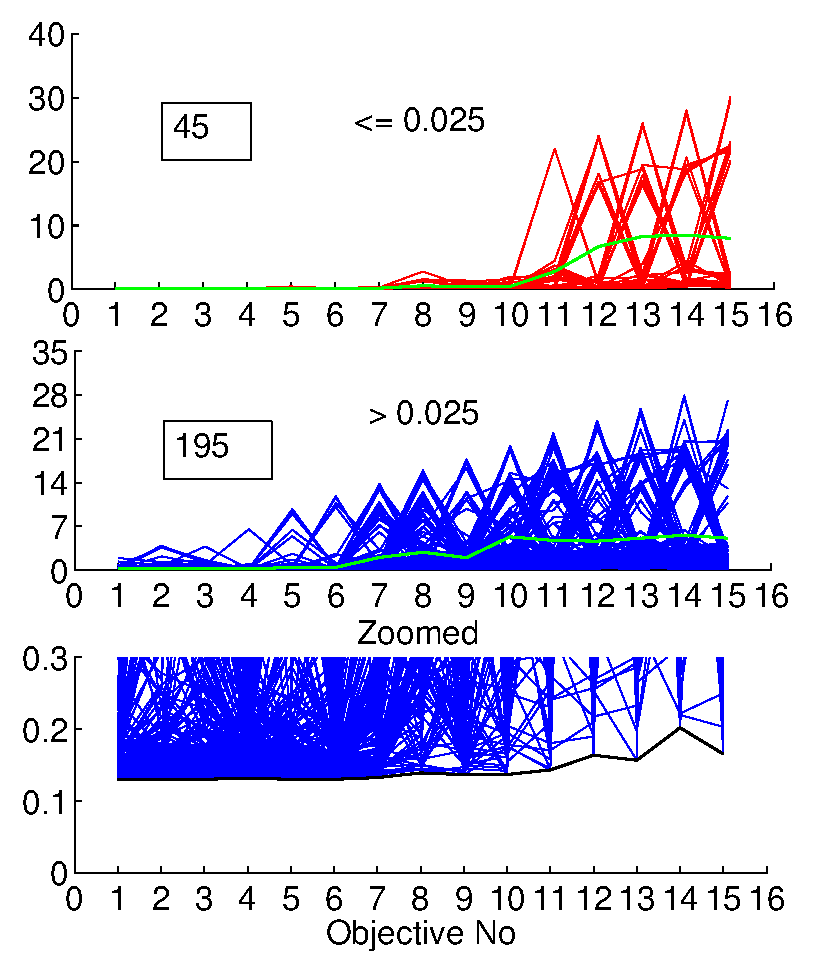
\includegraphics[width=0.175\textwidth]{figures/experiments/wfg/nsgaiiiwfg9_15.eps}
	}	
%	\hspace{0em}
%	\subfigure[MOEA/D]
%	{
%		\label{fig:moead9_15}
%		\includegraphics[width=0.175\textwidth]{figures/experiments/wfg/moeadwfg9_15.eps}
%	}
	\hspace{0em}
	\subfigure[FD-NSGAII]
	{
		\label{fig:zhenan9_15}
		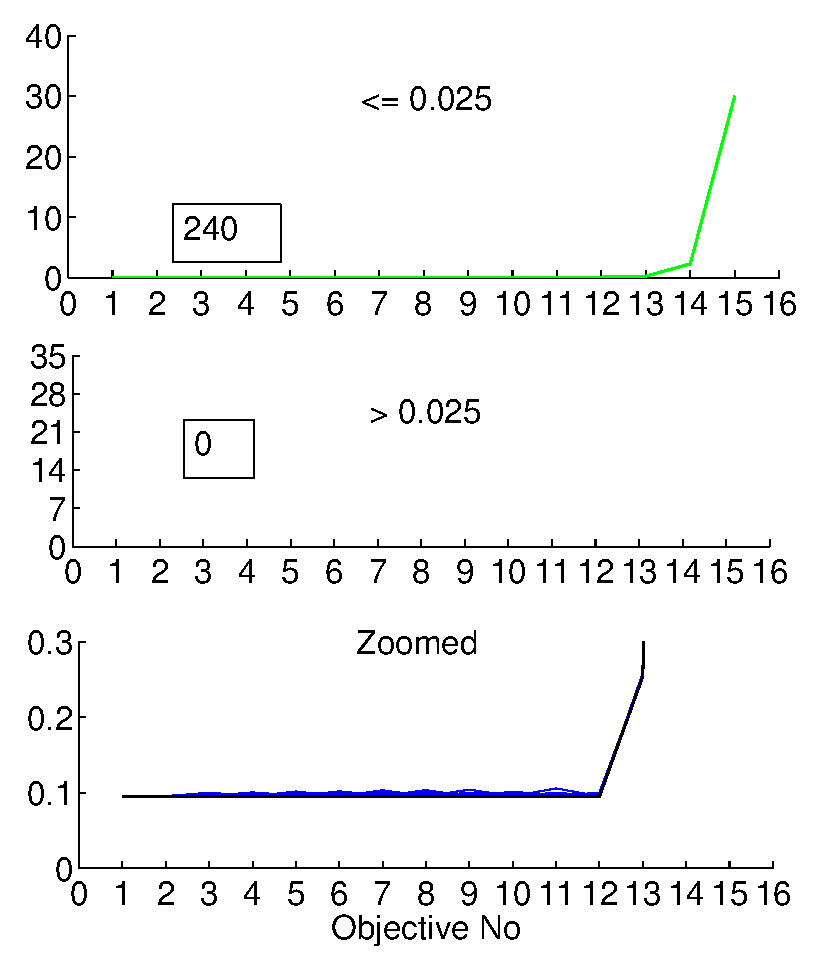
\includegraphics[width=0.175\textwidth]{figures/experiments/wfg/zhenanwfg9_15.eps}
	}
%	\hspace{0em}	
%	\subfigure[HypE]
%	{
%		\label{fig:hype9_15}
%		\includegraphics[width=0.175\textwidth]{figures/experiments/wfg/hypewfg9_15.eps}
%	}
	\hspace{0em}
	\subfigure[SDE]
	{
		\label{fig:sde9_15}
		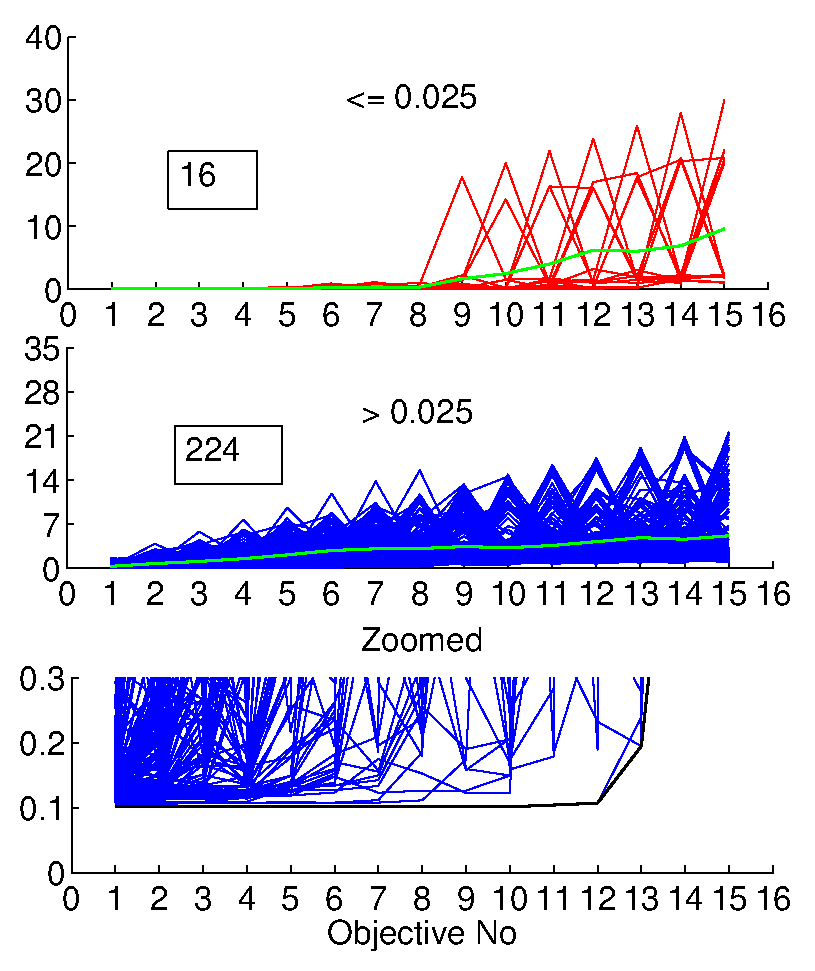
\includegraphics[width=0.175\textwidth]{figures/experiments/wfg/sdewfg9_15.eps}
	}
	\hspace{0em}
	\subfigure[PICEAg]
	{
		\label{fig:piceag9_15}
		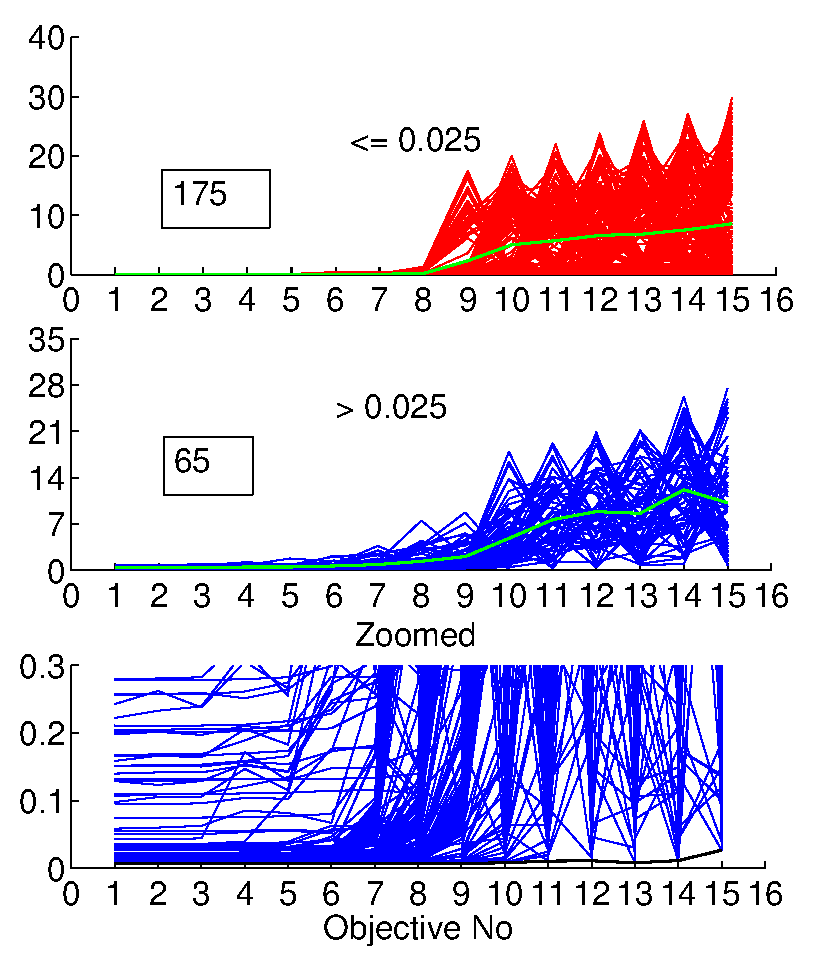
\includegraphics[width=0.175\textwidth]{figures/experiments/wfg/piceagwfg9_15.eps}
	}
	
\caption{Parallel coordinate plot of different algorithms for the WFG9 problem
with 15-objective. Here the non-dominated solutions are separated into two categories based on a threshold distance value from the normalized Pareto front. The solutions with a distance less than or equal to 0.025 is regarded as converged solutions (top figure, red colored), while the other ones are  regarded as non-converged solutions (middle figure, blue colored). Also, to observe the simultaneous minimization of different objectives, the bottom figure shows closer inspection of all the solutions.}
\label{fig:WFG9_15D}
\end{figure*}



\subsection{Experiments on DTLZ Problems}
We apply $F$-DEA and other competing algorithms on three DTLZ problems, DTLZ1, DTLZ3 and DTLZ7. These problems are complex compared to other DTLZ problems.  DTLZ1 is difficult to converge, DTLZ3 has a large number of local fronts and DTLZ7 is a disconnected problem. 
We use HV and IGD for comparison. But as DTLZ7 is a disconnected problem, it is difficult to get the reliable estimation of IGD value for this case. Hence, we did not employ IGD  for DTLZ7.  %The experimental results are presented as supplementary material, which show that the proposed $F$-DEA is able to outperform other competing algorithms in DTLZ1 and DTLZ7 in higher number of objectives~(Tables I-IV of supplementary material). For the remaining problems $F$-DEA showed competitive performance. The parallel coordinate plots~(Fig. 3 of supplementary material), also presented as supplementary material, show that the proposed algorithm is able to optimize each objective within limit successfully.

%\subsection{Experiment on DTLZ Problems}
%We apply $F$-DEA and other competing algorithms on three DTLZ problems, DTLZ1, DTLZ3 and DTLZ7. %These problems have been used in many previous studies and are different from the WFG ones in the sense that they have an identical range of values for each objective. 
%Hypervolume is used as before to compare
%the performances of different algorithms on the three DTLZ problems. We also employ here IGD values for comparing the performances of
%different algorithms on  DTLZ1 and DTLZ3 problems. As DTLZ7 is a disconnected problem, it is difficult to get reliable estimation of IGD value for this case. Hence, we did not employ IGD  for DTLZ7. 

Tables~\ref{table:dtlzhv} and ~\ref{table:dtlzIGD} show the performances of different algorithms on DTLZ1, DTLZ3 and DTLZ7 problems in terms of HV and IGD, respectively. %DTLZ7 is a disconnected problem, it is difficult to get reliable estimation of IGD value for this case. Hence, we did not employ IGD  for DTLZ7. 

%Tables~\ref{table:dtlzhvsummary} and ~\ref{table:dtlzigdsummary}, respectively, show the number of times $F$-DEA is found better, worse or equal than any competing algorithm based on the Wilcoxon rank-sum test applied on the HV and IGD values of the DTLZ problems. 
%
%Fig.~\ref{fig:dtlz710figure} shows the parallel coordinate plot of the competing algorithms for the DTLZ7 problem with 10-objective.

%The performances of different algorithms on each DTLZ problem is discussed as follows. 

\subsubsection{DTLZ1 Problem}

Although DTLZ1 has a simple linear Pareto Front $(\sum_{i=1}^{m} f_i=0.5)$, a large number of local optima~(= $11^5-1$)   
makes it difficult for an algorithm to converge into the hyper-plane. In terms of average HV and IGD,
NSGAIII was better than all other competing algorithms for a smaller number of objectives.
%$F$-DEA, MOEA/D, PICEAg, SDE were able to solve this problem with competitive performance.  
$F$-DEA, however, outperformed others as the number of objectives increased.
%For example, in terms of HV, $F$-DEA was found better than all competing algorithms from 10-objective to 25-objective. In terms of IGD, it beat all others in 7-, 10-, 15- and 20-objective and secured the second position after SDE in 12- and 25-objective.


%\subsubsection{DTLZ2 Problem}
%This is relatively an easy  problem with concave geometrical shape $(\sum_{i=1}^{m} f^2_i=1)$.
%%All of the competing algorithms were able to solve it.
%In terms of IGD, NSGAIII was the top performer from $2$-objective to $7$-objective.  
%SDE secured the top position based on HV for all but 2-objective.
%It also secured the top position in terms of IGD obtained for $10$-objective to $25$-objective. 
%The performances of $F$-DEA were close to the top performers both with respect to IGD and HV.  
%In terms of IGD for the $10$-objective to $25$-objective, the proposed algorithm
%secured the second position after SDE.

\subsubsection{DTLZ3 Problem}
%This problem has the same shape as DTLZ2 but it has a large number of local Pareto fronts parallel to the global one.

This problem has concave geometrical shape $(\sum_{i=1}^{m} f^2_i=1)$ with a large number of local Pareto fronts parallel to the global one. This property makes it a very challenging problem. SDE and MOEA/D were top performers on this problem. %Not all but $F$-DEA, SDE, MOEA/D, and PICEAg were able to solve this problem for a larger number of objectives, which could be seen by their non-zero HV values. 
In terms of HV and IGD, $F$-DEA was one of  the best performers in 3-objective 
and secured the second position after SDE for the 25-objective. 
It shared the second position with MOEA/D in many cases while compared with respect to HV and for a larger number of objectives.  
MOEA/D, however, outperformed $F$-DEA in terms of IGD values, which caused $F$-DEA to achieve overall the third position.


%\subsubsection{DTLZ4 Problem}
%Although DTLZ4 has same geometrical shape as DTLZ2 and DTLZ3, it challenges the ability of an algorithm to maintain diversity in the objective space by introducing variable density of solutions along the Pareto front. 
%The IGD values showed that $F$-DEA secured the first position
%in the 20-objective and the second position in rest of the objectives. 
%NSGAIII showed the best performance for a smaller number of 
%objectives and SDE for a larger ones. In terms of HV, $F$-DEA secured the third position after
%SDE and NSGAIII. %From the large values of IGD and small ones of HV, it is clear that both FD-NSGAII and HypE failed to maintain diversity.

\subsubsection{DTLZ7 Problem}
This problem has disconnected regions which make it interesting and challenging. In terms of HV, 
$F$-DEA exhibited superior performance for a larger number of objectives while SDE showed superior performance for a smaller ones~(Table~\ref{table:dtlzhv}). For example, 
SDE and MOEA/D jointly secured the first position  for 2-objective and the former one independently secured the first position from the 3-objective to 7-objective. NSGAIII obtained the second position for 3-objective 
and $F$-DEA secured the second position for  5-objective 
and 7-objective. For a larger number of objectives (from 10-objective to 25-objective), 
$F$-DEA was the best and PICEAg was next to it.
Most of the algorithms did not able to converge within the reference point bound  which constituted their small HV values for a larger
number of objectives.


Tables~\ref{table:dtlzhvsummary} and ~\ref{table:dtlzigdsummary}, respectively, show the number of times $F$-DEA is found better, worse or equal than any competing algorithm based on the Wilcoxon rank-sum test applied on the HV and IGD values of the DTLZ problems. 
In terms of HV and IGD, the three algorithms SDE, NSGAIII, PICEAg and $F$-DEA showed a very similar performance  for a smaller number of objectives, 2-objective to 7-objective. However, for higher number of objectives $F$-DEA outperforms others in DTLZ1, DTLZ7 problems and shows competitive performance with SDE and MOEA/D at DTLZ3 problem. %These observations were almost true when we compared $F$-DEA with others in terms of both HV and IGD.

%Fig.~\ref{fig:dtlz710figure} shows the parallel coordinate plot of the competing algorithms for the DTLZ7 problem with 10-objective. The upper bound of the last objective for this problem is $2\times m$ or $f_{10}\le 20$. It can be seen from the figure that $F$-DEA  was able to maintain diversity and convergence together within the Pareto optimal front. SDE~(Fig.~\ref{fig:dtlz710sdefigure}) and HypE~(Fig.~\ref{fig:dtlz710hypefigure}) exhibited similar convergence performance  but  $F$-DEA outperformed both of them in terms of diversity. PICEAg~(Fig.~\ref{fig:dtlz710piceagfigure}) converged in the first nine objective but few solutions converge on $10$th objective.

Fig.~\ref{fig:dtlz710figure} shows the parallel coordinate plot of the competing algorithms for the DTLZ7 problem with 10-objective.
The upper bound of the last objective for this problem is $2\times m$ or $f_{10}\le 20$. 
It can be seen from the figure that $F$-DEA  was able to maintain diversity and convergence together within the Pareto optimal front. SDE~(Fig.~\ref{fig:dtlz710sdefigure}) maintained diversity and convergence well but $F$-DEA outperforms SDE by having more objective value variation in the first 9 objectives. 
PICEAg~(Fig.~\ref{fig:dtlz710piceagfigure}) converged in the first nine objective but few solutions converge on $10$-th objective. Similarly, NSGAIII~(Fig.~\ref{fig:dtlz710nsgaiiifigure}) also converges in the first $9$ objectives but only few converges in the $10$-th objective.
FD-NSGAII~(Fig.~\ref{fig:dtlz710zhenanfigure}) converged solutions into a region as expected.



%
%It is clear from this table that in most of the cases $F$-DEA exhibits better performance on the DTLZ problems with a higher number of objectives. For example, $F$-DEA outperformed all other algorithms for the DTLZ2 problem with 10-objective to 20-objective. It also exhibited better performance on the disconnected problem DTLZ7 with 5-objective to 20-objective. Diversity maintenance is very much crucial for solving disconnected problem. The performance of our algorithm on the 
%DTLZ7 problem indicates the algorithm's better diversity maintenance ability. 
%In terms of average rank, $F$-DEA outperformed all other algorithms on the DTLZ1, DTLZ2, and DTLZ7, but it showed inferior performance compared to  MOEA/D and NSGAIII  for the DTLZ3 and DTLZ4 problems, respectively.   

\begin{figure*}[htbp] 
\centering 
 
	\subfigure[\textit{F}-DEA]
	{
		\label{fig:dtlz710fdeafigure}
		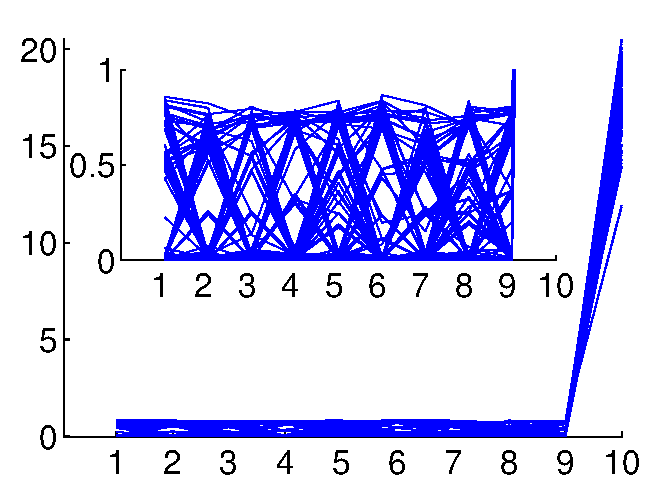
\includegraphics[width=0.170\textwidth]{figures/experiments/dtlz/fdeadtlz7_10.eps}
	}
	\hspace{0em}	
	\subfigure[NSGAIII]
	{
		\label{fig:dtlz710nsgaiiifigure}
		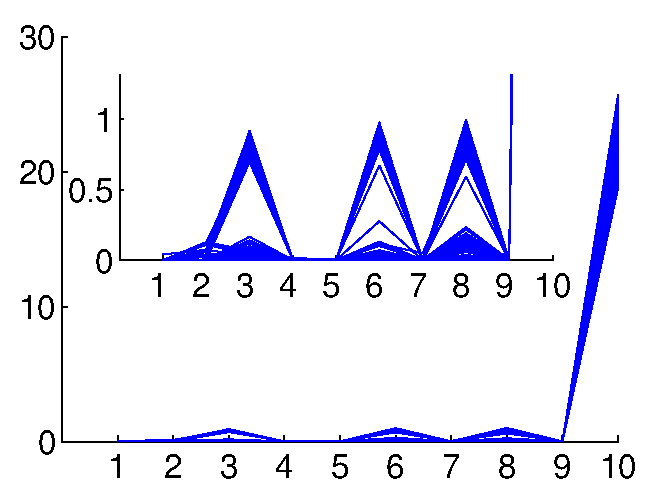
\includegraphics[width=0.170\textwidth]{figures/experiments/dtlz/nsgaiiidtlz7_10.eps}
	}	
	\hspace{0em}
%	\subfigure[MOEA/D]
%	{
%		\label{fig:dtlz710moeadfigure}
%		\includegraphics[width=0.170\textwidth]{figures/experiments/dtlz/moeaddtlz7_10.eps}
%	}	
	\hspace{0em}	
	\subfigure[FD-NSGAII]
	{
		\label{fig:dtlz710zhenanfigure}
		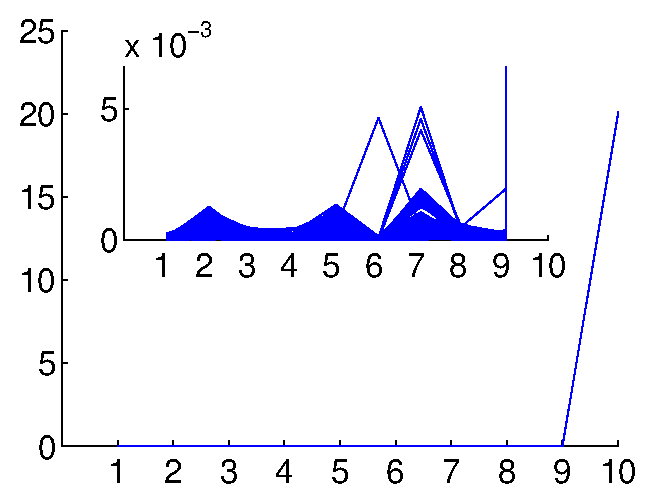
\includegraphics[width=0.170\textwidth]{figures/experiments/dtlz/zhenandtlz7_10.eps}
	}	
%	\hspace{0em}
%	\subfigure[HypE]
%	{
%		\label{fig:dtlz710hypefigure}
%		\includegraphics[width=0.170\textwidth]{figures/experiments/dtlz/hypedtlz7_10.eps}
%	}	
	\hspace{0em}	
	\subfigure[SDE]
	{
		\label{fig:dtlz710sdefigure}
		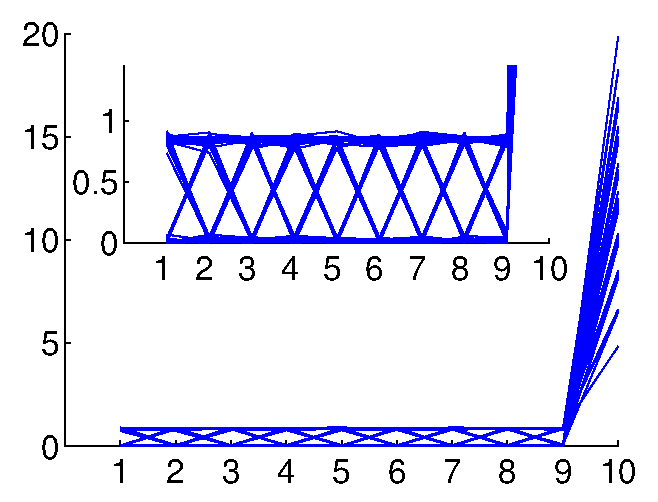
\includegraphics[width=0.170\textwidth]{figures/experiments/dtlz/sdedtlz7_10.eps}
	}	
	\hspace{0em}
	\subfigure[PICEAg]
	{
		\label{fig:dtlz710piceagfigure}
		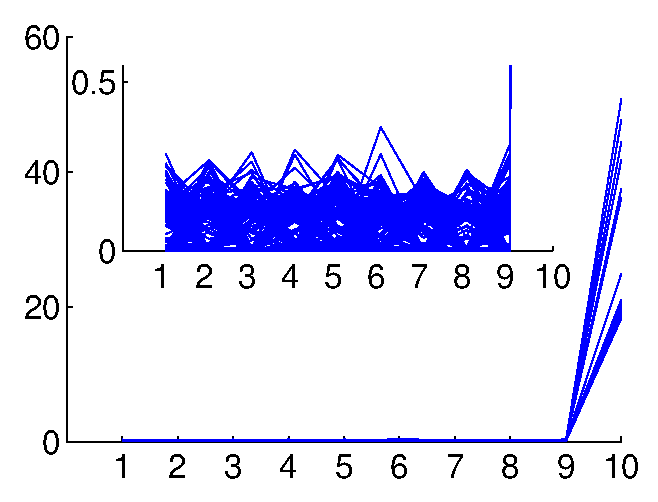
\includegraphics[width=0.170\textwidth]{figures/experiments/dtlz/piceagdtlz7_10.eps}
	}	
\caption{Parallel coordinate plot of all competing algorithms in $10-$ objective DTLZ7 problem. The inset figure shows the closer inspection of the first 9 objectives.}
\label{fig:dtlz710figure}
\end{figure*}
\begin{table*}[htbp]
\centering

\caption{Average HV of different algorithms on DTLZ1, DTLZ3 and DTLZ7 problems over 20 independent runs. The best result based on the Wilcoxon rank sum test with a significance level of $0.05$ is marked in bold-face. The rank of a particular algorithm is shown in bracket.}

\label{table:dtlzhv}

%\setlength{\tabcolsep}{2pt}
\renewcommand{\arraystretch}{1.1}
\begin{adjustbox}{width=1.0\textwidth,center}
%\resizebox{\textwidth}{!}{
\begin{tabular}{ccccccccc}
\thickhline
Prob. & \textit{m} & HYPE               & MOEA/D                       & FD-NSGAII          & SDE                          & NSGAIII                     & PICEA-g                     & F-DEA                       \\\thickhline
dtlz1 & 2          & 0.6596$\pm$0.0422(6)   & \textbf{0.7069$\pm$0.0005(2)}   & 0.0000$\pm$0.0000(7)   & \textbf{0.7066$\pm$0.0002(2)}    & \textbf{0.7063$\pm$0.0012(2)}   & 0.7061$\pm$0.0005(4.5)          & 0.7063$\pm$0.0002(4.5)          \\
      & 3          & 0.6849$\pm$0.5932(6)   & 1.0884$\pm$0.0088(5)            & 0.0000$\pm$0.0000(7)   & 1.1261$\pm$0.0023(3.5)           & \textbf{1.1246$\pm$0.0277(1.5)} & \textbf{1.1313$\pm$0.0045(1.5)} & 1.1249$\pm$0.0020(3.5)          \\
      & 5          & 0.0067$\pm$0.0116(6)   & 1.5142$\pm$0.0098(5)            & 0.0000$\pm$0.0000(7)   & 1.5481$\pm$0.0046(4)             & \textbf{1.5707$\pm$0.0076(1)}   & 1.5297$\pm$0.0459(2.5)          & 1.5582$\pm$0.0030(2.5)          \\
      & 7          & 0.6145$\pm$0.7117(6)   & 1.8803$\pm$0.0094(4)            & 0.0000$\pm$0.0000(7)   & 1.9108$\pm$0.0031(3)             & \textbf{1.9095$\pm$0.1091(1)}   & 1.7799$\pm$0.0819(5)            & 1.9272$\pm$0.0026(2)            \\
      & 10         & 0.6077$\pm$1.0526(6)   & 2.4924$\pm$0.0229(3)            & 0.0090$\pm$0.0331(7)   & 2.5591$\pm$0.0044(2)             & 1.7479$\pm$0.9172(4.5)          & 2.2692$\pm$0.3215(4.5)          & \textbf{2.5829$\pm$0.0024(1)}   \\
      & 12         & 0.0141$\pm$0.0231(6)   & 2.9727$\pm$0.0335(3)            & 0.0306$\pm$0.1175(7)   & 3.0855$\pm$0.0093(2)             & 1.8917$\pm$1.1930(4.5)          & 2.5134$\pm$0.6594(4.5)          & \textbf{3.1253$\pm$0.0034(1)}   \\
      & 15         & 0.7807$\pm$0.6792(6)   & 4.0354$\pm$0.0273(3)            & 0.0152$\pm$0.0680(7)   & 4.1336$\pm$0.0064(2)             & 3.8412$\pm$0.3188(4.5)          & 3.4812$\pm$1.0382(4.5)          & \textbf{4.1680$\pm$0.0021(1)}   \\
      & 20         & 0.0000$\pm$0.0000(6.5) & 6.4428$\pm$0.0967(3)            & 0.1024$\pm$0.2214(6.5) & 6.6532$\pm$0.0101(2)             & 3.2618$\pm$2.7249(4.5)          & 5.1065$\pm$2.0933(4.5)          & \textbf{6.7005$\pm$0.0072(1)}   \\
      & 25         & 0.3519$\pm$0.6122(5.5) & 0.0000$\pm$0.0000(7)            & 0.2169$\pm$0.3563(5.5) & 10.7567$\pm$0.0128(2)            & 6.9000$\pm$4.0868(4)            & 10.3842$\pm$0.3817(3)           & \textbf{10.8130$\pm$0.0069(1)}  \\\thickhline
%dtlz2 & 2          & 0.3953$\pm$0.0042(6)   & 0.4223$\pm$0.0000(1)            & 0.1099$\pm$0.0000(7)   & 0.4222$\pm$0.0000(2.5)           & 0.4222$\pm$0.0001(2.5)          & 0.4210$\pm$0.0002(5)            & 0.4217$\pm$0.0001(4)            \\
%      & 3          & 0.6160$\pm$0.0487(6)   & 0.7172$\pm$0.0085(5)            & 0.1209$\pm$0.0000(7)   & \textbf{0.7646$\pm$0.0007(1)}    & 0.7638$\pm$0.0006(2)            & 0.7600$\pm$0.0007(3)            & 0.7569$\pm$0.0012(4)            \\
%      & 5          & 0.9862$\pm$0.0894(6)   & 1.1694$\pm$0.0120(5)            & 0.1463$\pm$0.0000(7)   & \textbf{1.3040$\pm$0.0028(1)}    & 1.2995$\pm$0.0007(2)            & 1.2975$\pm$0.0021(3)            & 1.2847$\pm$0.0026(4)            \\
%      & 7          & 1.1859$\pm$0.0833(6)   & 1.6068$\pm$0.0124(5)            & 0.1770$\pm$0.0000(7)   & \textbf{1.7729$\pm$0.0024(1)}    & 1.7193$\pm$0.1551(3)            & 1.7582$\pm$0.0069(2)            & 1.7469$\pm$0.0045(4)            \\
%      & 10         & 1.5584$\pm$0.0502(6)   & 2.3023$\pm$0.0203(4)            & 0.2357$\pm$0.0000(7)   & \textbf{2.5098$\pm$0.0017(1)}    & 1.8555$\pm$0.2055(5)            & 2.4646$\pm$0.0380(2.5)          & 2.4854$\pm$0.0059(2.5)          \\
%      & 12         & 1.5474$\pm$0.1067(6)   & 2.6923$\pm$0.0658(3.5)          & 0.2852$\pm$0.0000(7)   & \textbf{3.0618$\pm$0.0032(1)}    & 2.1792$\pm$0.2725(5)            & 2.7169$\pm$0.1602(3.5)          & 3.0037$\pm$0.0180(2)            \\
%      & 15         & 2.0251$\pm$0.2760(6)   & 3.7780$\pm$0.0643(4)            & 0.3796$\pm$0.0000(7)   & \textbf{4.1362$\pm$0.0030(1)}    & 3.1109$\pm$0.2047(5)            & 3.8769$\pm$0.1392(3)            & 4.1171$\pm$0.0083(2)            \\
%      & 20         & 2.7181$\pm$0.9549(6)   & 5.9789$\pm$0.1165(3.5)          & 0.6114$\pm$0.0000(7)   & \textbf{6.7068$\pm$0.0018(1)}    & 5.2380$\pm$0.5474(5)            & 5.9443$\pm$0.2673(3.5)          & 6.6499$\pm$0.0300(2)            \\
%      & 25         & 5.8982$\pm$0.5908(6)   & 9.6726$\pm$0.0691(4)            & 0.9846$\pm$0.0001(7)   & \textbf{10.8225$\pm$0.0023(1)}   & 8.9515$\pm$0.9008(5)            & 10.4096$\pm$0.3050(3)           & 10.8131$\pm$0.0059(2)           \\\thickhline
dtlz3 & 2          & 0.0830$\pm$0.1437(5.5) & 0.4139$\pm$0.0068(1.5)          & 0.0000$\pm$0.0000(7)   & \textbf{0.4104$\pm$0.0096(1.5)}  & 0.3796$\pm$0.0911(4)            & 0.1540$\pm$0.1810(5.5)          & 0.4041$\pm$0.0120(3)            \\
      & 3          & 0.1338$\pm$0.2317(5.5) & 0.6931$\pm$0.0150(3)            & 0.0000$\pm$0.0000(7)   & 0.4101$\pm$0.2904(4)             & 0.1595$\pm$0.2052(5.5)          & \textbf{0.4626$\pm$0.3281(1.5)} & \textbf{0.7261$\pm$0.0130(1.5)} \\
      & 5          & 0.0000$\pm$0.0000(6.5) & 1.1638$\pm$0.0221(2)            & 0.0000$\pm$0.0000(6.5) & \textbf{1.2779$\pm$0.0197(1)}    & 0.0673$\pm$0.1730(4.5)          & 0.6202$\pm$0.4698(3)            & 0.1174$\pm$0.2130(4.5)          \\
      & 7          & 0.0000$\pm$0.0000(6)   & 1.4667$\pm$0.3553(2)            & 0.0000$\pm$0.0000(6)   & \textbf{1.7475$\pm$0.0093(1)}    & 0.1311$\pm$0.3230(6)            & 0.5283$\pm$0.6051(3.5)          & 0.8720$\pm$0.7061(3.5)          \\
      & 10         & 0.0000$\pm$0.0000(6)   & 1.9846$\pm$0.4769(2.5)          & 0.0000$\pm$0.0000(6)   & \textbf{2.4098$\pm$0.2289(1)}    & 0.0000$\pm$0.0000(6)            & 0.6794$\pm$0.7619(4)            & 1.7546$\pm$0.9708(2.5)          \\
      & 12         & 0.0000$\pm$0.0000(5.5) & 1.6366$\pm$1.0472(2.5)          & 0.0000$\pm$0.0000(5.5) & \textbf{2.5020$\pm$1.0833(1)}    & 0.0000$\pm$0.0000(5.5)          & 0.1847$\pm$0.5736(5.5)          & 1.3304$\pm$1.3433(2.5)          \\
      & 15         & 0.0000$\pm$0.0000(6)   & 3.4835$\pm$0.0759(2.5)          & 0.0000$\pm$0.0000(6)   & \textbf{4.0894$\pm$0.0245(1)}    & 0.0000$\pm$0.0000(6)            & 0.9834$\pm$1.3996(4)            & 2.2773$\pm$1.8582(2.5)          \\
      & 20         & 0.0000$\pm$0.0000(6)   & 4.6077$\pm$1.7082(2)            & 0.0000$\pm$0.0000(6)   & \textbf{6.5836$\pm$0.0571(1)}    & 0.0000$\pm$0.0000(6)            & 1.3989$\pm$2.1580(3.5)          & 1.5242$\pm$2.5204(3.5)          \\
      & 25         & 0.0000$\pm$0.0000(5.5) & 0.0000$\pm$0.0000(5.5)          & 0.0000$\pm$0.0000(5.5) & \textbf{10.7668$\pm$0.0279(1)}   & 0.0000$\pm$0.0000(5.5)          & 5.5089$\pm$3.6702(2.5)          & 3.9419$\pm$4.2086(2.5)          \\\thickhline
%dtlz4 & 2          & 0.2107$\pm$0.1745(6)   & 0.3911$\pm$0.0961(1)            & 0.1099$\pm$0.0000(7)   & 0.4222$\pm$0.0000(3)             & 0.4223$\pm$0.0000(2)            & 0.4212$\pm$0.0001(5)            & 0.4217$\pm$0.0001(4)            \\
%      & 3          & 0.5398$\pm$0.1510(6)   & 0.6848$\pm$0.0957(5)            & 0.1209$\pm$0.0000(7)   & 0.7501$\pm$0.0672(1)             & 0.7219$\pm$0.1024(2)            & 0.7591$\pm$0.0007(3)            & 0.7573$\pm$0.0009(4)            \\
%      & 5          & 0.9247$\pm$0.1222(6)   & 1.1728$\pm$0.0561(5)            & 0.1463$\pm$0.0000(7)   & \textbf{1.3001$\pm$0.0329(1)}    & 1.3031$\pm$0.0010(2)            & 1.2928$\pm$0.0035(3)            & 1.2889$\pm$0.0019(4)            \\
%      & 7          & 1.0358$\pm$0.3297(6)   & 1.6415$\pm$0.0852(5)            & 0.1770$\pm$0.0000(7)   & 1.7707$\pm$0.0036(1)             & 1.7616$\pm$0.0051(2)            & 1.7483$\pm$0.0167(3.5)          & 1.7540$\pm$0.0025(3.5)          \\
%      & 10         & 1.2239$\pm$0.0970(6)   & 2.4014$\pm$0.0554(5)            & 0.2356$\pm$0.0000(7)   & \textbf{2.5058$\pm$0.0029(1)}    & 2.4908$\pm$0.0366(2)            & 2.4802$\pm$0.0111(4)            & 2.4951$\pm$0.0023(3)            \\
%      & 12         & 0.5542$\pm$0.5997(6)   & 2.8696$\pm$0.0733(5)            & 0.2850$\pm$0.0001(7)   & \textbf{3.0586$\pm$0.0060(1)}    & 2.9287$\pm$0.1026(4)            & 2.9963$\pm$0.0209(3)            & 3.0480$\pm$0.0044(2)            \\
%      & 15         & 0.9156$\pm$0.3491(6)   & 4.0652$\pm$0.0213(4.5)          & 0.3793$\pm$0.0002(7)   & \textbf{4.1406$\pm$0.0020(1.5)}  & 4.0400$\pm$0.1085(4.5)          & 4.1160$\pm$0.0078(3)            & \textbf{4.1402$\pm$0.0019(1.5)} \\
%      & 20         & 0.5678$\pm$0.2077(7)   & 6.6212$\pm$0.0255(5)            & 0.6630$\pm$0.1608(6)   & \textbf{6.7076$\pm$0.0020(1)}    & 6.6739$\pm$0.0408(3.5)          & 6.6902$\pm$0.0047(3.5)          & 6.7038$\pm$0.0034(2)            \\
%      & 25         & 1.1185$\pm$0.7458(6.5) & 10.7742$\pm$0.0087(5)           & 1.1514$\pm$0.3481(6.5) & \textbf{10.8284$\pm$0.0006(1.5)} & 10.8250$\pm$0.0153(1.5)         & 10.8247$\pm$0.0013(4)           & 10.8277$\pm$0.0013(3)           \\\thickhline
dtlz7 & 2          & 0.3190$\pm$0.0101(6)   & \textbf{0.3337$\pm$0.0000(1.5)} & 0.1133$\pm$0.0143(7)   & \textbf{0.3337$\pm$0.0000(1.5)}  & 0.3337$\pm$0.0000(3)            & 0.3165$\pm$0.0372(5)            & 0.3334$\pm$0.0001(4)            \\
      & 3          & 0.3753$\pm$0.0141(6)   & 0.4103$\pm$0.0070(5)            & 0.1207$\pm$0.0001(7)   & \textbf{0.4351$\pm$0.0008(1)}    & 0.4327$\pm$0.0006(2)            & 0.4033$\pm$0.0560(3.5)          & 0.4281$\pm$0.0015(3.5)          \\
      & 5          & 0.4074$\pm$0.0018(5)   & 0.3423$\pm$0.0376(6)            & 0.1436$\pm$0.0003(7)   & \textbf{0.5248$\pm$0.0036(1)}    & 0.4318$\pm$0.0241(3.5)          & 0.4079$\pm$0.0494(3.5)          & 0.4834$\pm$0.0038(2)            \\
      & 7          & 0.3774$\pm$0.0159(3)   & 0.2361$\pm$0.0553(6)            & 0.1535$\pm$0.0030(7)   & \textbf{0.5093$\pm$0.0074(1)}    & 0.3231$\pm$0.0322(5)            & 0.3547$\pm$0.0204(4)            & 0.4822$\pm$0.0061(2)            \\
      & 10         & 0.2845$\pm$0.0445(3.5) & 0.0345$\pm$0.0243(7)            & 0.1649$\pm$0.0014(5)   & 0.3119$\pm$0.0479(3.5)           & 0.0848$\pm$0.0555(6)            & 0.3405$\pm$0.0253(2)            & \textbf{0.4563$\pm$0.0149(1)}   \\
      & 12         & 0.2441$\pm$0.0042(2.5) & 0.0052$\pm$0.0063(6)            & 0.1735$\pm$0.0048(4.5) & 0.1591$\pm$0.0329(4.5)           & 0.0010$\pm$0.0023(7)            & 0.2522$\pm$0.0418(2.5)          & \textbf{0.5079$\pm$0.0507(1)}   \\
      & 15         & 0.2748$\pm$0.0394(3)   & 0.0002$\pm$0.0003(6)            & 0.1636$\pm$0.0012(4)   & 0.0283$\pm$0.0099(5)             & 0.0001$\pm$0.0005(7)            & 0.3346$\pm$0.0274(2)            & \textbf{0.3831$\pm$0.0245(1)}   \\
      & 20         & 0.1714$\pm$0.0362(2)   & 0.0000$\pm$0.0000(6.5)          & 0.0834$\pm$0.0066(3.5) & 0.0086$\pm$0.0125(5)             & 0.0000$\pm$0.0000(6.5)          & 0.0889$\pm$0.0836(3.5)          & \textbf{0.3275$\pm$0.0571(1)}   \\
      & 25         & 0.0000$\pm$0.0000(5.5) & 0.0000$\pm$0.0000(5.5)          & 0.0000$\pm$0.0000(5.5) & 0.0005$\pm$0.0005(3)             & 0.0000$\pm$0.0000(5.5)          & 0.1203$\pm$0.0984(2)            & \textbf{0.1932$\pm$0.0399(1)}  \\\thickhline
\end{tabular}
%}
\end{adjustbox}
\end{table*}
\begin{table*}[htbp]
\centering

\caption{Average IGD of different algorithms on DTLZ1 and DTLZ3 problems over 20 independent runs. The best result based on the Wilcoxon rank sum test with a significance level of $0.05$ is marked in bold-face. The rank of a particular algorithm is shown in bracket.}
\label{table:dtlzIGD}
%\setlength{\tabcolsep}{2pt}
\renewcommand{\arraystretch}{1.1}
\begin{adjustbox}{width=1.0\textwidth,center}
%\resizebox{\textwidth}{!}{
\begin{tabular}{lllllllll}
\thickhline
Prob. & \multicolumn{1}{c}{\textit{m}} & \multicolumn{1}{c}{HYPE} & \multicolumn{1}{c}{MOEA/D} & \multicolumn{1}{c}{FD-NSGAII} & \multicolumn{1}{c}{SDE}   & \multicolumn{1}{c}{NSGAIII}                   & \multicolumn{1}{c}{PICEA-g}          & \multicolumn{1}{c}{F-DEA} \\\thickhline
dtlz1 & 2                              & 0.0016$\pm$0.0010(6)         & 0.0000$\pm$0.0000(2)          & 0.3873$\pm$0.1489(7)              & 0.0000$\pm$0.0000(3)          & \textbf{0.0000$\pm$0.0000(1)}                     & 0.0000$\pm$0.0000(4)                     & 0.0001$\pm$0.0000(5)          \\
      & 3                              & 0.0117$\pm$0.0164(6)         & 0.0021$\pm$0.0001(5)          & 0.5881$\pm$0.2721(7)              & \textbf{0.0011$\pm$0.0000(1)} & 0.0009$\pm$0.0011(4)                              & 0.0011$\pm$0.0002(2)                     & 0.0012$\pm$0.0001(3)          \\
      & 5                              & 0.0512$\pm$0.0312(6)         & 0.0052$\pm$0.0000(4)          & 0.3606$\pm$0.1076(7)              & 0.0041$\pm$0.0000(2)          & \multicolumn{1}{r}{\textbf{0.0020$\pm$0.0013(1)}} & 0.0076$\pm$0.0033(5)                     & 0.0042$\pm$0.0001(3)          \\
      & 7                              & 0.0592$\pm$0.0444(6)         & 0.0077$\pm$0.0001(4)          & 0.2067$\pm$0.0495(7)              & 0.0067$\pm$0.0001(2.5)        & \multicolumn{1}{r}{0.0040$\pm$0.0044(2.5)}        & 0.0182$\pm$0.0020(5)                     & \textbf{0.0063$\pm$0.0001(1)} \\
      & 10                             & 0.0631$\pm$0.0359(6)         & 0.0116$\pm$0.0007(3)          & 0.0821$\pm$0.0310(7)              & 0.0092$\pm$0.0001(2)          & 0.0254$\pm$0.0083(5)                              & 0.0226$\pm$0.0021(4)                     & \textbf{0.0083$\pm$0.0002(1)} \\
      & 12                             & 0.1058$\pm$0.0682(7)         & 0.0152$\pm$0.0007(3)          & 0.1077$\pm$0.0509(6)              & \textbf{0.0113$\pm$0.0002(1)} & 0.0335$\pm$0.0125(4)                              & 0.0301$\pm$0.0106(5)                     & 0.0116$\pm$0.0004(2)          \\
      & 15                             & 0.0929$\pm$0.0674(7)         & 0.0132$\pm$0.0010(3)          & 0.0775$\pm$0.0366(6)              & 0.0095$\pm$0.0002(2)          & 0.0202$\pm$0.0016(4)                              & 0.0235$\pm$0.0058(5)                     & \textbf{0.0094$\pm$0.0002(1)} \\
      & 20                             & 0.1201$\pm$0.0407(7)         & 0.0204$\pm$0.0006(3)          & 0.0728$\pm$0.0335(6)              & 0.0155$\pm$0.0003(2)          & 0.0370$\pm$0.0128(5)                              & 0.0320$\pm$0.0110(4)                     & \textbf{0.0141$\pm$0.0009(1)} \\
      & 25                             & 0.0165$\pm$0.0093(6)         & 0.1045$\pm$0.0217(7)          & 0.0150$\pm$0.0049(5)              & \textbf{0.0033$\pm$0.0000(1)} & 0.0077$\pm$0.0029(4)                              & 0.0060$\pm$0.0003(3)                     & 0.0036$\pm$0.0002(2)          \\\thickhline
%dtlz2 & 2                              & 0.0032$\pm$0.0017(6)         & 0.0001$\pm$0.0000(2)          & 0.0611$\pm$0.0000(7)              & 0.0006$\pm$0.0001(5)          & \textbf{0.0000$\pm$0.0000(1)}                     & 0.0002$\pm$0.0000(4)                     & 0.0002$\pm$0.0000(3)          \\
%      & 3                              & 0.0153$\pm$0.0024(6)         & 0.0054$\pm$0.0003(5)          & 0.0744$\pm$0.0000(7)              & 0.0046$\pm$0.0001(4)          & \textbf{0.0002$\pm$0.0001(1)}                     & 0.0028$\pm$0.0000(2)                     & 0.0031$\pm$0.0000(3)          \\
%      & 5                              & 0.0250$\pm$0.0016(6)         & 0.0152$\pm$0.0002(5)          & 0.0808$\pm$0.0000(7)              & 0.0127$\pm$0.0002(4)          & \textbf{0.0008$\pm$0.0001(1)}                     & 0.0111$\pm$0.0002(2)                     & 0.0115$\pm$0.0002(3)          \\
%      & 7                              & 0.0350$\pm$0.0042(6)         & 0.0230$\pm$0.0002(5)          & 0.0858$\pm$0.0000(7)              & 0.0165$\pm$0.0004(2)          & 0.0046$\pm$0.0132(3.5)                            & \textbf{0.0153$\pm$0.0010(1)}            & 0.0175$\pm$0.0005(3.5)        \\
%      & 10                             & 0.0501$\pm$0.0045(6)         & 0.0298$\pm$0.0004(4)          & 0.0876$\pm$0.0000(7)              & \textbf{0.0197$\pm$0.0005(1)} & 0.0583$\pm$0.0136(5)                              & 0.0241$\pm$0.0072(3)                     & 0.0223$\pm$0.0006(2)          \\
%      & 12                             & 0.0688$\pm$0.0056(6)         & 0.0399$\pm$0.0037(3)          & 0.1044$\pm$0.0000(7)              & \textbf{0.0242$\pm$0.0015(1)} & 0.0759$\pm$0.0166(5)                              & 0.0642$\pm$0.0088(4)                     & 0.0305$\pm$0.0016(2)          \\
%      & 15                             & 0.0622$\pm$0.0029(5)         & 0.0359$\pm$0.0030(3)          & 0.0854$\pm$0.0000(7)              & \textbf{0.0198$\pm$0.0013(1)} & 0.0668$\pm$0.0030(6)                              & 0.0534$\pm$0.0061(4)                     & 0.0250$\pm$0.0009(2)          \\
%      & 20                             & 0.0755$\pm$0.0024(6)         & 0.0528$\pm$0.0031(3)          & 0.0941$\pm$0.0000(7)              & \textbf{0.0202$\pm$0.0016(1)} & 0.0752$\pm$0.0074(5)                              & 0.0729$\pm$0.0037(4)                     & 0.0306$\pm$0.0035(2)          \\
%      & 25                             & 0.0197$\pm$0.0004(6)         & 0.0151$\pm$0.0003(3)          & 0.0239$\pm$0.0000(7)              & \textbf{0.0094$\pm$0.0000(1)} & 0.0191$\pm$0.0015(5)                              & 0.0170$\pm$0.0013(4)                     & 0.0102$\pm$0.0002(2)          \\\thickhline
dtlz3 & 2                              & 0.0435$\pm$0.0396(5)         & \textbf{0.0004$\pm$0.0003(1)} & 1.6814$\pm$0.7393(7)              & 0.0008$\pm$0.0003(2)          & 0.0039$\pm$0.0122(4)                              & 0.0586$\pm$0.0755(6)                     & 0.0008$\pm$0.0005(3)          \\
      & 3                              & 0.1586$\pm$0.1130(6)         & 0.0056$\pm$0.0004(2)          & 1.1440$\pm$0.4942(7)              & 0.0271$\pm$0.0269(3)          & 0.0493$\pm$0.0292(4)                              & 0.0317$\pm$0.0395(5)                     & \textbf{0.0037$\pm$0.0003(1)} \\
      & 5                              & 0.6058$\pm$0.2773(6)         & 0.0150$\pm$0.0004(2)          & 0.9245$\pm$0.2767(7)              & \textbf{0.0130$\pm$0.0005(1)} & 0.1037$\pm$0.0649(5)                              & 0.0608$\pm$0.0397(3)                     & 0.0904$\pm$0.0624(4)          \\
      & 7                              & 0.9081$\pm$0.3801(7)         & 0.0272$\pm$0.0120(2)          & 0.8025$\pm$0.2808(6)              & \textbf{0.0173$\pm$0.0006(1)} & 0.1592$\pm$0.1150(5)                              & 0.1012$\pm$0.0586(4)                     & 0.0528$\pm$0.0418(3)          \\
      & 10                             & 0.9161$\pm$0.2690(7)         & 0.0404$\pm$0.0119(2)          & 0.6995$\pm$0.2610(5)              & \textbf{0.0245$\pm$0.0048(1)} & 0.6902$\pm$0.3276(6)                              & 0.1096$\pm$0.0593(4)                     & 0.0396$\pm$0.0246(3)          \\
      & 12                             & 1.3816$\pm$0.4275(6)         & 0.0786$\pm$0.0540(2)          & 1.1271$\pm$0.4369(5)              & \textbf{0.0494$\pm$0.0359(1)} & 1.0651$\pm$0.6395(7)                              & 0.2625$\pm$0.1429(4)                     & 0.1004$\pm$0.0884(3)          \\
      & 15                             & 0.8515$\pm$0.3101(6)         & 0.0469$\pm$0.0046(2)          & 0.5108$\pm$0.1996(5)              & \textbf{0.0289$\pm$0.0031(1)} & 0.9245$\pm$0.4516(7)                              & 0.1055$\pm$0.0299(4)                     & 0.0510$\pm$0.0317(3)          \\
      & 20                             & 1.2758$\pm$0.4770(6)         & 0.0761$\pm$0.0293(2)          & 0.6600$\pm$0.2519(5)              & \textbf{0.0374$\pm$0.0033(1)} & 1.4316$\pm$0.4919(7)                              & 0.1644$\pm$0.0839(4)                     & 0.1337$\pm$0.0769(3)          \\
      & 25                             & 2.8646$\pm$0.7739(6)         & 3.0273$\pm$0.3555(7)          & 0.1204$\pm$0.0454(4)              & \textbf{0.0107$\pm$0.0010(1)} & 0.3112$\pm$0.0964(5)                              & 0.0249$\pm$0.0084(3)                     & 0.0230$\pm$0.0098(2)          \\\thickhline
%dtlz4 & 2                              & 0.0162$\pm$0.0266(6)         & 0.0062$\pm$0.0188(5)          & 0.0612$\pm$0.0000(7)              & 0.0006$\pm$0.0001(4)          & \textbf{0.0000$\pm$0.0000(1)}                     & 0.0002$\pm$0.0000(3)                     & 0.0002$\pm$0.0000(2)          \\
%      & 3                              & 0.0383$\pm$0.0204(6)         & 0.0118$\pm$0.0160(5)          & 0.0746$\pm$0.0000(7)              & 0.0068$\pm$0.0099(4)          & 0.0065$\pm$0.0158(3)                              & \textbf{0.0029$\pm$0.0000(1)}            & 0.0031$\pm$0.0000(2)          \\
%      & 5                              & 0.0475$\pm$0.0080(6)         & 0.0193$\pm$0.0087(5)          & 0.0809$\pm$0.0000(7)              & 0.0140$\pm$0.0050(4)          & \textbf{0.0010$\pm$0.0002(1)}                     & 0.0113$\pm$0.0002(3)                     & 0.0112$\pm$0.0002(2)          \\
%      & 7                              & 0.0561$\pm$0.0093(6)         & 0.0251$\pm$0.0077(5)          & 0.0858$\pm$0.0000(7)              & 0.0180$\pm$0.0004(3)          & \textbf{0.0019$\pm$0.0009(1)}                     & 0.0173$\pm$0.0033(4)                     & 0.0178$\pm$0.0003(2)          \\
%      & 10                             & 0.0579$\pm$0.0057(6)         & 0.0310$\pm$0.0046(5)          & 0.0876$\pm$0.0000(7)              & 0.0225$\pm$0.0007(3)          & \textbf{0.0036$\pm$0.0071(1)}                     & 0.0216$\pm$0.0028(4)                     & 0.0225$\pm$0.0005(2)          \\
%      & 12                             & 0.0808$\pm$0.0023(6)         & 0.0457$\pm$0.0069(5)          & 0.1044$\pm$0.0000(7)              & \textbf{0.0248$\pm$0.0025(1)} & 0.0328$\pm$0.0156(4)                              & 0.0368$\pm$0.0042(3)                     & 0.0269$\pm$0.0008(2)          \\
%      & 15                             & 0.0652$\pm$0.0026(6)         & 0.0327$\pm$0.0025(5)          & 0.0854$\pm$0.0000(7)              & \textbf{0.0203$\pm$0.0009(1)} & 0.0279$\pm$0.0109(4)                              & 0.0271$\pm$0.0021(3)                     & 0.0224$\pm$0.0005(2)          \\
%      & 20                             & 0.0804$\pm$0.0048(6)         & 0.0420$\pm$0.0021(5)          & 0.0938$\pm$0.0010(7)              & 0.0281$\pm$0.0013(2)          & 0.0299$\pm$0.0126(3)                              & \multicolumn{1}{c}{0.0327$\pm$0.0015(4)} & \textbf{0.0247$\pm$0.0019(1)} \\
%      & 25                             & 0.0203$\pm$0.0009(6)         & 0.0117$\pm$0.0001(5)          & 0.0237$\pm$0.0003(7)              & \textbf{0.0097$\pm$0.0000(1)} & 0.0100$\pm$0.0005(4)                              & \multicolumn{1}{c}{0.0104$\pm$0.0001(3)} & 0.0102$\pm$0.0001(2)   \\\thickhline      
\end{tabular}
%}
\end{adjustbox}
\end{table*}
\begin{table}[htbp]
\centering
\caption{Summary of HV performance of competing algorithms for DTLZ1, DTLZ3 and DTLZ7 problems. Here B, E AND W indicate the number of times  $F$-DEA was found better compared to a particular algorithm.}

\label{table:dtlzhvsummary}

%\setlength{\tabcolsep}{2pt}
\renewcommand{\arraystretch}{1.1}
\begin{adjustbox}{width=0.50\textwidth,center}
\begin{tabular}{c|cccccc}
\thickhline
DTLZ & \multicolumn{6}{c}{HV Performance on 2-  and 3- objective} \\\thickhline
F-DEA vs & HypE & MOEA/D & FD-NSGAII & SDE & NSGAIII & PICEA-g \\\thickhline
B & 6 & 3 & 6 & 1 & 2 & 2 \\
E & 0 & 0 & 0 & 1 & 0 & 3 \\
W & 0 & 3 & 0 & 4 & 4 & 1 \\\thickhline
 & \multicolumn{6}{c}{HV Performance on 5- and 7- objective} \\\thickhline
%F-DEA vs & HypE & MOEA/D & FD-NSGAII & SDE & NSGAIII & PICEA-g \\\thickhline
B & 6 & 4 & 6 & 2 & 3 & 3 \\
E & 0 & 0 & 0 & 0 & 1 & 2 \\
W & 0 & 2 & 0 & 4 & 2 & 1 \\\thickhline
 & \multicolumn{6}{c}{HV Performance on 10-, 12-, 15-, 20- and 25-objective} \\\thickhline
%F-DEA vs & HypE & MOEA/D & FD-NSGAII & SDE & NSGAIII & PICEA-g \\\thickhline
B & 15 & 11 & 15 & 10 & 15 & 13 \\
E & 0  & 3  & 0  & 0  & 0  & 2  \\
W & 0  & 1  & 0  & 5  & 0  & 0\\\thickhline
\end{tabular}
\end{adjustbox}
\end{table}

%
%\begin{table}[]
%\centering
%\caption{Summary of HV performance of competing algorithms for DTLZ1, DTLZ3 and DTLZ7 problems. Here B, E AND W indicate the number of times  $F$-DEA was found better compared to a particular algorithm.}
%
%\label{table:dtlzhvsummary}
%
%%\setlength{\tabcolsep}{2pt}
%\renewcommand{\arraystretch}{1.1}
%\begin{adjustbox}{width=0.45\textwidth,center}
%\begin{tabular}{c|cccccc}
%\thickhline
%DTLZ & \multicolumn{6}{c}{HV Performance on 2-  and 3- objective} \\\thickhline
%F-DEA vs & HypE & MOEA/D & FD-NSGAII & SDE & NSGAIII & PICEA-g \\\thickhline
%B & 10 & 5 & 10 & 1 & 2 & 4 \\
%E & 0 & 0 & 0 & 1 & 0 & 3 \\
%W & 0 & 5 & 0 & 8 & 8 & 3 \\\thickhline
% & \multicolumn{6}{c}{HV Performance on 5- and 7- objective} \\\thickhline
%%F-DEA vs & HypE & MOEA/D & FD-NSGAII & SDE & NSGAIII & PICEA-g \\\thickhline
%B & 10 & 8 & 10 & 2 & 3 & 3 \\
%E & 0 & 0 & 0 & 0 & 1 & 3 \\
%W & 0 & 2 & 0 & 8 & 6 & 4 \\\thickhline
% & \multicolumn{6}{c}{HV Performance on 10-, 12-, 15-, 20- and 25-objective} \\\thickhline
%%F-DEA vs & HypE & MOEA/D & FD-NSGAII & SDE & NSGAIII & PICEA-g \\\thickhline
%B & 25 & 21 & 25 & 10 & 23 & 22 \\
%E & 0 & 3 & 0 & 1 & 0 & 3 \\
%W & 0 & 1 & 0 & 14 & 2 & 0\\\thickhline
%\end{tabular}
%\end{adjustbox}
%\end{table}
\begin{table}[htbp]
\centering
\caption{Summary of IGD performance of competing algorithms for DTLZ1 and DTL3 problems. Here B, E AND W indicate the number of times  $F$-DEA was found better compared to a particular algorithm.}
\label{table:dtlzigdsummary}
%\setlength{\tabcolsep}{2pt}
\renewcommand{\arraystretch}{1.1}
\begin{adjustbox}{width=0.50\textwidth,center}
\begin{tabular}{c|cccccc}
\thickhline
DTLZ & \multicolumn{6}{c}{IGD Performance on 2-  and 3- objective} \\\thickhline
F-DEA vs & HypE & MOEA/D & FD-NSGAII & SDE & NSGAIII & PICEA-g \\\thickhline
B & 4 & 2 & 4 & 1 & 3 & 2 \\
E & 0 & 0 & 0 & 0 & 0 & 0 \\
W & 0 & 2 & 0 & 3 & 1 & 2 \\\thickhline
 & \multicolumn{6}{c}{IGD Performance on 5- and 7- objective} \\\thickhline
%F-DEA vs & HypE & MOEA/D & FD-NSGAII & SDE & NSGAIII & PICEA-g \\\thickhline
B & 4 & 2 & 4 & 1 & 3 & 3 \\
E & 0 & 0 & 0 & 0 & 0 & 0 \\
W & 0 & 2 & 0 & 3 & 1 & 1\\\thickhline
 & \multicolumn{6}{c}{IGD Performance on 10-, 12-, 15-, 20- and 25-objective} \\\thickhline
%F-DEA vs & HypE & MOEA/D & FD-NSGAII & SDE & NSGAIII & PICEA-g \\\thickhline
B & 10 & 6 & 10 & 3 & 10 & 10 \\
E & 0  & 0 & 0  & 0 & 0  & 0  \\
W & 0  & 4 & 0  & 7 & 0  & 0  \\\thickhline
\end{tabular}
\end{adjustbox}
\end{table}


%\begin{table}[]
%\centering
%\caption{Summary of IGD performance of competing algorithms for four DTLZ problems. Here B, E AND W indicate the number of times  $F$-DEA was found better compared to a particular algorithm.}
%\label{table:dtlzigdsummary}
%%\setlength{\tabcolsep}{2pt}
%\renewcommand{\arraystretch}{1.1}
%\begin{adjustbox}{width=0.45\textwidth,center}
%\begin{tabular}{c|cccccc}
%\thickhline
%DTLZ & \multicolumn{6}{c}{IGD Performance on 2-  and 3- objective} \\\thickhline
%F-DEA vs & HypE & MOEA/D & FD-NSGAII & SDE & NSGAIII & PICEA-g \\\thickhline
%B & 8 & 5 & 8 & 5 & 4 & 4 \\
%E & 0 & 0 & 0 & 0 & 0 & 0 \\
%W & 0 & 3 & 0 & 3 & 4 & 4 \\\thickhline
% & \multicolumn{6}{c}{IGD Performance on 5- and 7- objective} \\\thickhline
%%F-DEA vs & HypE & MOEA/D & FD-NSGAII & SDE & NSGAIII & PICEA-g \\\thickhline
%B & 8 & 6 & 8 & 4 & 3 & 5 \\
%E & 0 & 0 & 0 & 0 & 1 & 0 \\
%W & 0 & 2 & 0 & 4 & 4 & 3 \\\thickhline
% & \multicolumn{6}{c}{IGD Performance on 10-, 12-, 15-, 20- and 25-objective} \\\thickhline
%%F-DEA vs & HypE & MOEA/D & FD-NSGAII & SDE & NSGAIII & PICEA-g \\\thickhline
%B & 20 & 16 & 20 & 5 & 19 & 20 \\
%E & 0 & 0 & 0 & 0 & 0 & 0 \\
%W & 0 & 4 & 0 & 15 & 1 & 0 \\\thickhline
%\end{tabular}
%\end{adjustbox}
%\end{table}


%\subsection{Experiments on Rectangle Problems}
%All competing algorithms including $F$-DEA have been tested on three instances of degenerate Rectangle problem~\citep{rectangleproblem}. %The rectangle problem is a $4$-objective degenerate problem with two decision variables. 
%The three instances are with same 4-objective lines ($f_1=0, f_1=100, f_2=0$ and $f_2=100$) and their only difference is in the 2-variable search space (decision space) range. Following~\citep{rectangleproblem}, ranges are defined as $[x_1, x_2]\in [{-20}, 120]$, $[x_1, x_2]\in[{-10000}, 10000]$ and $[x_1, x_2]\in [{-10^{12}}, 10^{12}]$ for instance I, II and III respectively.
%The true Pareto front of this problem is a line in $4$-dimensional objective space. But the interesting properties of it are that the degenerate Pareto optimal solutions lie in a rectangle of the two-variable decision space and have similar images in the objective space.
%%The three instances were taken based on a small to a large ranges of the two decision variables. 
%During experiments, division parameter, $\lambda$, of NSGAIII's and $F$-DEA's were set $10$ and $60$, respectively. The number of weights used in MOEA/D was chosen as $28800$, while the number of goals for PICEAg was $400$. The population size was set to $288$.
%
%The visual plots presented in supplementary material~(Figs. 4, 5 and 6 of supplementary material) show that $F$-DEA is able to solve rectangle problems effectively. Specially, in case of a very large search space, $F$-DEA was able to outperform all competing algorithms. In the rectangle problem, any solution inside the parallel objectives' line can be only Pareto dominated by a solution in the same line whereas the solutions in corner are dominated by those reside in the broader region~\citep{rectangleproblem}. This property creates difficulty for Pareto
%based algorithm to converge. As the primary selection criterion of NSGAIII and PICEAg is based on Pareto, it makes problem for them reaching to the Pareto optimal front and
%solutions are distributed in crisscross~(Figs. 5 and 6 of supplementary material). Our F-DEA applied fuzzy-fitness criterion in its selection mechanism which alleviates the problem faced by Pareto dominance.

\subsection{Discussion}

The results presented in the previous sections and supplementary material give an idea about the performances of $F$-DEA with respect to different competing algorithms. This section briefly explains the reasons behind such performances.

$F$-DEA maintains cluster uniformity based on preferred reference points. If a parent population lies in crowded regions
and any offspring solution lies in a different region, then the solution will form a new cluster and  $F$-DEA will
select it for the next generation. %The next generation clusters will thus have a broader span. 
This property  helps $F$-DEA expanding its search region whenever possible. And this is beneficial for
a deceptive problem containing large-size hill and disconnected problems having isolated regions.
However, this property is not beneficial for a degenerate problem. As the isolated solution increase the  search region, it will take some generations to converge. 
%This can be seen for the Rectangle Problem where few solutions reside outside the optimal region~(Fig.~4(a) of supplementary material). 
The fuzzy dominance with adaptive membership functions can optimize different objectives well in case of a large number of objectives~(Fig.~\ref{fig:WFG9_15D}), and the bias induced for that was mitigated from the cluster uniformity.
%The fitness assignment procedure can maintain extreme point well in $F$-DEA which helps to retain cluster uniformity for the next generation.

The poor performance of FD-NSGAII~\citep{he2012new} was due to lack of diversity among solutions~(\ref{fig:zhenan9_15} and \ref{fig:dtlz710zhenanfigure}).
%The diversity maintenance ability of $F$-DEA in contrast was able to maintain diversity well.
NSGAIII~\citep{deb2014evolutionary} emphasizes on solutions that are non-dominated and close to reference line. When the number of objectives is large,
the Pareto-dominance relied on by NSGAIII lacks enough selection pressure to push the population towards Pareto front.
In a sense, NSGA-III stresses diversity more than convergence~\citep{thetadominance7080938}. %The experimental results WFG and DTLZ problems with a large number of objectives confirms this fact.
Our $F$-DEA uses fuzzy dominance that is able to maintain good selection pressure in high dimensional objective space. As the number of objectives increases fuzzy dominance becomes more effective to differentiating which solutions are better. Also the preferred reference points based clustering method promotes diversity using those reference points where solution exists rather than entire high dimensional objective space.
 
SDE~\citep{sdealgorithm} performs relatively well in the DTLZ problem suite than the WFG one. The reason most likely is the normalized nature of 
the former problem suite. 
The performance of $F$-DEA for the WFG problem signifies that the proposed algorithm was able to handle the scaling 
issue well due to the use of scale independent adaptive fuzzy membership function.

The co-evolutionary algorithm PICEAg is goal oriented and Pareto based algorithm. The maintenance of an increasing number of goal vectors
by this algorithm enhances the comparability among solutions in a high dimensional objective space. 
The inherent tendency to maintain diversity sometimes responsible for reducing selection pressure.
This can be understood by looking the results of the algorithm for the WFG1 problem for which it performed worse
compared to its performance on other problems~(Table~\ref{table:hypewfg1}).

The obtained solutions of MOEA/D in high dimension might achieve good aggregation values but far away from the corresponding weight vector. This property makes harder for MOEA/D to maintain diversity for problems with a large number of objectives. 
HypE failed to maintain diversity in some cases and pushed the solutions into the corner of the Pareto front.

The test problems in the WFG suite are far more difficult to solve and hard to maintain diversity. It is  because the WFG problems have more 
transformation functions and they have different ranges for different objectives. 
The proposed algorithm $F$-DEA was able to outperform competing algorithms on these problems
with a larger number of objectives.
From the results of the DTLZ suite, we  see that for a larger number of objectives, $F$-DEA was able to solve difficult 
to converge DTLZ1 and disconnected DTLZ7 problems better than others. 

%Also $F$-DEA was able to solve other problems and showed competitive performances. Even on degenerate problem, $F$-DEA was able to maintain diversity and convergence with the capability of handling huge search space. Therefore algorithm $F$-DEA shows competitive performance with state of the art optimizer in MaOPs.


%\input{dtlzsummarytable}
%\input{dtlzobjectivewiseperformancefigure}
%\input{problemwiseperformancefigure}



%The results presented in the Tables~\ref{table:hypedtlz1} - \ref{table:hypedtlz7} give an idea about the performance of different competing algorithms. To view these results in a concise form, we summarize the results  in 
%Table~\ref{table:dtlzsummary} shows the number of times $F$-DEA is found better, worse or equal than any competing algorithm on the DTLZ problems based on the Wilcoxon Rank Sum Test. It is clear from this table that NSGAIII  is the best performer on the DTLZ problems with 2- and 3-objective, while $F$-DEA is the best performer on the DTLZ problems with 5-objective to 20-objective. 
%In terms of average rank, NSGAIII  is found better than all competing algorithms from 2-objective to 5-objective, but $F$-DEA is found better from 10-objective to 20-objective. For the 7-objective, both NSGAIII and $F$-DEA showed similar performance. One noticeable feature of $F$-DEA is that its performances goes up as the number of objective increases. This is, however, not observed in other algorithms.

%To compare the algorithms' performance on different problems with respect to a lower and higher and number of objectives, Fig.~\ref{fig:problemwiseperformance}
%shows the average performance scores of different algorithms. 
%For a given problem, the performance score of a particular algorithm is the count that determines how many different algorithms beat the algorithm based the Wilcoxon rank-sum test. If there are $h$ algorithms, the lowest score could be 0 (no competing algorithm is better)  and the highest one could be $h-1$ (all the competing algorithms are better). Hence, the smaller a score is, the better an algorithm is.
%It is clear from Fig.~\ref{fig:problemwiseperformance}(b) that $F$-DEA is the best performer in most of the problems with 5-objective to 20-objective.
%For example, $F$-DEA outperformed all competing algorithms on eight out of nine  WFG problems and three out of five DTLZ problems.  
%FD-NSGAII was the best for one WFG problem and $F$-DEA was next to it. NSGAIII narrowly beat $F$-DEA in one DTLZ problem. In  case of problems with 2- and 3-objective,  $F$-DEA is not the best choice, especially for the normalized problems DTLZ.

\subsection{Effect of Reference Point Based Clustering and Fuzzy Dominance}
\label{subsec:impactofrefdominance}
To investigate how much benefit we get from reference point based clustering and 
%To investigate the impact of reference points based clustering and  
fuzzy dominance over Pareto dominance, we evaluate two variants, $F$-DEA$^{*}$ and $F$-DEA$^{\#}$, of basic $F$-DEA on DTLZ1 and DTLZ3 problems with the usual settings. While $F$-DEA$^{*}$ does not employ  reference points based clustering,  $F$-DEA$^{\#}$ employs Pareto-dominance based fitness assignment instead of fuzzy dominance based fitness assignment. Tables~\ref{table:dtlzigdvariant} shows the comparative performances of $F$-DEA$^{*}$ and $F$-DEA$^{\#}$ against basic $F$-DEA in terms of HV and IGD. For brevity, we consider  DTLZ1 and DTLZ3 problems with 7-, 10- and 15-objective.


It is clear from Tables~\ref{table:dtlzigdvariant} that the basic $F$-DEA outperforms both $F$-DEA$^{*}$ and $F$-DEA$^{\#}$ significantly in all problem instances. 
The large IGD values and small (in fact zero) HV values of $F$-DEA$^{\#}$ in DTLZ1 and DTLZ3 suggest that the Pareto based selection failed to create necessary selection pressure on hard to converge problems. $F$-DEA$^{*}$, on the other hand, convergences into a part of Pareto front due to the bias created from fuzzy dominance. The IGD and HV values of $F$-DEA$^{*}$ are better than $F$-DEA$^{\#}$ as no solution obtained by $F$-DEA$^{\#}$ converges into Pareto front.
%The results presented in Tables~\ref{table:dtlzigdvariant} and~\ref{table:dtlzhvvariant} indicate the essences of using fuzzy dominance in conjunction with  reference points based clustering to solve MaOPs.

Fig.\ref{fig:dtlz110figure} shows the non-dominated solutions obtained by
$F$-DEA$^{*}$, $F$-DEA$^{\#}$ and  basic $F$-DEA for DTLZ1 problem with
in 10-objective. Basic $F$-DEA achieved good convergence (overall objective range [$0-0.5$]) while maintaining good diversity (Fig.~\ref{fig:dtlz110fdeafigure}). In contrast, $F$-DEA$^{\#}$ (Fig.~\ref{fig:dtlz110fdeahashfigure}) maintained diversity due to reference points based clustering but failed to converge (overall objective range [$0-500$]) because of Pareto based selection.
 $F$-DEA$^{*}$ (Fig.~\ref{fig:dtlz110fdeastarfigure}) converged to a part of Pareto front but severely lacked diversity. 

The performances of two variants $F$-DEA$^{*}$ and $F$-DEA$^{\#}$ indicate the importance of using clustering and fuzzy dominance based selection in solving MaOPs. The fuzzy based selection alone cannot maintain diversity and clustering does not work with Pareto based approach due to its lack of comparability for a large number of objective. This is why $F$-DEA harvests the benefits from these two techniques, clustering and fuzzy dominance, and compliments each others' weakness.


\begin{figure}[htbp] 
\centering 
	\subfigure[\textit{F}-DEA$^{*}$]
	{
		\label{fig:dtlz110fdeastarfigure}
		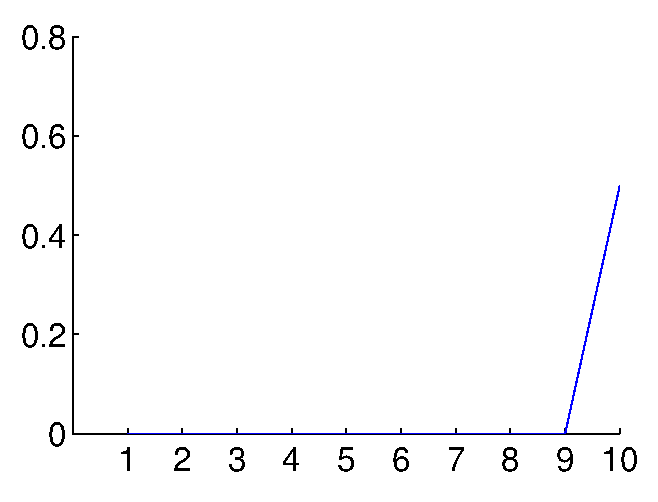
\includegraphics[width=0.20\textwidth]{figures/experiments/comparison/fdeawithoutclusterdtlz1_10.eps}
	}	
	\hspace{0em}	
	\subfigure[\textit{F}-DEA$^{\#}$]
	{
		\label{fig:dtlz110fdeahashfigure}
		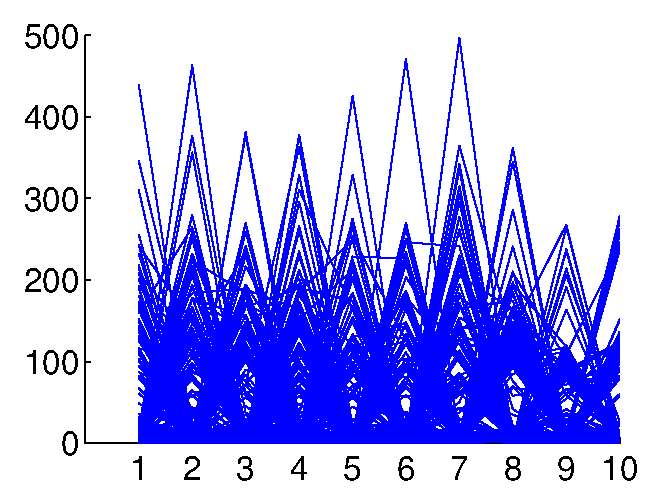
\includegraphics[width=0.20\textwidth]{figures/experiments/comparison/fdeaparetodtlz1_10.eps}
	}	
	\hspace{0em}
	\subfigure[Basic \textit{F}-DEA]
	{
		\label{fig:dtlz110fdeafigure}
		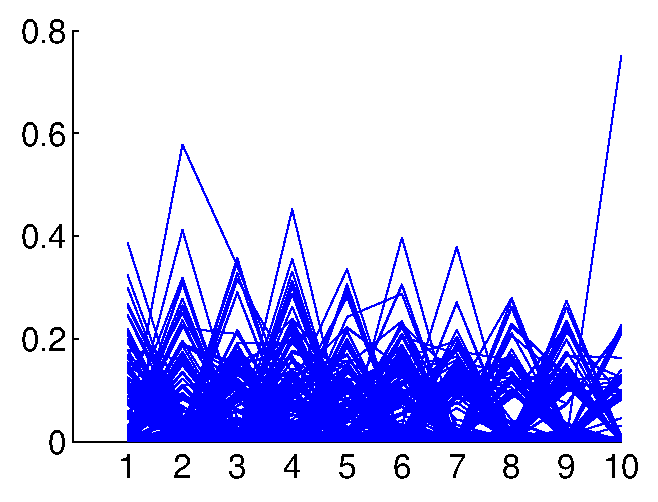
\includegraphics[width=0.20\textwidth]{figures/experiments/comparison/fdeagausdtlz1_10.eps}
	}
\caption{Parallel coordinate plots of variants of $F$-DEA on $10-$ objective DTLZ1 problem. }
\label{fig:dtlz110figure}
\end{figure}
\begin{table}[]
\centering
\caption{Comparison among three different versions  of the proposed algorithm,  basic version ($F$-DEA), $F$-DEA without clustering ($F$-DEA$^{*}$), and $F$-DEA with Pareto dominance ($F$-DEA$^{\#}$), on DTLZ problems based on IGD and 
HV value.}
\label{table:dtlzigdvariant}
%\setlength{\tabcolsep}{2pt}
\renewcommand{\arraystretch}{1.1}
\begin{adjustbox}{width=0.50\textwidth,center}
\begin{tabular}{ccccc}
\thickhline
\multicolumn{5}{c}{IGD}\\\thickhline 
%\multicolumn{5}{c}{HV}\\\thickhline 
Prob. & Obj. & $F$-DEA$^{*}$ & $F$-DEA$^{\#}$ & $F$-DEA                      \\\thickhline
DTLZ1 & 7    & 0.0296$\pm$0.0152(2)  & 9.0918$\pm$1.5703(3)  & \textbf{0.0063$\pm$0.0001(1)} \\
      & 10   & 0.0302$\pm$0.0155(2)  & 7.6205$\pm$1.1507(3)  & \textbf{0.0083$\pm$0.0002(1)} \\
      & 15   & 0.0269$\pm$0.0159(2)  & 5.8475$\pm$1.1274(3)  & \textbf{0.0094$\pm$0.0002(1)} \\\thickhline
%DTLZ2 & 7    & 0.0858$\pm$0.0000(2)  & 0.1602$\pm$0.0014(3)  & \textbf{0.0175$\pm$0.0005(1)} \\
%      & 10   & 0.0877$\pm$0.0000(2)  & 0.1357$\pm$0.0108(3)  & \textbf{0.0223$\pm$0.0006(1)} \\
%      & 15   & 0.0855$\pm$0.0000(2)  & 0.1015$\pm$0.0074(3)  & \textbf{0.0250$\pm$0.0009(1)} \\\thickhline
DTLZ3 & 7    & 0.0861$\pm$0.0001(2)  & 83.6979$\pm$7.0178(3) & \textbf{0.0528$\pm$0.0418(1)} \\
      & 10   & 0.0905$\pm$0.0120(2)  & 70.5014$\pm$6.9913(3) & \textbf{0.0396$\pm$0.0246(1)} \\
      & 15   & 0.0856$\pm$0.0001(2)  & 56.6080$\pm$6.5905(3) & \textbf{0.0510$\pm$0.0317(1)} \\\thickhline
%DTLZ4 & 7    & 0.0858$\pm$0.0000(2)  & 0.1517$\pm$0.0034(3)  & \textbf{0.0178$\pm$0.0003(1)} \\
%      & 10   & 0.0877$\pm$0.0000(2)  & 0.1056$\pm$0.0069(3)  & \textbf{0.0225$\pm$0.0005(1)} \\
%      & 15   & 0.0855$\pm$0.0000(3)  & 0.0729$\pm$0.0066(2)  & \textbf{0.0224$\pm$0.0005(1)}\\\thickhline 
      \multicolumn{5}{c}{HV}\\\thickhline    
      DTLZ1 & 7    & 0.1410$\pm$0.0723(2)  & 0.0000$\pm$0.0000(3) & \textbf{1.9272$\pm$0.0026(1)} \\
      & 10   & 0.1877$\pm$0.0963(2)  & 0.0000$\pm$0.0000(3) & \textbf{2.5829$\pm$0.0024(1)} \\
      & 15   & 0.2839$\pm$0.1682(2)  & 0.0000$\pm$0.0000(3) & \textbf{4.1680$\pm$0.0021(1)} \\\thickhline
%DTLZ2 & 7    & 0.1771$\pm$0.0000(2)  & 0.0000$\pm$0.0000(3) & \textbf{1.7469$\pm$0.0045(1)} \\
%      & 10   & 0.2357$\pm$0.0000(2)  & 0.0004$\pm$0.0019(3) & \textbf{2.4854$\pm$0.0059(1)} \\
%      & 15   & 0.3797$\pm$0.0000(2)  & 0.0000$\pm$0.0000(3) & \textbf{4.1171$\pm$0.0083(1)} \\\thickhline
DTLZ3 & 7    & 0.1684$\pm$0.0053(2)  & 0.0000$\pm$0.0000(3) & \textbf{0.8720$\pm$0.7061(1)} \\
      & 10   & 0.2156$\pm$0.0511(2)  & 0.0000$\pm$0.0000(3) & \textbf{1.7546$\pm$0.9708(1)} \\
      & 15   & 0.3683$\pm$0.0096(2)  & 0.0000$\pm$0.0000(3) & \textbf{2.2773$\pm$1.8582(1)} \\\thickhline
%DTLZ4 & 7    & 0.1771$\pm$0.0000(2)  & 0.0000$\pm$0.0000(3) & \textbf{1.7540$\pm$0.0025(1)} \\
%      & 10   & 0.2357$\pm$0.0000(2)  & 0.0001$\pm$0.0004(3) & \textbf{2.4951$\pm$0.0023(1)} \\
%      & 15   & 0.3797$\pm$0.0000(2)  & 0.0491$\pm$0.0596(3) & \textbf{4.1402$\pm$0.0019(1)}\\\thickhline
\end{tabular}
\end{adjustbox}
\end{table}
%\input{dtlzhvvariant}
%\input{wfghvvariant}



\subsection{Parameter Sensitivity}
\label{subsec:parametersensitvity}

In the absence of supplied reference points, $F$-DEA employs the Das and Dennis~\citep{das1998normal} procedure for generating such points. This procedure requires a parameter $\lambda$, the number of division in an objective. 
It is worth mentioning that  $\lambda$ is necessary if any evolutionary algorithm (see, for example, ~\citep{deb2014evolutionary}) employs this procedure. 
The aim of this section is to show why we select $p$ (=$N$, the population size) preferred points from a large number of generated points.

%Having parameters is a less desired property for any algorithm because they require tuning for different scenarios, which is inconvenient for a decision maker. However,  $\lambda$ and $p$ used in $F$-DEA give the necessary flexibility to the decision maker's desires. One can ignore $\lambda$ if the supplied reference points to the preferred directions are available. If the decision maker does not want to (or cannot) supply   reference points due to lack of domain knowledge, $\lambda$ works in such a case. 
%The other parameter $p$  gives  freedom to control over convergence and diversity. 
Trivially, an evolutionary algorithm maintains diversity and convergence by its own way, where the decision maker has no control. 
In $F$-DEA, the decision maker can control them using $p$. Furthermore, $\lambda$ and $\ p$ together remove the constraint to population size for any number of objectives unlike NSGAIII~\citep{deb2014evolutionary,thetadominance7080938} in which the population size is bounded by $\lambda$ and not flexible for an arbitrary number of objectives.

Fig.~\ref{fig:parametersensitivty} shows impact of $\lambda$ and $p$ on the GD, IGD and HV performances of DTLZ2 problem with $10$-objective. The experiments were conducted with the usual parameter settings but varying $\lambda$ and $p$. For convenience, $p$ was changed in such a way that the expected number of solutions in each cluster, $\chi$, becomes $2, 3, \cdots,10$.

We can see as $\lambda$ increases so does overall HV (Fig.~\ref{fig:dtlz210hvparameter}) and reduces GD (Fig.~\ref{fig:dtlz210gdparameter}) and IGD (Fig.~\ref{fig:dtlz210igdparameter}) up to a certain level. Increasing $\lambda$ increases the number of generated reference points exponentially. A small number of reference points do not cover the entire objective space. Generating a large number of reference points maintains better cluster uniformity which in turn improves overall performance. But if we continue increasing reference points then after a certain $\lambda$, the clusters' representative points will be nearly same as before and performance will be clipped. It is also expensive to generate a huge number of reference points. Hence, a reasonable number of  reference points should be used. By inspecting the performance on DTLZ2, it is clear that  after $\lambda=9$ the performance doesn't improve increasing $\lambda$~(Fig.~\ref{fig:parametersensitivty}). It is to be noted that HV for $\lambda=3$ is greater than the HV value for $\lambda=4$ and this behavior is problem dependent. Therefore it is sufficient to use $\lambda = 9$ for $10$-objective problem. 


As $p$ decreases, the number of clusters decreases and the expected number of solutions, $\chi$, in a cluster increases for a fixed-size combined population, $\left|C_t\right| = 2N$ (e.g. for $p = N$, $\chi=2N/N=2$ and for $p = \frac{N}{2}$, $\chi = 2N/\frac{N}{2} = 4$).
The fuzzy dominance relation within a cluster promotes faster convergence. By decreasing $p$, the solutions achieve faster convergence while losing some diversity. A closer inspection of Fig.~\ref{fig:dtlz210gdparameter} reveals  that as $p$ decreases (i.e., increasing $\chi$), the overall GD value decreases i.e., convergence increases. The overall performance of HV decreases~(Fig.~\ref{fig:dtlz210hvparameter}) and IGD value increases~(Fig.~\ref{fig:dtlz210igdparameter}), which indicates reduction in diversity. Therefore $p=N$ or $\chi=2$ is  preferable as it works as the best compromise between convergence and diversity.
We might require more converged optimal solutions compromising some diversity in some real-world applications. It is possible to achieve this goal by decreasing $p$. An opposite scenario i.e., obtaining more diverse solutions can also be achieved by increasing $p$.

%By increasing $p$, the preferable cluster size, we get more diverse solutions and by decreasing $p$ value we get faster convergence. Combining convergence and diversity sensitivity together in adaptive manner will also work. For example giving convergence a boost at the beginning of generation and diversity later (although in this case domain knowledge will be required for generating well distributed random solutions at the start) by starting with smaller $p$ and increment $p$ later. We left this as a further studies for future work.

%\input{parameterplot}
%\input{parameterSensitivity}
\input{latexinput/parameterSensitivityDtlz}


\section{Conclusion and Future Work}
\label{sec:conclusion}

Evolutionary algorithms can provide several candidate solutions in a single run, which make them popular to solve many practical problems including MaOPs. However, the loss of selection pressure is a challenging issue for such algorithms while solving MaOPs. 
In this paper, we have incorporated fuzzy-dominance and reference points in the environmental selection mechanism of the proposed  
$F$-DEA with an aim of improving selection pressure. The introduction of reference point in conjunction of fuzzy-dominance not only helps in maintaining diversity of the evolved solutions but also convergence.

$F$-DEA has been extensively evaluated and compared using eight WFG and three DTLZ problems having 2- to 25-objectives. %It has also been evaluated and compared to three instances of Rectangle problem.
The simulation results reveal that $F$-DEA in general performs better than other algorithms on complex problems with an increasing number of objectives. 
It has also been found that $F$-DEA can balance between the conflicting goal of convergence and diversity well in comparison with other algorithms, especially for complex problems.

In its current implementation, the reference point generation procedure~\citep{das1998normal} used in $F$-DEA has one user-specified parameter, which was set after some preliminary experiments. One of the future avenues would be to make it adaptive. It would be interesting in the future to analyze $F$-DEA further and identify its strength and weakness. It would also be interesting to apply $F$-DEA to real-world problems. %and to extend $F$-DEA to solve constrained many-objective problems.

\section*{References}

\bibliography{fdeabibliography}

\end{document}